\documentclass[11pt, a5paper, twoside]{book}

\usepackage{float} % incluir imagens
\usepackage[export]{adjustbox} % centralizar
\usepackage{subcaption} % legendas
\usepackage{graphicx}
\graphicspath{ {pic/} }

\usepackage{geometry}
\geometry{a5paper, left=2.7cm, right=2cm, bottom=2cm, top=2.5cm}

\usepackage{setspace}
\singlespacing

\usepackage{indentfirst}
\usepackage[skip=0pt, indent=1.25cm]{parskip}

\usepackage{ragged2e}
\justifying{}

\usepackage[portuguese]{babel}
\usepackage{hyphsubst}

\usepackage{emptypage}

\usepackage{fontspec}
\usepackage{hyphenat}
\hyphenation{
    pre-pa-ra-va=me 
    trou-xe 
    ar-ras-ta-va=se 
    res-trin-giu=se
    a-co-mo-dou=se
    nun-ca
    mos-tran-do=se
}

\newenvironment{dedication}{
    \clearpage
    \thispagestyle{empty}
    \vspace*{\stretch{3}}
    \small
    \itshape
    \raggedleft
}{\par\vspace*{\stretch{1}}\cleardoublepage\normalfont\justifying} % taken from https://tex.stackexchange.com/questions/476646/how-put-title-in-a-dedication

\title{História da Família, Parte II}
\author{Teresa Cristina}
\date{2025}

\renewcommand{\thechapter}{\Roman{chapter}}

\addto\captionsportuguese{
    \renewcommand{\contentsname}{Sumário}
}

\begin{document}

\begin{titlepage}
\maketitle 
\end{titlepage}

\begin{dedication}
Aos meus filhos, para que, tal como ensinou Terêncio, nada que seja humano, seja-lhes estranho. 

Aos que cobrarem maior fidelidade aos fatos, saibam que o que aqui vai contado, vai tal e qual a emoção esculpiu na alma e a memória arquivou sem contestar. 
Pois nunca sabemos com exatidão o que de fato acontece. 
O que fica é o que nos parece e como nos parece no momento do acontecido. 
\end{dedication}

\tableofcontents

\chapter{}
Sou do tempo bom em que os adultos se livravam das crianças sem culpa, mandando: ``Vão brincar lá fora!''.
E ``lá fora'' era o quintal, o maravilhoso país da infância.
Sobretudo quando se vivia numa cidade do interior. 
Era o espaço de descobrir e pensar o mundo. 
Observar as formigas na sua labuta incessante, as lagartixas subindo pelo velho muro meio rachado, as borboletas iridescentes, o rastro prateado e gosmento desenhado pelos vagarosos caracóis.   
Contemplar a incessante migração das nuvens que o vento ora esfiapava, ora ia juntando em formas caprichosas de bichos, árvores, gigantes, castelos, anjos e às vezes mapas, como aqueles pendurados nas paredes da sala de aula. 
Sentir o cheiro da roupa lavada e embebida de sol, pendurada no varal; da fumaça desprendendo-se da lenha queimada no fogão; da terra molhada, da moita de arruda, das rosas, do jasmim, do manacá; do bafio úmido de sepulcro que emanava da escura caverna do porão. 
Deitada de costas nas pedras quentes da calçada, abandonava-me ao sol. O calor invadia aos poucos meu corpo, amolecendo braços e pernas e eu os imaginava penetrando terra adentro, como raízes. 
Imóvel, escutava o zunido das abelhas nas flores, os recados insistentes do ``fogo apagou'' e do bem-te-vi vindos lá das bandas do cemitério, o canto dos sabiás e a algazarra dos pardais e andorinhas sobrevoando a velha paineira do almoxarifado da prefeitura bem ali, do outro lado da rua. 
Na marcenaria, alguns quarteirões acima, o som plangente da serra cortando madeira dividia com o sino da torre da Matriz a tarefa de marcar regularmente a passagem das horas. 
Vez ou outra, roncando em agonia a cada mudança de marcha, os velhos ônibus a querosene passavam sacolejando nos paralelepípedos, rua acima; os carros ainda eram raros. 
E, do outro lado do muro, do barracão da fábrica do meu pai, chegava o som oceânico, abafado e constante das máquinas torcendo os fios de algodão para transformá-los nos novelos de barbante que garantiam o sustento da nossa família e a minha doce vadiagem de criança.

As cores, formas e textura das flores e folhagens me fascinavam. 
Recobriam meus desenhos infantis e emolduravam em cercaduras delirantes as páginas dos meus cadernos de escola.

Na opinião da minha mãe, as flores do nosso quintal deviam obedecer à moda, como tudo o mais. 
Lembro-me da fase dos crisântemos, dálias e crisandálias repolhudas, logo repudiadas em favor das rosas que, por sua vez, acabaram arrancadas para dar lugar às palmas de Santa Rita e às gérberas. 
Essas mudanças eram quase sempre decididas por volta do Dia de Finados, quando as parentes da Capital chegavam sobraçando as novidades compradas nas floriculturas do Arouche. 
Houve uma vez em que a matriarca das hostes paulistanas, Tia Angelina, desceu do trem exibindo buquês de soberbos e inacreditáveis gladíolos azuis. Foi o quanto bastou para que as nossas pobres palmas de Santa Rita caíssem em desgraça. 
``Coisa mais calú!'', decretou minha mãe. 
Era sua expressão favorita para o que lhe parecia vulgar ou caipira. O projeto do novo jardim teve, porém, que ser adiado. 
De tanto mexer na terra, nas sucessivas reformas dos nossos canteiros, mamãe arrumou uma infecção persistente nos dedos que acabou por lhe fazer caírem as unhas. 
Até um médico especialista em São Paulo precisou ser consultado, já que o nosso habitual curandeiro, o Joãozinho da Farmácia, amigo de longa data do papai, não conseguiu resolver a tal eczema.

De qualquer modo, outros e mais amplos planos de mudança começavam a agitar minha família, pois mamãe começara a achar ``calús'' não só as flores, como todo o quintal, a casa antiga de ``parede a meia'' e banheiro fora, os móveis escuros, ``art-déco''. 
Papai prosperava nos negócios e mamãe já podia sonhar mais alto: uma casa moderna, com mais cômodos, armários embutidos, num bairro novo e mais nobre. 
Prenunciando a nova fase, nossa antiga sala de jantar desapareceu para dar lugar a uma mobília nova e aromática, de jacarandá torneado, em que se destacava uma vistosa cristaleira apropriadamente recheada com copos de cristal recém-adquiridos e que tilintavam perigosamente a cada passo nosso sobre o velho assoalho. 
Nossas caminhas \textit{Patente} foram substituídas por outras, artisticamente torneadas também e os velhos colchões de crina foram para o lixo. 
Passamos a dormir em modernos colchões de mola. Um tapeceiro alemão veio tirar as medidas para fabricar sofá, poltrona e cortinas para a sala de estar. 
Coroando todo esse luxo, um dia desembarcou em nosso portão a peça central da nova decoração: um piano de nogueira, novo em folha, que se converteria num dos grandes instrumentos de tortura da minha juventude. 
Porque então, junto com o quintal e a velha casa, ficava para trás também a minha infância. 
Eu me tornara uma adolescente e, em breve, nós mudaríamos para a casa da Av. D. Pedro II, n.º 1273, defronte ao Clube de Campo do Araraquarense. Corria o ano de 1958.

\begin{figure}[H]
\centering
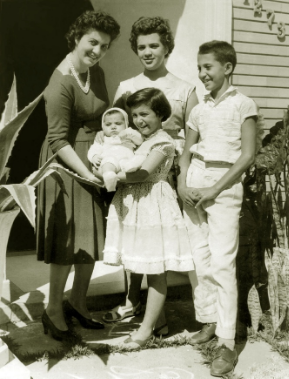
\includegraphics[width=0.5\linewidth]{1/maria-joão.png}
\caption{A família na porta da casa nova. No colo da
Maria Lúcia, o recém-chegado João.}
\end{figure}
\chapter{}
Para o bem e para o mal, minha infância transcorreu numa pequena galáxia de clãs interligados, de origem imigrante e pobre, dos quais os mais importantes eram os Filpi, os Credidio e os Ópice, todos com raízes na Itália. 
Dezenas de olhos e bocas para censurar e orientar e montes de braços para acarinhar e acolher, e uma intensa experiência humana para vivenciar, recolher, degustar e aprender. 

Nossa antiga sala de jantar exibia uma mesa particularmente desgraciosa, quadradona e pesada, mas que, para mim, tinha um encanto especial: embutia um pequeno armário no seu único e largo pé central, onde eram guardados os jornais velhos. 
Um dia descobri que eu cabia direitinho naquele esconderijo e ali, insuspeitada, colhi minhas primeiras e fortes impressões do mundo adulto.  
Era à volta daquela mesa que as visitas se reuniam para o café. 
Era divertido acompanhar, debaixo dela, o movimento das pernas inchadas e nodosas de varizes das tias-avós, na excitação de comentar os acontecimentos da cidade e a vida alheia. 
Quando mamãe e suas irmãs aparteavam a discussão, vez ou outra, contrapondo argumentos mais modernos, arejados por visões do pós-guerra de liberação feminina, difundidas pelo cinema norte-americano quase sempre, as vozes se alteravam, os pés se agitavam e, na ânsia de vencer a contenda, de algum ponto da mesa vinha a cartada definitiva, o disse-me-disse mais recente e irretorquível, quase sempre sussurrado, inalcançável à minha parca compreensão de criança, mas emoldurado pela aura sagrada e misteriosa do interdito\dots 
Um \textit{``oooohhhh!''} seguido de horrorizado silêncio parecia encerrar a conversa. 
Que logo, porém, renascia animada, como fogo sob as cinzas, sempre sublinhada embaixo da mesa pelo entusiasmado balé de pernas e pés. 
Lembro, com nitidez, de uma tarde em que, andando com minha mãe pela rua, ouvi-a chamar a atenção de uma amiga para uma célebre senhora, personagem recorrente nas reuniões à volta da tal mesa, pelo que me lembro, pelas audaciosas e repetidas incursões fora da sagrada cidadela do casamento. 
Olhei na direção indicada e vi uma mulher vestida de preto, grave e majestosa, na penumbra do banco traseiro de um carro escuro e grande.
Divisei-lhe as feições, ainda bonitas na maturidade. 
Séria, ela devolveu o meu olhar fascinado. E o que senti, juro, foi pura admiração.

Dos clãs principais, o da minha mãe era o mais pobre. 
Incluía as irmãs da minha avó Didi, seus maridos e filhos. 
Meu avô João já não tinha mais parentes próximos. 
Dele só conheci um primo engraçado, que vez ou outra aparecia e de novo sumia, como um cometa.  
Embora todas fossem casadas, as Credidio, mulheres invariavelmente fortes e batalhadoras, sobrepunham-se aos machos em autoridade. 
Dessa gente me vieram os impulsos de amar a vida, de superar os revezes sem esmorecer, de correr atrás dos sonhos, mas também a preocupação com as aparências alimentada pelo receio permanente de incorrer em vulgaridade e mau-gosto. 
Alimentavam ambições sociais e acreditavam piamente em cultivar as boas relações para vencer as desvantagens da origem humilde.  
No riso e no pranto, eram pau para toda obra. Com a mesma disposição para encarar bailes e velórios, casamentos, batizados e procissões, envolviam-se em tudo com igual disposição de fazer todo o necessário para que tudo saísse perfeito. 
Davam-se a todas essas empreitadas com sincera devoção e autêntico espírito de caridade e solidariedade. Mas, não dispensavam os holofotes e tinham a deliciosa ingenuidade de nem tentar disfarçar o prazer que sentiam com a repercussão favorável.

O clã do meu pai, os Filpi, embora menos pobre na sua origem, na Itália, já conhecia há muito a inconstância dos fados. 
Lá, na pequena Novi Velia, o patriarca Ângelo viu seus bens esvaírem-se no torvelinho das brigas políticas. 
Aqui, seu filho e meu avô Reginaldo, fazendeiro abastado a quem o café proporcionara razoável fortuna, casa confortável na cidade e educação de qualidade para a prole, perdeu quase tudo na crise de 1929 e teve que levar a família de volta ao recomeço duríssimo na Pedra Branca, única fazenda que lhe restou das quatro ou cinco que chegou a possuir. 
Por conta desses reveses, com certeza, dessa gente me veio um realismo prudente, alicerçado na crença de que estamos cá na terra a serviço e não a passeio, na desconfiança de que todo ídolo oculta pés de barro e de que tudo que reluz quase nunca é ouro, além do mau hábito de trabalhar até o limite das forças. 

O reino das mulheres Filpi era o lar. 
Exímias cozinheiras, incansáveis no lavar, passar, esfregar, bordar e tecer, foram condenadas à vida espartana pelo atraso da minha avó Teresa, uma mente forjada pelo rígido código dos antigos costumes mineiros. 
Mulher era para servir ao homem, pai, irmão ou marido e não para bater pernas na rua e perder-se como as moças pintadas, ataviadas e oferecidas que se viam por aí, querendo diploma, frequentando bailes, usando saias curtas, dirigindo e até fumando! Quando minha mãe, professora formada, frequentadora contumaz dos bailes do clube, exibindo impecáveis unhas esmaltadas e envergando trajes e penteado da moda ingressou na família, não fosse o apoio imediato do galante sogro Reginaldo, certamente seria rechaçada como péssimo exemplo. 
E pelo resto da vida, mesmo após a morte da Vó Teresa, a relação da minha mãe com as cunhadas, foi contraditória: Lectícia era o farol que iluminava para elas os difíceis caminhos da inserção social e da modernidade. 
Mas mamãe, por muitos e muitos anos, padeceu da necessidade neurótica de provar que, apesar das unhas feitas e das roupas da moda, era páreo para elas no comando de um fogão, de um ferro de passar e no brilho das panelas. 
Daí por que preparar um almoço para as cunhadas era um feito precedido por dias de insuportável e cômica tensão, mas que valiam pelo gosto insuperável da vitória, quando o molho e a massa se apresentavam indiscutivelmente no ponto certo. 
Por outro lado, as tias, com meu ouvido treinado em escutar conversa de adultos, ouvia-as muitas vezes lamentar o destino do irmão, coitado, condenado a trabalhar para sustentar os luxos ``daquela gastadeira''.

Os Ópice eram oriundos do casamento de duas irmãs da minha avó materna com dois irmãos recém-chegados da Itália e que vieram estabelecer-se em Araraquara: um hábil alfaiate, chamado Bruno e um não menos hábil carpinteiro chamado José. 
Ao que se conta, ambos exibiam como característica principal um certo refinamento de gostos, incomum entre os pobres imigrantes italianos da região e que provavelmente lhes pareceu suficiente para justificar uma postura algo arrogante e prepotente que sempre os distinguiu, tanto quanto os rompantes de temperamento. 
Afora isso, eram muito trabalhadores e competentes. Todos esses traços são ainda bem visíveis na sua descendência. 
O ramo do Tio Bruno, quase todo, enraizou-se em definitivo na cidade e o do Tio José, algum tempo após a morte precoce deste, acabou migrando para a Capital. 
Os filhos do Tio Bruno, que continuaram a viver sob o jugo do pai, jamais amadureceram totalmente e ficaram na minha memória como uma família de gente boa, meio infantilizada e divertida. 
Os órfãos do Tio José, libertos do autoritarismo paterno, com muito mérito e muito trabalho, fizeram carreira e sólida fortuna na capital. 
E foi assim que se transformaram, para toda a gente da minha mãe, na referência suprema do sucesso, do ``savoir faire'', o exemplo a ser seguido, fonte de jurisprudência a ser consultada em qualquer circunstância e para qualquer assunto. 
Eram respeitosamente designados como ``os de São Paulo'' e sempre que vinham em visita aos parentes da província provocavam um alvoroço que, à medida que nós, os mais novos, crescíamos, acabou virando motivo de piadas sempre recebidas como sacrilégio por vovó, mamãe e suas irmãs. 
Já meu pai que, como bom Filpi, nunca foi afeito a idolatrias de qualquer espécie, fechava o tempo e não foram poucas as vezes em que os pobres Ópice acabaram pagando pela admiração incompreensivelmente servil, no entender do marido, que minha mãe devotava às ideias e realizações dos primos.
\chapter{}
Em meados do século XX, o castigo físico para a meninada não só continuava em pleno vigor, como em doses razoáveis era considerado instrumento eficiente na construção do caráter infantil. 
Já não se usava a palmatória nas escolas, mas ``a régua cantava'' regularmente nas salas de aula sem que alunos ou pais pensassem em recorrer à justiça por causa disso. 
Era até de bom-tom, como testemunho de confiança e parceria, que estes últimos, ao entregar seus filhos aos mestres, delegassem a eles a prerrogativa de puxar-lhes as orelhas sempre que necessário.

Herança do meu avô Reginaldo, na minha casa havia um \textit{rabo-de-tatu}, uma espécie de chicote feito com pouco mais de três palmos de couro de sola, grosso, arrematado por um cabo trançado em torno de uma argola de metal pela qual ficava pendurado atrás da porta da cozinha. 
Originalmente, tal instrumento era usado para espicaçar a montaria. Como meu avô era exímio cavaleiro e vivia de chicote em punho, deve ter sido só uma questão de oportunidade para que o artefato se convertesse em recurso pedagógico. 
Por sorte, na maioria das vezes, o rabo de tatu da minha casa servia mais à intimidação do que ao uso propriamente dito. 
As surras ``para valer'' eram ministradas sempre pelo meu pai que, explosivo como era, preferia usar suas temíveis manoplas ao invés de perder tempo indo atrás do tal relho. 
Minha mãe é que às vezes o usava para potencializar a escassa força dos seus punhos femininos. Mas, na maior parte do tempo ela recorria apenas aos beliscões, aos tapas e às ameaças:

{\itshape “ -- Deixa estar! Vou contar tudo ao seu pai quando ele chegar e aí eu quero ver!”}

Essa história de apanhar me parecia revoltante pelo que atentava contra a dignidade das pessoas. 
Sentia-o mesmo quando muito menina para sabê-lo. 
Minha mãe apenas me irritava quando me batia, mas com meu pai era diferente.  
Principalmente porque eu tinha uma forma peculiar de reagir ao medo e que redundava numa humilhação ainda maior: eu me urinava todinha, só de pressentir a iminência do seu ataque de cólera. 
Bastava que ele entrasse porta adentro me chamando e escandindo as sílabas do meu nome, anúncio inequívoco das bofetadas que viriam. 
As pernas amoleciam e eu me agachava, passiva, em meio à poça que se alastrava em torno de mim. Com o tempo, percebi que o meu terror parecia aplacar-lhe a ira. 
Eu acabava apanhando menos que meu pobre irmão que, rebelde, usava toda a agilidade das suas magras perninhas para fugir, certo de que papai, pesado e lento, jamais conseguiria alcançá-lo. 
Mas a estratégia se revelava pior. Mais enfurecido, quando lhe punha as mãos, meu pai parecia perder a noção da absurda desproporção entre o seu tamanho e o da frágil criança. 
Mais de uma vez circunstantes assustados intervieram com medo de que ele arrebentasse o menino. 

Apanhamos com alguma constância, meu irmão e eu até a adolescência. 
Não porque evidenciássemos uma inclinação acentuada para a delinqüência. 
Ao contrário. 
Éramos bons alunos e nosso repertório de travessuras nunca excedeu o limite do esperado numa época em que as crianças “eram para ser vistas, mas não ouvidas”. 
Reginaldo era um garoto vivo e muito esperto. 
Foi sempre festejado por essas características e, até onde me lembro, meus pais pareciam orgulhosos em ressaltá-las sempre que se referiam ao filho. 
Apanhar por causa disso devia causar uma grande confusão na cabeça dele. Já eu, que Vó Didi chamava de “minha pata-choca”, precisava de uma razão muito forte para sair da minha habitual bonomia. 
Também não conseguia entender o porquê das surras.

\begin{figure}[H]
\centering
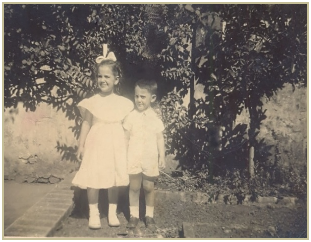
\includegraphics[width = 0.9\linewidth]{3/Reginaldo.png}
\caption{Reginaldo e eu por volta de 1950.}
\end{figure}

Uma das primeiras grandes sovas que levei, lembro, foi no Jardim da Infância porque havia, na escola, a atribuição semanal de uma “Medalha de Disciplina” aos que demonstravam melhor comportamento ao longo da semana e num sábado, excepcionalmente, eu não a trouxe para casa. 
Minha professora me deixara tomando conta dos meus vinte e poucos coleguinhas para dar uma escapadela, sabe-se lá para onde e um deles me pediu que deixasse a turma escrever na lousa. 
Com o discernimento a mim conferido pelos meus seis anos, achei que aquela seria uma boa forma de mantê-los ocupados. 
Não foi. 
Quando a professora retornou, havia giz para todo lado e um realizado e barulhento grupo de pirralhos tinha transformado não só a lousa como todas as paredes da sala numa exposição surrealista, sem que eu, impotente, conseguisse contê-los. 
Meu pai nem quis ouvir a história. 
Ainda hoje acho que a professora, D. Lídia, é que devia ter apanhado em meu lugar. 
 
Na família da minha mãe esse tratamento não existia. 
A menos que se levasse em consideração os beliscões e alfinetadas que marcavam os momentos relevantes dos sermões da Vó Didi às filhas adolescentes, enquanto lhes experimentava as costuras. 
Mamãe achava que ela reservava esse momento de propósito para os corretivos. O
Vô João, ao contrário, não só jamais se agastava como se apressava em protegê-las das tempestades maternas. 

Já na família do meu pai, o emprego da força física para dirimir questões de qualquer natureza era um valor muito apreciado. 
Vó Teresa, contava minha mãe, jactava-se de que seus filhos eram homens de resolver qualquer parada “com um soco só”. 

Um fato lembrado com divertida alacridade pelos irmãos Filpi, e exemplo amplamente divulgado do que acabo de relatar, dizia respeito a uma façanha perpetrada por um deles, o Tio Bepe, um rotundo peso-pesado de cento e trinta quilos, quando desconfiou que Tia Antonieta e Tia Glória, suas irmãs e noivas de dois irmãos, proprietários de uma vidraçaria, estavam sendo iludidas. 
Como a data do casamento ia sendo prorrogada ``ad infinitum'' pela família dos rapazes, ele decidiu tomar satisfação com os infelizes vidraceiros que, pálidos de terror, mal conseguiram entender o motivo da intempestiva visita, comunicado aos berros por cima do crepitar dos vidros pulverizados a murros por aquele búfalo ensandecido. 
Nem é preciso acrescentar que, com o estabelecimento, veio abaixo também o sonho das pobres moças de um dia se casarem. 

O castigo físico como recurso educativo era praticado com naturalidade e frequência entre os Filpi. 
Ouvi minhas tias aludirem, mais de uma vez, a uma bizarra norma pela qual, em crianças, quando um cometia uma falta passível de castigo, todos apanhavam para que um não caçoasse do outro. 
E papai lembrava com muito ressentimento uma passagem em que, muito pequeno ainda, distraíra-se observando formigas, deitado de bruços, espichado ao sol, ao invés de varrer o terreiro de café como lhe tinha sido ordenado.  
Sem dizer água vai, o avô Reginaldo, lá da varanda, fez estalar o comprido látego de conduzir charrete e desenhou-lhe um vergão em brasas ao comprido das costas. 
Revoltou-o demais o gesto tão violento quanto traiçoeiro. 
O que não o impediu de, ao crescer, acrescentar sua própria contribuição ao longo prontuário de brutalidades dos Filpi. 
Vovó Teresa nada ficava a dever ao marido no que diz respeito ao emprego da força como recurso disciplinar. 
Ao contrário, dado que Vovô se ausentava com freqüência, na maioria das vezes era a ela que cabia exemplar a numerosa prole. 
Mamãe contava ter presenciado uma cena em que tia Antonieta, a que mais ansiava por uma história de vida diferente daquela que levava em regime de semi-clausura, foi pedir à mãe permissão para continuar os estudos. 
Em resposta, recebeu tamanho safanão que perdeu o fôlego e a fala por longos e angustiantes segundos. 
E ela já era uma mocinha, a coitada.

Não é de admirar que os irmãos Filpi, incluídas aí as mulheres, uma vez adultos, fossem estimados e respeitados pelas numerosas qualidades de diligência, honestidade, generosidade, disponibilidade para com as necessidades do outro, mas igualmente temidos pela fúria demolidora que lhes podia brotar das entranhas quando enraivecidos.  
Naquele tempo, porém, no que toca aos machos da família, esta característica não chegava a causar grande escândalo porque encontrava certo amparo na mentalidade que predominava, como ainda predomina em alguns rincões da nossa sociedade, de que só pelo uso da força bruta um homem se legitima como tal. 
E o público feminino, não se pode negar, só recentemente começou a limitar seu entusiasmo por esse gênero de exibição. 
Mais de uma vez surpreendi uma expressão de orgulho na fisionomia da minha mãe quando meu pai se impunha pela força dos seus músculos. 
E ele nem precisava disso. 
Tinha estatura moral mais do que suficiente para conquistar naturalmente a admiração e o respeito de quantos o conheceram, inclusive e principalmente nossos, dos seus filhos. 

De qualquer maneira, no caso do meu pai, pelo menos, tenho certeza de que a necessidade de afirmar sua autoridade por esse meio era uma das injunções que o atormentavam. 
Tanto que, após cada um desses surtos de raiva primitiva e indomável, ele parecia consumir-se em arrependimento e buscava por todos os modos uma maneira de compensar a vítima: um presente, um passeio, um agrado qualquer. 
Mas jamais conseguiu reagir de outra maneira a uma situação em que se sentisse desafiado.

\begin{figure}[H]
\centering
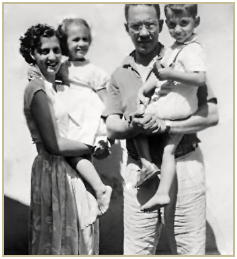
\includegraphics[width = 0.5\linewidth]{3/Familia.png}
\caption{Nossa família, no início dos anos 50.}
\end{figure}

Todos sabem que é contra o muro sólido do poder adulto que os jovens afiam seus dentes e garras. 
Seria preciso que meu pai fosse uma personalidade emocionalmente mais segura para suportar as investidas ditadas pela nossa imaturidade. 
Assombrava-o a possibilidade de cometer erros ou perder as rédeas na condução da família e na educação dos filhos. 
Porque, em nosso meio, esse seria o pior dos fracassos, o mais imperdoável, social ou pessoalmente falando. 
Ao contrário do que se ouve muitas vezes hoje, era opinião corrente que um filho desencaminhado expunha ao mundo a incompetência dos pais. 
Então, naquele tempo, mais que hoje em dia, à medida que a gente evoluía previsivelmente na direção da independência, os problemas em casa tendiam a aumentar na mesma proporção e o chamado “choque de gerações” sobrevinha com impacto terrível sobre as relações familiares. 
De alguma maneira, traumas a parte, esse conflito acabava por exercer uma força centrífuga de tal monta que raras vezes um jovem, depois de experimentá-la, desejava voltar para casa, a não ser depois que achasse um rumo na vida, ou seja, um diploma, um trabalho e até um casamento meio engatilhado. 
Essa podia não ser a forma mais adequada de pais promoverem a autonomia dos filhos, mas funcionava, sem sombra de dúvida. 
Os raros homens ou mulheres que permaneciam em casa, na dependência dos pais, além dos vinte e poucos anos, eram considerados indivíduos frustrados no seu desenvolvimento e olhados com um misto de piedade e estranheza.
As pessoas se perguntavam o que podia ter dado errado.  

Pode-se entender, neste contexto, a insegurança e as reações do meu pai, tendo sido ele próprio, além de tudo, um adolescente um tanto desajustado, sensível e difícil, que por pouco “não se perdeu por aí”, segundo contavam seus irmãos. 
Nele, como me acostumei a dizer, a rebeldia corcoveou até o fim sob a sela pesada da responsabilidade de homem de negócios e chefe de família. 
A repressão violenta exercida sobre nós, sobretudo os seus filhos mais velhos, hoje eu acredito, era também resultado de um esforço hercúleo para exorcizar sua própria inconformidade.

Aos catorze anos decidi que bastava. 
Quando num acesso de fúria meu pai levantou a mão para mim, encarei-o decidida a me defender, fosse como fosse. 
Acho que ele percebeu. Nunca mais repetiu o gesto. 
Paradoxalmente, entretanto, aquela manzorra pesada que tanto me apavorava quando se precipitava como aríete na minha direção, ficou na minha lembrança como a mesma que me comunicava tanta confiança e proteção quando se fechava, quente e firme, sobre minha pequena mão de criança.
\chapter{}
Entre cinco e seis anos, contraí uma infecção séria. Ao calçar-me os sapatos novos de ir à missa, minha mãe não conseguiu afivelá-los. 
Meus pés estavam estufados como bolos. 
Chamou papai e a fisionomia assustada de ambos me causou estranheza, já que eu não estava sentindo absolutamente nada. 
Mas logo comecei a gostar dos movimentos que se seguiram porque percebi que eu me tornava o centro de alguma coisa muito importante. 
Um médico foi chamado, o que de si já era incomum, pois todas as nossas indisposições eram ordinariamente atendidas pelo Joãozinho da Farmácia.
E quando o Dr. Newton, após examinar-me, ordenou repouso absoluto e dieta, a preocupação que se estampou na face dos meus pais me convenceu em definitivo de que naquele momento, nada mais importava na face da terra senão eu.  
Olhando em retrospectiva aquele momento e os meses que se seguiram àquela manhã, espanto-me com a descoberta de quanto senso dramático pode uma criança extrair de si e que insuspeitado talento ela pode manifestar em usá-lo. 
 
Embora a situação toda me fascinasse pelo muito de atenção que atraía sobre a minha pequena pessoa, a verdade é que o processo caminhou para uma quase tragédia. 
O tal médico, Dr. Newton, cometeu um equívoco no diagnóstico inicial e o que era uma simples infecção urinária evoluiu para uma nefrite. 
Dois meses depois, o crescente entra-e-sai de parentes e vizinhos no meu quarto atestava a gravidade progressiva do quadro. Exclamações como ``pobrezinha'', ``coitadinha'' e até ``santinha'', entreouvidas entre sussurros, tornaram mais doce o sorriso que eu abria para as pessoas. 
Vovó Didi ensinou-me uma cançoneta napolitana que falava em despedida e que com voz não menos doce eu cantava para as visitas, maravilhada em ver brotar-lhes lágrimas nos olhos. 
Eu continuava a não sentir nada, de modo que podia dedicar-me integralmente a desfrutar toda a intensidade das emoções que observava ao meu redor. 
Até que um dia, no final da tarde, um pequeno tumulto formou-se na sala em torno do meu pai que acabara de chegar da rua e entre gritos e choro sentido ameaçava matar o médico. 
Eu tinha sido desenganada. 
Nenhum outro médico aceitara levar adiante meu caso e todos haviam aconselhado vivamente a família a procurar com urgência um centro maior, com mais recursos.  Naquela mesma noite, numa tumultuada partida, embarcamos no trem noturno para São Paulo e de lá, de avião, para o Rio de Janeiro, onde nos aguardavam os dois irmãos médicos do papai, Tio Zico e Tio Ângelo. 
Quando finalmente meu pai pode me descer do colo ao chão no consultório do célebre nefrologista Prof. Laclette, um engraçado velhinho com jeito de Papai Noel, amontoei diante dele como um saco de batatas. 
Meus ossos haviam se transformado em gelatina durante o prolongado repouso. 

Ficamos por quase dois meses hospedados no Engenho Velho, na casa do Tio Ângelo. 
Era preciso primeiro vencer a infecção para que o foco de todo o mal que me afetara pudesse ser extirpado: eu tinha que retirar as amídalas. 

Meu anfitrião era casado com uma exótica e linda potiguar, tia Mariazinha, que, entre outras extravagâncias, era mãe-de-santo e dona de um terreiro de umbanda. 
Era, além disso, fantástica florista, chapeleira renomada e tinha, entre os animais domésticos, um grande e assustador cachorro preto, um mico endiabrado e uma jiboia obesa. 
Tudo isso somado tornava aquela casa meio mágica para mim, sensação que minha mãe estava longe de partilhar. 
As esquisitices da Tia Mariazinha pareciam demasiadas para ela. 
Principalmente quando, logo de manhã, a cunhada vinha lhe dar bom dia trazendo enrodilhada ao pescoço, como uma estola, a enorme cobra. Ou quando mamãe se punha a dedilhar o lindo piano alemão da sala e o mico, encarapitado no lustre, saltava-lhe diretamente nos ombros. 
Era louco por música, diziam.

\begin{figure}[H]
\centering
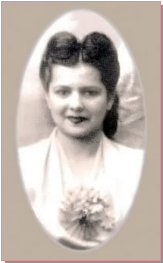
\includegraphics[width = 0.4\linewidth]{4/Tia Mariazinha.png}
\caption{A bela Tia Mariazinha.}
\end{figure}

Um acordo firmado entre marido e mulher vetava a realização de sessões de umbanda na casa. 
Para isso, Tio Ângelo havia concordado com a construção do terreiro, ou do Centro, como a Tia Mariazinha o chamava, num outro local. 
Entretanto, minha doença, ao que parece, forneceu à espevitada mãe-de-santo uma excelente oportunidade de provar a superioridade do poder dos orixás sobre a vã medicina dos civilizados. 
Logo ao chegar, eu tinha sido besuntada com óleos perfumados e metida num camisolão de flanela vermelha para desencorajar os maus espíritos. 
Em seguida, fui engalanada com voltas e voltas de guias de santo coloridas em torno do pescoço. 
Durante todo tempo em que lá estive até receber alta, foi vestida nessa flamejante indumentária que percorri consultórios e hospitais. 
Meus pais ficavam embaraçadíssimos, mas eu me achava linda. 

Como meu tio frequentemente passava noites de plantão na sua casa de saúde em Madureira, minha tia sentiu-se encorajada a ignorar o protocolo firmado com o marido e convocou seu pessoal para uma sessão noturna das importantes ali mesmo, no sagrado recinto do seu lar, já que eu, a paciente, não podia abandonar o repouso para ir ao terreiro. 
E foi desse modo que uma noite, no meio do sono, fui desperta para viver uma experiência inesquecível: no quarto semi-iluminado por velas, uma porção de gente vestida de branco entrava para dançar e cantar ao redor da minha cama, ao som do batuque ritmado dos atabaques. 
Mas o espetáculo maior era ela, minha tia: à frente de todos, numa roupa de alvura deslumbrante, enfeitada de colares, pulseiras e balangandãs, babados e mais babados de renda flutuando em imensa nuvem em torno do corpo, ela girava e sambava soberana, esplêndida Iemanjá! 
Pela primeira vez, vi os cabelos que ela arrumava em grosso rolo sobre a nuca, derramados em cascata negra e brilhante até abaixo da cintura. 
Sobre a cabeça, em equilíbrio milagrosamente inalterado pelos passos da dança, um copo de cristal com conchas e água do mar.
 Nunca mais me passou a vontade de um dia me vestir daquela maneira e dançar como a vi fazer naquela noite, deusa branca do candomblé. 
Dias depois, Tia Mariazinha achou necessário fazer uma nova sessão para reforçar os efeitos da primeira. 
Não vi o que aconteceu. 
A casa era um sobrado sólido, de grossas paredes, e eu já adormecera no andar de cima. 
Mas mamãe contou que meu tio chegou inesperadamente e o ritual foi abortado pela mais fulgurante explosão de ira que ela já tinha presenciado num Filpi. 
Caboclos, exus, babalaôs e babalorixás desceram desabalados rua abaixo. Não sobrou um para contar história. 

Ao fim de três semanas, já operada da garganta, comecei a melhorar e assim que me libertei do repouso, passei a freqüentar a oficina do quintal, onde a tia fazia inacreditáveis e delicadas camélias de veludo e cetim, rosas e violetas de organdi e seda e as arrumava em elegantes arranjos que as senhoras usavam à lapela dos ``tailleurs'', no decote, à cintura dos vestidos ``soirée'', ou ainda sobre a aba dos lindos chapéus que saíam daqueles dedos habilidosos e iam sendo arrumados em caixas sobre um tabuleiro enorme que depois ela punha à cabeça e, com seu displicente gingado de cabrocha, ia entregar nas casas das freguesas.

No aniversário da minha mãe, essa nordestina que jamais usou seu sofisticado bom gosto em favor de si mesma, orientou meu pai a comprar um corte de organza e renda francesas na ``Casa Canadá'', templo da moda carioca de então. 
Dentro da embalagem, sobre o negro transparente dos preciosos tecidos, colocou um ramo de rosas de organdi. 
Nunca vi outro igual. 
Foi o traje mais aristocrático que a minha mãe teve em toda sua vida. 

Uma semana depois, liberada já pelos médicos, preparava\hyp{}me para voltar para casa. Não sem antes conhecer o mar, o Corcovado, subir de bondinho o Pão de Açúcar e tomar sorvete na Confeitaria Colombo. 
Tinha viajado de trem e, suprema ventura, pela segunda vez ia tomar um avião. 
Na vinda tinha sido um Viscount e na volta seria um Constellation. 

Antes de partirmos, Tia Mariazinha exigiu que meu pai enchesse de moedas uma gamela de barro para ser enterrada lá em cima do morro, em sinal de gratidão às entidades às quais, na opinião dela, eu incontestavelmente devia minha cura. 
Por via das dúvidas, ele achou prudente não contrariar. 
E lá foi ela, encosta acima, gamela equilibrada sobre a cabeça, confiante para todo o sempre no poder e na proteção das suas bárbaras divindades. 
Por causa desta fé, quando, muitos anos depois da morte do meu tio, bastante doente e sofrendo dores terríveis, ela permitiu que seu filho finalmente a entregasse aos médicos, já era tarde: um câncer devastador tomara conta do seu corpo e nada mais havia para fazer. 

Ainda hoje são vívidos na minha lembrança a preocupação, a atenção e o carinho beirando a ternura com que os meus tios Ângelo, Zico, Bepe e, principalmente, meu próprio pai, que tinham como denominador comum o gênio tempestuoso e o pavio demasiadamente curto, cuidaram de mim e mantiveram em suspenso suas próprias vidas até me ver restabelecida. 
Como também nunca esqueci as noites em claro da minha mãe à minha cabeceira e seus cuidados incessantes, exclusivos e quase ciumentos, capítulos de um longo aprendizado do exercício da maternidade que ela então começou a me ensinar.

De todo o episódio, restou-me a descoberta de uma veia dramática que eu continuaria a explorar em favor dos meus objetivos, sem nenhum pudor, e um campo maior e mais rico para os meus devaneios de menina.
Eu tinha descoberto um mundo para além das ruas da minha cidade. 
Comecei a me interessar por moda e desenhava mocinhas copiadas das revistas ostentando flores no cabelo, nos vestidos esvoaçantes e nos chapéus.  
E acho que me ficou, lá no fundo, fruto da convivência com a estranha tia macumbeira, sua cobra e seu animismo, uma empatia em estado de dormência que haveria de se manifestar no dia em que, através da leitura de Gabriel Garcia Márquez, fui apresentada ao estilo, às histórias e personagens delirantes dos escritores do realismo mágico latino-americano.

Na fase araraquarense da doença, o sacrifício imposto pelo longo período de repouso atenuou-o a alegre e redonda Ondina, empregada da fábrica do meu pai, que todos chamavam pelo curto e marinho apelido de Onda e que, posta a zelar diariamente para que eu não me agitasse, ensinou-me a fazer roupinhas de boneca. 
Caiu-me tanto no gosto a brincadeira que ainda as fazia, já mulher feita, para vestir as bonecas da Paula.

Acho que se acirrou, também, a partir daí, uma longa relação de rivalidades e atritos que marcaria, por muitos e muitos anos, a convivência entre mim e Reginaldo, meu irmão mais próximo. 
Por cerca de seis meses a família gravitara quase exclusivamente em torno da minha saúde. 
A partida para o Rio de Janeiro fora abrupta e ele, com quatro anos, tinha sido deixado sem maiores explicações aos cuidados do Tio Totó, o irmão do meu pai que morava na fazenda e que, entre todos os Filpi, era o mais rude e severo. Se tivesse nascido nos dias de hoje, creio, meu irmão seria diagnosticado como uma criança hiperativa. 
Era magricela, agitado e provocador. 
Com certeza foi submetido, mais de uma vez, aos duros métodos do Tio Totó. 
O fato é que quando, ao voltar, meus pais foram buscá-lo na fazenda, tiveram que caçá-lo no meio do pasto como a um potro bagual. 
Ele corria e gritava que não era filho deles. 
Até a idade adulta, vez ou outra, entre brincando e sério, ele manteve o estranho hábito de perguntar à minha mãe se não era verdade que fora adotado. 
E, por igual período, pareceu sentir enorme prazer em me atazanar sempre que a ocasião se apresentasse propícia. 

Para finalizar, minha mãe ficou presa de uma ansiedade que ela só conseguia resolver ministrando-me quantidades enormes de mingau de aveia e certificando-se, refeição após refeição, de que eu não deixara sobrar nada no prato. Quatro anos depois, eu me tornara uma criança obesa.

\chapter{}
Minha mãe era professora normalista e começou sua carreira como todas começavam na época, numa escola rural. 
Meu pai nunca aceitou que ela trabalhasse fora de casa, mas, com a ajuda de políticos, mamãe conseguiu que criassem para ela uma vaga na Fazenda Barrinha, que pertencia ao Tio Zé Amaral, marido da Tia Yolanda, irmã mais velha do papai. 
O plano era levar  meu irmão e eu junto com ela, pois o regulamento para ingresso na carreira exigia que ela estagiasse numa escola rural por pelo menos um ano até que fosse possível tentar uma transferência para a cidade. 
Papai permaneceria em casa e nos visitaria nos finais de semana. 
Tudo acertado, com a relutante concordância do marido, mamãe convocou a Vó Didi para providenciar nossos trajes de roça. 
As duas foram para a rua e pouco tempo depois voltaram sobraçando uma peça de brim azul-marinho. 
Rapidamente vovó desmanchou-a e tornou a dobrá-la em pregas largas sobre as quais recortou assim uma espécie de mamulengo com as nossas medidas, meia peça para cada um. 
Isso feito, sentou-se à máquina de costura e, em algumas horas, Reginaldo e eu envergávamos uma versão pioneira do macacão celebrizado, anos mais tarde, pela Revolução Cultural de Mao Tsé-Tung, na China. 
Para completar a elegância, ganhamos dois pares de Alpargatas Roda cada um, uma sapatilha de lona e corda usada pelos trabalhadores da lavoura naquele tempo. 
No dia seguinte, lá fomos nós de mala e cuia para a Barrinha.
                     
A escola era um comprido barracão de madeira apoiado sobre um baldrame de tijolos, para impedir a entrada de cobras. 
Tinha um odor peculiar de que me lembro até hoje, mistura de madeira seca com pó de giz, acrescido do cheiro de picumã que as crianças traziam na roupa por causa da fumaça dos fogões de lenha que as mal ventiladas casas da colônia não conseguiam dispersar. 
Do depósito de selas e tralhas contíguo à sala de aula, vinha se juntar o bodum de couro suado do lombo dos animais. 
Mas a escola, como tudo o que rodeava Tia Yolanda, era limpíssima, lavada e esfregada com soda. Na mesa, um vaso sobre a toalha bordada e engomada com esmero, aguardava o ramalhete improvisado colhido pelos alunos ao longo do caminho.  


\begin{figure}[H]
\centering
\includegraphics[width=0.4\linewidth]{5/mamãe+reginaldo.png}
\caption{Mamãe, Reginaldo e eu diante.}
\end{figure}

\begin{figure}[H]
\centering
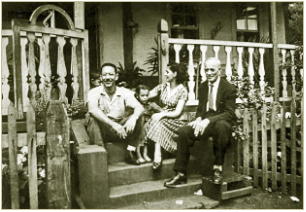
\includegraphics[width=0.6\linewidth]{5/papai+vô joão.png}
\caption{Papai e Vô João nos visitando na sede da fazenda.}
\end{figure}

O primeiro dia de aula numa escola rural tinha que ser invariavelmente dedicado a examinar as unhas, o cabelo e as mãos da criançada.
Piolho, unha suja, pescoço encardido, bicho de pé, nada escapava ao rigoroso escrutínio da brigada sanitária integrada pela minha mãe e pelo casal de tios. 
Na beira do poço, um a um, os alunos iam sendo examinados, lavados e escovados para aprender como deviam se apresentar diante da professora dali em diante. 
Era a primeira lição.

Olhando aqueles meninos atentos e obedientes à minha mãe, que chegavam alegres como uma revoada de andorinhas apesar da dura batalha de todos os dias para vencer os esses e erres, para imitar o talhe impecável da letra da professora, para desvendar os mistérios das divisões e multiplicações, é que eu comecei a achar que essa história de estudo devia ser muito importante mesmo. 
Mas, como esperar que mantivessem os cadernos limpos e organizados como minha mãe queria, se naquele lugar não havia como se livrar da terra nas mãos, nas roupas, na cara, em toda parte? 
Pois não é que eles acabavam conseguindo?  
O ano mal ia a meio e a maioria deles já tinha uma letra redonda e ligeiramente inclinada, como queria a professora, os cadernos encapados, com os parágrafos, margens e vinhetas apropriadamente distribuídos. 
Minha mãe era brava, mas vibrante, entusiasmada e gostava de cantar com eles. 
Também sabia fazer bonitos desenhos na lousa para ilustrar os temas das aulas. Talvez por isso, mais do que atenção, medo ou respeito, o que eu via na expressão daquelas crianças era gratidão, quase adoração.

\begin{figure}[H]
\centering
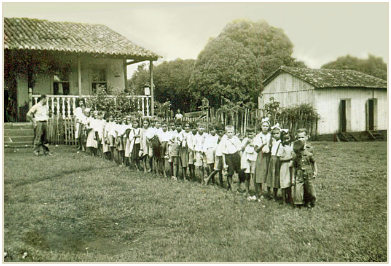
\includegraphics[width=0.6\linewidth]{5/escola.png}
\caption{Os alunos da Fazenda Barrinha, Reginaldo e eu à frente.}
\end{figure}

Foi naquela humilde escolinha rural da Fazenda Barrinha que, sem me dar conta, encantei-me pelo ofício de ensinar.  
E de aprender. 
Era fascinante observar como aquelas crianças, pouco mais que animaizinhos mudos e assustados no primeiro dia de aula, iam se afirmando na sua humanidade, à medida que progrediam nos estudos. 
Pareciam mais alegres, mais confiantes, como se as porteiras do mundo fossem se abrindo diante deles e aquele ingênuo desenho da estrada florida e ensolarada que estampava as capas dos cadernos baratos que o governo lhes fornecia, fosse se materializando diante dos seus olhos.  
Por causa disso, quando eu própria cheguei à idade de frequentar a escola, tinha desse universo a melhor das impressões.
    
A hoje pejorativamente chamada escola reprodutivista, de inspiração cartesiana, tinha o efeito de tornar o mundo muito simples e seguro para as crianças daquele tempo. 
Quem duvidaria que o Brasil fora descoberto por culpa das calmarias na costa africana, se quem o afirmava era Dona Anahyde, minha professora de 4ª série, corpulenta senhora de cabelos vermelhos colados à testa em caprichadas ondinhas e expressão feroz de um guarda penitenciário? 
Aliás, como mamãe proclamava orgulhosamente, fiz meu primário com as melhores professoras do Grupo Escolar, a começar por ela própria, o que significava, principalmente, ter experimentado as mais rígidas disciplinadoras da casa. 
Tenho certeza de que ao cabo da minha vida, a última coisa a se apagar na memória serão os nomes das cidades percorridas pela Estrada de Ferro Central do Brasil, decorados no dia em que Tia Odete, que se gabava de ouvir um alfinete cair na sua silente classe de 3º ano, manteve-me em pé diante do mapa da dita ferrovia durante a tarde toda, porque olhei para trás durante suas explicações, ao ter o cabelo puxado por meu irmão. 
O mundo se dividia, claramente, entre o certo e o errado, o bem e o mal, sem atenuantes, sem nuances, sem relativismos, sem dúvidas. 
Havia uma resposta correta para tudo e a resposta era aquela da professora. 
E os pais estavam de pleno acordo quanto a isso. 
Portanto, podíamos brincar despreocupados no recreio. A vida era previsível e se alguém tivesse cabeça boa para decorar e obedecer a regras e instruções, não havia o que temer. 

Um dia, já Coordenadora Pedagógica de um colégio jesuíta no Piauí, desci aos porões do centenário prédio atrás de livros antigos de aritmética. 
Remexendo as estantes empoeiradas do arquivo, encontrei, caído por detrás delas, um grande caderno de gravuras que o Ministério da Educação distribuía, até meados do século XX, por todas as salas de aula do país e que eu vi, pela primeira vez, na escola da Barrinha.  
Era o material de apoio utilizado nas aulas de redação, numa prática anunciada como ``composição à vista de uma gravura'' e que podia ser, alternadamente, uma descrição ou uma narração. 
Consistia numa sucessão de estampas ingênuas, exibindo crianças e animaizinhos felizes em campos floridos, árvores frondosas, casinhas aninhadas entre montanhas, nuvens brancas e gorduchas por sobre as quais brilhavam invariavelmente os raios amarelos do sol. 
Judiciosamente, a professora dava o começo, escrito em letras caprichadas na lousa: ``Era uma linda manhã de primavera\dots''. 
As reticências eram a deixa para que nós, os alunos, fôssemos em frente. 
Maravilhada, corri para exibir o achado à minha colega de Coordenação, Jovina, que tinha mais ou menos a minha idade e, portanto, devia ter cursado o primário na mesma época.  
Paulista eu, piauiense ela, descobrimos, às gargalhadas, que a distância de alguns milhares de quilômetros não impedira a inacreditável coincidência de adjetivos, advérbios e frases feitas inspiradas pelas tais gravuras e que, usados em profusão, garantiram para ambas a aprovação com louvor naquela matéria. Assim que passou o surto de hilaridade, minha colega comentou: 

{\itshape``-- Hoje a gente ri, mas me diga, aqui na escola, quando é preciso redigir um discurso, um ofício, um requerimento ou até uma simples comunicação, é atrás de nós duas que eles vêm, é, ou não é?''}
\chapter{}
Fui, ao longo da minha vida escolar, uma boa aluna. 
Não porque fosse uma grande estudiosa, mas sim, porque aprendi a gostar de ler. Meu pai tinha o hábito de, logo depois de retirada a louça do jantar, abrir o jornal sobre a mesa e comentar em voz alta as notícias do dia. 
Parecia tirar um grande prazer disso, de tal forma que comecei a encarapitar-me junto dele, querendo partilhar do ritual, embora fosse ainda muito pequena para entender qualquer coisa. Achando graça, papai começou a soletrar comigo o título do jornal até que “Folha da Manhã” foi a primeira coisa que li na vida, com dígrafos, til e tudo. 
Com o passar dos anos, de alguma maneira devo ter percebido que nos livros estavam as respostas para o meu precoce interesse pelas pessoas e pela vida em geral. 
Além disso, logo ficou claro para mim que a leitura proporcionava um agradabilíssimo e rendoso disfarce para a minha dificuldade de memorizar, deficiência preocupante na vigência de uma prática escolar em que a promoção dependia exclusivamente do talento do aluno para reproduzir com absoluta fidelidade o que ensinavam os livros ou o professor. 
Descobri que só guardava o que conseguia entender, digerir e devolver com minhas próprias palavras e a leitura foi a grande responsável pela facilidade com que passei a realizar tais operações. 

Acho que o ponto alto da minha estratégia para ocultar dos professores a incapacidade de decorar aconteceu quando eu cursava a oitava série, no dia em que a mais temida professora do Colégio, D. Cidinha, professora de História, chamou-me para entregar uma prova e perscrutando-me miudamente o rosto, disse:
 
{\itshape``-Teresa, dei-lhe uma nota oito, porque sua narração da revolta pela libertação da Grécia não só está bem redigida, como satisfatoriamente fiel; entretanto, como você omitiu datas e nomes, é verdade que ela se ajustaria à maior parte das revoluções da História. Na pior das hipóteses, você parece ter aprendido bastante sobre a dinâmica dos movimentos revolucionários.''}

Lembrei-me deste fato quando me tornei eu própria uma professora de História e passei a inaugurar meus cursos comunicando aos espantados alunos que naquele ano experimentariam uma novidade: uma professora de História desmemoriada, incapaz de guardar datas e nomes, mas muito interessada nos porquês da História e, principalmente no uso que poderíamos fazer deles para as nossas vidas. 

Mas, ai de mim, nas então pretensiosamente chamadas “ciências exatas”, com relevo especial para a Matemática, nenhuma estratégia funcionava. 
Tudo me parecia de um autoritarismo monolítico, intolerável, com suas regras, axiomas e princípios. 
Enquanto estudei aritmética saí-me até bem, pois, como lembrou um nosso cronista, acho que Rubem Braga, havia enredo na coisa. 
Havia ética que convidava à solidariedade no esforço de encontrar o troco exato ou de repartir terrenos, laranjas ou bolas de gude de modo que o resultado fosse perfeitamente aceitável para os interessados. 
Quando, porém, ao ingressar no ginásio, fui conduzida por aquele que seria meu único professor da matéria a partir daí, aos tenebrosos domínios da Álgebra, uma parte do meu cérebro entrou em colapso e pareceu soçobrar no oceano escuro da ignorância. 
Para sempre. 
Tornei-me, desde então, incapaz de pensar a vida em números. 
Avessa a medir e contar, fosse lá o que fosse. Mistério considerado insondável por quantos se detiveram a analisar o problema. 

Aquele professor era proclamado um gênio por toda a cidade. 
Muito magro e agitado, avental imaculadamente branco, cheirando a lavanda e cigarro, ele entrava na classe já ditando a lição e escrevendo compulsivamente no quadro negro. Como hieróglifos numa tumba egípcia, intermináveis equações, trinômios, polinômios iam se estampando em ritmo frenético por toda a lousa e, quando esta se esgotava, pelas paredes. 
O giz ia se despedaçando entre os dedos nervosos e espalhando-se pelo chão. 
A intervalos, ele catava os toquinhos e despejava-os numa caixa. 
Tinha uso para eles: atirava-os na cabeça dos distraídos. 
Eu estava entre os seus alvos preferidos. Ao lado da escola, uma imensa paineira lançava ao vento delicados flocos que entravam pela janela da sala e flutuavam como bailarinas minúsculas diante dos meus olhos enlevados.  
Desse devaneio me tirava a voz aguda do professor e o concomitante estalinho do toco de giz sobre a testa:

{\itshape“- {\large\bfseries D o n a T e r e s a F i l p i}, depois não sabe por que não entende   Matemática, não é?”}

Por vias indiretas, devo muito a esse professor. 
Não sei por que, encasquetei com a idéia de encaminhar-me para Medicina quando cheguei ao curso médio ou Colegial, como era chamado então. 
Para tanto, matriculei-me no Científico, opção que enfatizava as Ciências Exatas, com aulas diárias e reforçadas de Matemática. 
Ao dar comigo na classe de primeiro ano, um esgazeado Sr. Ulysses, era assim que ele se chamava, abandonou a sala e dirigindo-se a um telefone ligou para minha mãe exigindo que ela providenciasse a minha imediata transferência para o curso Clássico, que preparava para as faculdades de Línguas e Ciências Humanas. 
Minha mãe obedeceu no ato. Odiei-o por isso e por muito tempo julguei-me frustrada em minha vocação. 
Tornei-me então, educadora. 
Muito tempo depois, haveria de ter um contato mais próximo com a vida de um médico quando, durante a recuperação de uma fratura no pé, trabalhei com meu irmão João na sua clínica de ortopedia. 
Só então é que, no íntimo, agradeci fervorosamente àquele impaciente professor. Jamais teria experimentado pela rotina médica a paixão que me despertou a batalha diária nas salas de aula. 
E mais, a lembrança do martírio que esse professor e eu mutuamente nos infligimos, me orientou a empreender uma revolução no ensino de Matemática do colégio que eu coordenei. 
Jamais consegui aceitar que uma ciência que nasceu para favorecer a harmonia e a ética, educando os homens para a honestidade e para a civilidade, fosse tão desvirtuada por uma pedagogia arbitrária e pretensamente neutra, a pretexto de ser “científica”. 

A baixa remuneração dos professores, uma triste recorrência na história da educação brasileira, sempre trouxe como efeito, entre tantos outros, a absurda carga horária assumida pela maioria deles e que fazia com que, à semelhança do que me ocorreu com a Matemática, os alunos, numa determinada disciplina, tivessem o mesmo professor por anos a fio. 
Havia deles que ministravam aulas desde o início do primeiro grau até o fim do segundo. 
Quando eram bons, isto era uma sorte incrível na mediocridade reinante. 
Mas, se eram deficientes, o aluno ficava lesado para todo o sempre. 
Aconteceu-me com Geografia, além de Matemática. Ainda hoje ostento uma dificuldade irritante, verdadeiramente limítrofe, para me orientar no espaço. 
Mas, em Português, em compensação, tive, por seis anos consecutivos, um professor maravilhoso que se sustentara na faculdade interpretando radionovelas e que adorava ler para nós. 
Aprendi a língua como quem aprendesse música. 
Nunca soube, como continuo a não saber, regras gramaticais, porque ele não nos aborrecia com isso. 
Aprendi a escrever lendo com ele gente que escrevia bem.  
E ouvindo aquela voz sonora e expressiva realçando o estilo e a elegância do autor. 
Meu velho e querido Professor Jurandyr. Muito aprendi também com Dona Elisa, sobrinha de Mario de Andrade, por curtos anos minha professora de francês e que falava de autores e livros como quem descrevesse delícias culinárias. 
Salivando gulosamente. 
E provocando, em quem a ouvia, uma fome danada de ler. 
E Dona Olga, poetisa de parnasianos versos, uma típica sobrevivente de tempos machadianos, cujo pai tinha sido amigo muito chegado de Ruy Barbosa. 
Anacrônica dama, capaz de exigir dos seus aluninhos, como lição de casa, doze sinônimos para o adjetivo cinzento. 
Que Deus abençoe a todos, quanto lhes devo!

\chapter{}

\begin{figure}[H]
\hfill
\centering
\begin{subfigure}[h]{0.4\linewidth}
    \centering
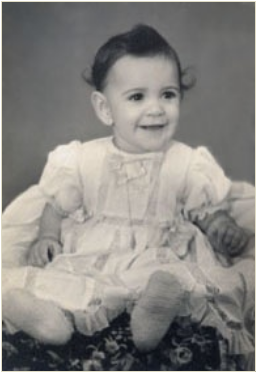
\includegraphics[width=\linewidth]{7/batismo.png}
\caption{Batismo}
\end{subfigure}
\hfill
\begin{subfigure}[h]{0.4\linewidth}
    \centering
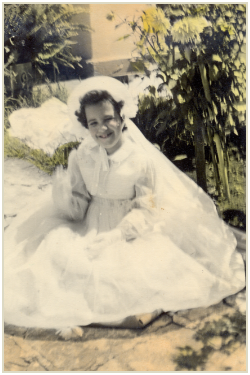
\includegraphics[width=1\linewidth]{7/1a-comunhão.png}
\caption{Primeira Comunhão}
\end{subfigure}
\end{figure}

Fui batizada, crismada, fiz primeira comunhão, novenas, ganhei indulgências, decorei os dez mandamentos, os sete pecados capitais, jurei ser católica apostólica romana e abjurei do demônio ainda em tenra infância, sem ter a menor idéia de quem eram os romanos, os católicos ou o demônio, ou do que fosse pecado. 
Rezava para o Santo Anjo todas as noites e fazia penitência após a confissão. 
Adulta, morei com freiras, trabalhei com padres e casei no religioso. 
Após tudo isso, sou uma católica bissexta que crê firmemente em Deus e muito pouco na Igreja. 
Sou grata a Ele por me ter concedido participação nesse imenso projeto que é a Vida e me inquieta a constatação, nessa altura da minha existência, de que recebi muito mais do que dei. 
Quando leio ou ouço dizer que a Vida não é um dom ou uma graça, mas um caos produzido por uma energia errática e perversa, lembro-me da parábola contada por um jesuíta sobre a formiga que, caminhando com dificuldade sobre uma imensa toalha de renda de fino lavor, bradava contra o desastrado e incompetente artesão que a teceu, maldizendo os buracos onde suas patinhas se enredavam.

Lá pelo meio do meu sexto ano de vida, em sinal de gratidão a Deus pela cura da nefrite que me vitimara, vestiram-me de anjo para acompanhar o pálio de Corpus Christi, numa das muitas procissões que o Vigário da Matriz organizava ao longo do ano. 
Halo dourado cingindo a cabeça, encimado por uma estrela, imensas asas de penas de ganso tingidas, envergando uma camisola longa de tafetá, toda em amarelo radiante, lá fui eu rebocada pela Vó Didi. 

A escolha da cor amarela tinha a ver com o fato de que minha avó era a zeladora do altar de São José, posição de destaque na hierarquia da irmandade do venerável santo, irmandade essa identificada pela fita amarela que suas participantes traziam ao pescoço. 
Na queda de braço entre as tias, irmãs de papai e a avó para decidir de que cor seria o anjo, mamãe optou por dar vitória à D. Didi. 
Talvez porque a cor da fita que identificava a irmandade das tias fosse vermelha. 
Elas pertenciam à irmandade do Sagrado Coração de Jesus, maior e mais importante do que a de São José, pelo menos me parecia, pois a fita que ostentavam era debruada em dourado e o andor que carregavam, sempre maior e mais enfeitado que os outros, saia na parte central da procissão. 

Uma sobrevivência medieval, as irmandades, por ocasião das festas religiosas, assumiam feição de torcidas organizadas em favor deste ou daquele santo padroeiro. Havia a dos Congregados Marianos, para os homens jovens ou solteiros; os mais velhos integravam os Irmãos do Santíssimo e tinham a missão de abrir solenemente as procissões portando grandes tocheiros e envergando uma opa cor de púrpura; as senhoritas casadoiras reuniam-se sob o estandarte das Filhas de Maria, imaculadamente vestidas de branco e ostentando fitas de tafetá azul celeste sobre o peito. 
Ser congregado mariano ou filha de Maria, para as famílias da cidade, era garantia de bom comportamento e pré-requisito de importância no currículo de qualquer jovem postulante ao casamento. 

\begin{figure}[H]
\centering
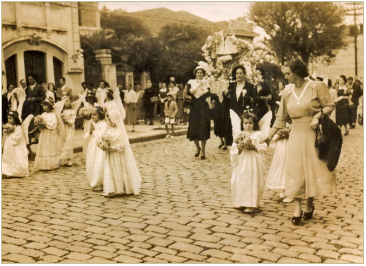
\includegraphics[width=0.8\textwidth]{7/procissão.png}
\caption{Procissão em Araraquara: Tia Angelina, a matriarca dos Ópice, segura a alça esquerda do andor}
\end{figure}

Pois bem, na tal procissão em que eu deveria desfilar de anjo, sabe-se lá por que, o senhor vigário, na última hora, decretou a dissolução da corte celestial e determinou que cada irmandade arcasse com o trabalho de conduzir e vigiar seus querubins. 
Desconfio que não estávamos parecendo suficientemente angelicais aos olhos do velho e cansado sacerdote. 
Ou, talvez, sua escassa paciência tenha se esgotado com a encarniçada disputa entre as representantes das várias facções para decidir se os anjos sairiam por ordem de tamanho, de beleza ou de importância da congregação representada. 

De tudo quanto pode ser reunido sob o rótulo de Religião, lembro-me bem do cheiro que pairava no interior da Matriz, sobretudo nas missas das seis da manhã em que eu acompanhava as tias ou a Vó Didi para me livrar logo da obrigação dominical. 
Era o mesmo cheiro que impregnava o missal, a mantilha e o traje negro de todas elas: uma mistura de flores murchas, cera de vela e um leve odor de mofo misturado à fumaça do incenso do turíbulo que o sonolento coroinha balançava para lá e para cá, hipnotizando meus olhos mal acordados.  
E de um silêncio de mistério que enchia a nave mal iluminada pela primeira claridade da manhã, docemente quebrado pelo cicio dos lábios murchos das velhas beatas no afã de acompanhar o monótono latinório do velho pároco, ainda mais incompreensível porque rouco, baixo e apressado. 
De tempos em tempos, o tilintar da campainha que o coroinha sacudia, reagindo a um cutucão do padre, alertava para a aproximação da parte principal da missa, a comunhão, à qual se seguiria, pouco depois, o esperado ``Ite missa est!''.

A Igreja Matriz da cidade era pequena, mas bem proporcionada. 
No seu interior, como era moda na época, pinturas de \textit{``trompe l’oeil''} imitavam volutas, sancas e florões e anjos e santos habitavam céus azuis cravejados de estrelinhas douradas. 
As paredes exibiam painéis e colunas fingindo mármores preciosos de Carrara. 
O altar-mor era de madeira torneada, pintado de branco e azul e debruado em dourado. 
Uma decoração, enfim, toda compatível com o Olimpo cristão constelado no imaginário popular. 
Tinha lá sua graça.
Um dia, apresentou-se na missa das dez, a mais importante, o clérigo que vinha para finalmente substituir o nosso já muito adoentado vigário, Padre Colturato. 
Bonitão, moderno, bom orador, Padre Orlando chegou causando \textit{``frisson''}. 
E implicando de saída com a velha igreja. 
Araraquara merecia coisa muito melhor, bradou ele do púlpito. 
E logo deu início a campanhas, quermesses e promoções para arrecadação de fundos. Seria uma construção monumental, digna da fé do rebanho araraquarense. 
As opiniões dividiam-se pró e contra a modernização da Matriz. Mas a oratória do novo vigário e o trabalho incessante dos cupins venceram a parada. 
A Matriz seria derrubada. 
A decisão veio a público no final da Quaresma, um pouco antes da Semana Santa.

Na Sexta-Feira, dia em que se dava o ápice das comemorações do período, acontecia o Encontro, evento noturno em que duas procissões iluminadas por velas e partindo de pontos opostos da cidade traziam até o Largo da Câmara, uma, a imagem de Jesus morto em seu ataúde, e outra, a de Nossa Senhora das Dores, com seu manto roxo, suas lágrimas de sangue e o punhal de prata cravado no peito. 
E o rosto emoldurado pelos cachos da Tia Angelina, a matriarca dos Ópice, que os havia cortado e doado à santa no cumprimento de uma promessa. 
Eu torcia sempre para que meus pais escolhessem acompanhar a primeira procissão, porque nela ia a Verônica, uma mulher oculta em longo e negro véu, que em cada esquina do trajeto subia num banquinho e, entoando um canto pungente, desenrolava um pano branco onde se via impresso o rosto martirizado do Cristo. 
Nela iam ainda as matracas, instrumentos medievais que serviam para alertar para a aproximação do féretro, feitos de uma aldrava de metal que batia contra uma prancha de madeira, produzindo um som cavo de ossos chacoalhando. Aquela encenação carregada de dramaticidade, à luz oscilante das velas, estampava na fisionomia das pessoas qualquer coisa de fantasmagórico. Até as feições do pessoal de casa me pareciam sobrenaturais. 
A impressão era tamanha que ainda sou capaz de ouvir as vozes misturadas de homens e mulheres cantando e implorando: \textit{``Pela Virgem Dolorosa, Nossa Mãe tão piedosa, perdoai, ó meu Jesus; perdoai, ó meu Jesus!''}.

Pois bem, naquela sexta-feira, após o encontro e incorporadas, as duas procissões seguiram para o desfecho na Igreja Matriz, onde acontecia a Hora de Guarda, cerimônia em que a imagem do corpo do Senhor era velada pelos fiéis até o alvorecer da Aleluia. 
Ia o culto a meio, quando um estrondo de fim de mundo rasgou o céu e um aguaceiro daqueles desabou. 
Entretido na procissão, o povo não se deu conta da tempestade que se aproximava. 
O vento invadiu a nave sibilando, sacudindo e batendo portas e janelas. 
O grande lustre que pendia da cúpula da Igreja desandou num balanço alucinado e acabou despencando, acompanhado de um dos vitrais que, após violento estalo, veio igualmente estilhaçar-se no chão. 
À chuva de cacos seguiu-se uma torrente de água que inundou tudo. 
Espavorida, a multidão arremeteu para as saídas, esquecendo-se do morto sagrado que lá ficou com sua Santa Mãe entre os escombros. 
Corremos nós também, rua abaixo, protegidos apenas pelos \textit{``Santa Clara!''} que a minha mãe invocava entre sinais da cruz, a cada vez que um raio explodia sobre nossas cabeças. 
Chegamos em casa molhados dos cabelos aos sapatos. 
A tempo de descobrir que parte do nosso telhado jazia espatifado sobre a calçada e generosas goteiras, caindo através do forro de madeira, haviam transformado nossos quartos em lagoas. 
Dormimos papai, mamãe, Reginaldo e eu amontoados num pedaço da sala que se conservara seco.

Por muito tempo, Padre Orlando teve que ouvir que aquela Sexta-Feira Santa tinha sido o castigo merecido pela nefasta decisão de derrubar a velha Matriz. 
Verdade ou não, o fato é que o pretensioso projeto que aos poucos foi se materializando no lugar da humilde igrejinha nunca foi terminado. 
O solo poroso não lhe suportou o peso e a construção rachou ameaçadoramente quando o trabalho ainda nem chegara à metade. 
E até hoje ela lá está, inacabada, grandalhona e deforme como se mutilada por uma praga. 
\textit{``-- Monumento à arrogância daquele padre de meia-tigela''}, esconjurou minha mãe até o fim da vida. 
O desprezo veio se somar à aversão quando ela soube, poucos meses depois, que a reverendíssima figura tinha abandonado a batina e fugido com a bela filha do confeiteiro.

Adulta, trabalhei com jesuítas. Revisitei lembranças, cauterizei feridas que o desencanto abriu na minha claudicante fé, fortaleci algumas intuições apenas pressentidas anteriormente, mas também vi evaporar outras que até então me traziam consolo. Aí comecei uma lenta e difícil jornada de descoberta de um caminho para um Deus que eu pressinto, não alcanço e pelo qual anseio, como todos os outros, mesmo aqueles que O desacreditam.  Ensinou um rabino que, para negar Deus, é preciso que haja um Deus a ser negado. É preciso descobrir de que Deus somos ateus. E encontrar o Deus verdadeiro que, dizem, aguarda-nos lá onde nos é mais difícil procurá-lo: no mais profundo de nós mesmos. 
\chapter{}
Nas férias, Tio Totó, o irmão mais velho do papai que morava na fazenda, vinha buscar as filhas na casa das tias, onde elas se hospedavam no período escolar.
De cambulhada, levava-nos a mim e ao Reginaldo para fazer companhia às primas.
Era uma alegria. 
Eu adorava a fazenda e até hoje minhas inclinações e preferências, em muitos aspectos da vida, têm suas raízes naqueles dias passados na Barrinha, na Pedra Branca e na Fazendinha. 

Tio Totó era um fazendeiro remanescente dos tempos em que o dono da terra era patrão, médico e juiz, com autoridade civil e criminal sobre seus colonos. 
De manhãzinha, a fila se formava na porta da cozinha e o atendimento começava: era conselho para um, sermão para outro, remédio para o filho daquele outro, curativo, injeção, encomendas para serem levadas mais tarde à cidade, conciliação das desavenças e por aí afora. 
Ao lado, silenciosa e atenta, Tia Albina, mulher, companheira e assistente, ia organizando a fila, desinfetando seringas, ajudando nos curativos, anotando os pedidos. 
A maioria era compadre, seja porque o casal lhes apadrinhara o casamento ou um dos filhos. Terminada a sessão, Tio Totó tomava mais um cafezinho na beira do fogão e saía para a roça. 
Quase nunca se dando ao trabalho de abrir a porteira. 
Preferia por as mãos sobre o mourão da cerca e agilmente pular sobre o arame, vigoroso e elástico. 
Tínhamos por ele o maior respeito, senão medo, que a Tia Albina cuidava de alimentar: \textit{``-- Olhe que quando o Totó chegar, o pau vai comer!''}. Era água na fervura.
Porque o tio era bruto e quando ficava bravo não media nem palavras, nem gestos. 
Num prenúncio aterrador do que estava por vir, seu olho estrábico metia-se de tal forma para dentro que só lhe víamos o branco da esclerótica. 
Mas, também sabia ser divertido e nos levava a passear na sua caminhonete, recolher prendas nas fazendas vizinhas para a quermesse do padre, ou tomar sorvete na cidadezinha próxima, sua amada Boa Esperança. 
Pela vida inteira, até morrer, Boa Esperança, sua terra natal, ocupou o centro das suas preocupações, sobrepondo-se a quaisquer outras, incluídos aí mulher, filhos e negócios. 
Nunca desistiu de colocar sua cidade no mapa do desenvolvimento paulista e para tanto se elegeu prefeito por duas vezes e vereador outras tantas. 
Os conchavos políticos eram realizados ali mesmo no terreiro e com uma característica \textit{sui generis}: os participantes eram obrigados a ficar de cócoras porque seu líder, meu tio, preferia essa posição para, didaticamente, expor suas estratégias, desenhando-as com um graveto na poeira do chão.

\begin{figure}[H]
\centering
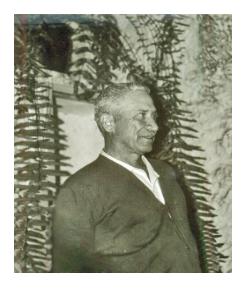
\includegraphics[width = 0.6\linewidth]{8/tio-totó.png}
\caption{Tio Totó.}
\end{figure}

Tia Albina trazia em si toda a sabedoria intuitiva e matreira da nossa gente cabocla. 
Ainda que usualmente se mantivesse quieta e passiva à retaguarda do companheiro, tinha uma luz própria que só percebia quem lhe ouvisse as observações cochichadas por entre o riso silencioso e sacudido. 
Que observadora implacável era ela! Nada lhe escapava.  
Gordinha, baixinha, sabia, contudo, irradiar majestade quando andava entre seus súditos na colônia. 
Sem nem levantar a voz.  
Vestidos invariavelmente ``ramadinhos'', como ela gostava, avental e chinelinhas, cabelo preso em coque na nuca, mal raiava o dia e lá estava ela no comando das tarefas domésticas, pois que seu amo e senhor queria tudo a tempo e a hora, embora fosse ele próprio completamente imprevisível, a ponto de que, na família, ``totozão'' virou epíteto para os eternamente fora de hora.  
O tio não tinha hora para coisa alguma e podia aparecer com um bando de correligionários ou amigos para almoçar sem nenhum aviso prévio. 
Disso resultou que ninguém, como Tia Albina, desenvolveu tamanha competência em produzir refeições saborosas em tempo recorde. Havia uma janelinha estratégica na cozinha, de onde se via a estrada da fazenda. 
Assim que divisava um carro diferente acompanhando o do tio, Tia Albina saia porta afora, agarrava certeira o primeiro frango que lhe passasse na frente e quando a visita sentava para conversar, já o aroma do seu insuperável franguinho frito inundava a casa toda. 
Mais uma corridinha à horta e o banquete estava pronto! Com a carinha mais sossegada do mundo, ela sorria aos elogios:
\textit{``-- Que nada''}, dizia, \textit{``comidinha simples da roça. Aposto que na cidade vocês comem coisa muito melhor''}.

\begin{figure}[H]
\centering
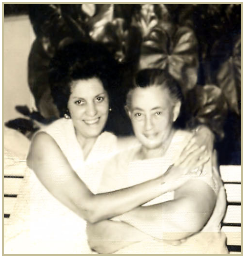
\includegraphics[width = 0.6\linewidth]{8/tia-albina.png}
\caption{Tia Albina abraçada por mamãe.}
\end{figure}

Muitas vezes me ocorreu que minhas primas perderam muito por não terem sido criadas pela mãe.
A mais velha foi-lhe tirada muito cedo e entregue à avó Teresa.
Parece que era outro costume trazido da Itália, o de levar os primogênitos para serem educados na casa dos avós paternos.
Em casa, a tradição foi derrotada pela resistência feroz e intransponível da minha mãe.
Ainda bem.
Tia Albina, porém, curvou-se à vontade do marido.
Aos poucos, as outras três lhe foram sendo tomadas quando chegavam à idade de freqüentar a escola.
Só lhe deixaram o temporão, Reginaldo Antônio, que contrariando os prognósticos de que criado na roça nunca seria alguém, é hoje um bem sucedido homem de negócios e um ser humano por quem tenho carinho e muita admiração.
Se mágoa restou em minha tia pelas filhas que lhe foram subtraídas, nunca demonstrou.
Mas acho que teria sido, sob muitos aspectos, uma mãe intuitivamente criativa.
Ensinou-nos a brincar com sucata, boizinhos de bucha, a fazer carrinhos de carretéis vazios.
Com caquinhos de louça nos fez imaginar ricas baixelas nas brincadeiras de casinha.
Com ela, aprendemos a fazer bruxinhas de pano, recortar figuras de moças e rapazes de revistas velhas para representar histórias que nos distraiam por horas seguidas.
De outras vezes, riscava flores ingênuas em pedaços de sacos alvejados e nos ensinava a bordar com linhas coloridas.
Prontos os bordados, ela fazia bicos de crochê à volta, transformando-os em toalhinhas que fazia questão de engomar para com elas enfeitar toda a casa.
Franqueava-nos também um maravilhoso baú onde guardava sapatos e vestidos antigos e nos dava, para acompanhar, sobras de pó de arroz \textit{Lady}, \textit{``rouge''} e toquinhos de batom.
Divertia-se vendo-nos encarnar madames, atrizes e princesas, convencidas de que estávamos deslumbrantes! Do bolso do avental.
sacava inesgotáveis moedinhas com que corríamos para comprar pirulitos, suspiros e ladrilhos de goiabada na vendinha do povoado.
E quando fazia pão, punha-nos à volta da mesa e nos dava pedaços de massa para que cada um fizesse seu próprio pãozinho, com a forma que a imaginação sugerisse.
Depois, punha-os para assar e os comíamos no lanche com queijo caseiro derretido na brasa.


Da casa da Tia Albina íamos com frequência para a da Tia Yolanda, que sempre morou não muito longe da cunhada e com ela dividia a tarefa de nos receber nas férias.
Já esta outra tia, a ama e senhora primeiro da Barrinha e depois da Fazendinha, como boa Filpi, tinha o gênio instável da raça.
Adorava crianças.
Cozinhava divinamente, empanturrava-nos de doces e bolinhos até a náusea.
Divertia-se com nossas traquinagens, mas nunca sabíamos quando sua braveza viria à tona, o que nos punha um tanto ressabiados.
Diziam que ela era a mais brava das irmãs.
Durante o tempo em que moramos, Reginaldo, mamãe e eu na casa dela na Barrinha, Reginaldo, que era muito levado, andou experimentando aqui e ali amostras do seu famoso temperamento.
Já eu não me lembro de lhe ter ouvido uma palavra mais áspera.
Nem mesmo quando ela encontrou as preciosas botas de montaria do seu Tio Aniello entupidas de massa crua, fermentada e embolorada.
Tio Aniello era meio parente do Vô Reginaldo, um senhor muito elegante e educado, casado com uma francesa e que vinha anualmente à fazenda para caçar codornas.
Brincando no quarto dos arreios, achei que as botas dele davam um ótimo forno para assar o pão das minhas bonecas e acabei esquecendo tudo lá, apodrecendo por dias e dias.

Tia Yolanda não teve filhos.
Talvez por isso tivesse menos jeito que a Tia Albina para lidar com os sobrinhos.
Ou talvez tivesse menos motivos para ser feliz.
Entre as irmãs, ela teve a educação mais cuidada.
Como era a filha mais velha, viveu a adolescência nos tempos de prosperidade do Vovô.
E, para aprimorar sua educação, chegou a morar por algum tempo com um irmão da Vó Teresa, um tal Tio João, muito abastado, casado com uma professora de maneiras refinadas que ensinou à Tia Yolanda modos e gostos de madame.
E minha tia era vocacionada para a coisa.
Atestava-o gesto característico de erguer delicadamente o indicador e o mindinho junto à face, quando se punha a contar um caso.
Porém Tio Zé, o marido, nunca deu muita sorte na vida.
Na verdade, nada do que lhe era confiado ia adiante.
Imagino até que teriam passado dificuldades se não morassem no campo que lhes provia as necessidades mais básicas.
Hoje, relembrando as sedes simples de ambas as fazendas, dou-me conta da quase penúria em que viviam.
O enxoval era de algodãozinho alvejado, áspero e imaculadamente branco.
Igualmente brancas eram as capas do sofá improvisado e das poltronas.
Com bicos de crochê e bordados, ela disfarçava a pobreza tecido.
Mas era a limpeza o grande trunfo e o grande luxo daquela decoração franciscana.
Meu Deus, como Tia Yolanda se devotou à limpeza, pela vida toda! Ainda que Os Filpi e os Vitta parecessem disputar o campeonato mundial do asseio doméstico, ninguém, para mim, batia Tia Yolanda na competência de fazer emanar das roupas, da casa, das louças, da mobília, aquele aroma inesquecível de água pura, de sol, de limpeza.
Ambas aquelas moradas humildes, a da Barrinha e a da Fazendinha, sempre produziram em mim o mesmo efeito de paz e integração com a vida.
No silêncio da tarde, o perfume das flores simples, do pé de jasmim, do capim-cidreira, da moita de arruda, trazido pelo vento que entrava pelas janelas fazendo esvoaçar as cortinas alvas, envolvia-me numa sensação de felicidade e completude que pelo resto da vida eu tento debalde reconstituir nas casas onde moro.
Faltam-me, entretanto, as grandes vascas de lavar roupa que a tia emoldurava de rosinhas trepadeiras e os varais batidos de luz onde os lençóis e toalhas panejavam contra o céu, o branco azulado de anil quase cegando a gente.
Faltam-me também suas mãos hábeis e fortes, contidas e suavizadas pelas maneiras fidalgas, lavando, esfregando, fervendo, areando, engomando, eternamente, incansavelmente.

\begin{figure}[H]
\centering
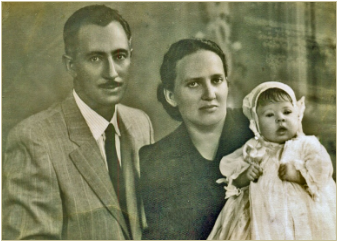
\includegraphics[width = 0.8\linewidth]{8/zé+yolanda.png}
\caption{Tio Zé e Tia Yolanda com minha prima Laura.}
\end{figure}

Essa atmosfera meio rural que leva as pessoas a acharem que as casas que eu arrumo têm um jeito de fazenda ou de casa de avó, devo-a às lembranças que ficaram desses lugares da minha infância.
Da nostalgia daquela estética ingênua das paredes brancas, do chão de tijolo e tábuas lavadas, das toalhinhas de crochê, dos canteiros de Maria-sem-vergonha, das cercas e portões enroscados de melindro e flor-de-São-João.
Mas, não seria justo deixar de mencionar a contribuição que me veio, também intensa, da casa das tias, irmãs do meu pai e da minha avó Didi, porque nelas eu andava quase diariamente e ambas, ainda que urbanas, conservavam o mesmo frescor singelo, a honesta simplicidade que tanto me encantava naquelas outras, as dos tios da fazenda.


A casa da Vó Didi, a primeira de que me lembro antes que Tia Maria Angelina se tornasse moça e começasse a impor seu gosto moderno e mais sofisticado, acachapava-se, baixinha e esparramada, numa esquina do Largo da Câmara.
Era daquelas de janela na rua, típica construção popular de inspiração portuguesa, tão comum nas antigas cidades brasileiras.
De precioso só mesmo a imensa mangueira que sombreava os fundos do grande quintal e o jardim lateral, o “ai-Jesus” da vovó, onde se misturavam em deliciosa confusão flores, folhagens, hortaliças, legumes, ervas de tempero e mezinhas.
Dentro, nada de sofás ou tapetes.
Motivo de orgulho eram a sala de jantar completa, a cômoda e dois criados-mudos de jacarandá cheiroso e finamente entalhado, fabricados na Mobiliadora do Tio José.
As panelas brilhavam como prata polida.
Assim como o chão encerado de joelhos e lustrado no escovão.
O cheiro que vinha do fogão à lenha era, segundo meu pai, tal como o sabor que ele prenunciava, inimitável.
Até hoje, nenhuma de nós, descendentes, conseguiu reproduzir nem um, nem outro, embora os ingredientes fossem pobres e a comida feita às pressas, entre uma e outra das muitas atividades da atribulada Didi
Para o molho de macarrão, exigente em calma e capricho, de bom grado ela passava o bastão ao marido, que ela não tinha tempo e nem paciência para tanta firula.

\begin{figure}[H]
\centering
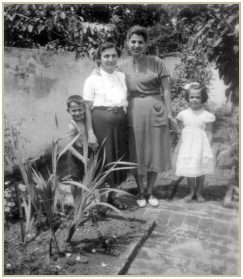
\includegraphics[width = 0.6\linewidth]{8/no-jardim.png}
\caption{No jardim da casa da Vó Didi.}
\end{figure}

Já a casa das tias, na Avenida D.Pedro II, embora externamente aparentasse certa elegância citadina com suas janelas altas e o porão que lhe elevava o pé direito, internamente parecia e funcionava como uma casa de fazenda.
A grande copa de assoalho lavado era o coração da residência.
Ali se passava roupa, faziam-se os trabalhos de agulha e recebiam-se as visitas dos mais chegados para o cafezinho coado sempre em duas versões: uma mais forte para os homens que o tomavam puro e outra mais fraca, para comer com bolos ou biscoitos, para as mulheres.
Vó Tereza, enquanto viveu, sentava-se rente à porta que abria para a cozinha.
Dali tinha um olho nas panelas que a Tia Glória ajudava a administrar e outro na engomação das roupas ou no cerzido das meias, o crochê, o bordado e a costura, a cargo da Tia Neta ou da Tia Imaculada.
Dos cercados do quintal vinham o frango, a galinha gorda, mortos e depenados na hora, os ovos frescos, o leitãozinho e, perto do Natal, até o cabrito.
E, da horta, o tomate, as verduras e temperos.
Pouco frequentávamos a sala de visitas.
Era vedada às crianças, sempre fechada, só aberta para a limpeza diária e para as visitas de cerimônia, pois guardava o que sobrou dos tempos de fausto do café: porcelanas, cristais e o grande piano alemão que ainda ostentava os castiçais de bronze fixados de cada lado do suporte para partituras.
Mas, dos quartos, dos lençóis brancos e dos travesseiros em que nos aninhávamos nas noites de festa, quando o sono nos vencia, emanava aquele mesmo cheiro de sol e água pura que me transportava, nos sonhos, de volta para a Barrinha, para a Fazendinha, para a Pedra Branca.

\begin{figure}[H]
\centering
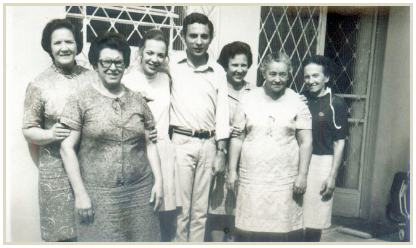
\includegraphics[width = 0.8\linewidth]{8/tias-no-noivado.png}
\caption{Ladeando Paulo e a mim, a partir da esquerda, as tias Glória, Imaculada, Antonieta, Albina e Yolanda, no dia do nosso noivado.}
\end{figure}

Essas mulheres da minha infância, tias e avós, suas casas, os perfumes que evolavam dos seus fogões, das suas hortas e jardins, dos assoalhos lavados, dos lençóis e toalhas que me envolviam, a quietude mansa que espalhavam ao seu redor quando, findo o trabalho do dia, sentavam-se para bordar, costurar, crochetar, alimentavam em mim a crença mágica de que detinham o poder de pôr em harmonia todo o Universo.
De noite, quando deitava minha cabeça naqueles travesseiros recheados de paina cheirosa que elas pacientemente descaroçavam e desfiavam, invadia-me a certeza tranquilizadora de que não só a casa, mas o mundo todo estava limpo e arrumado, na mais absoluta paz.
Então, eu me abandonava ao sono, confiante e feliz.
Se hoje, mesmo sob protestos, tento conservar as tradições que delas me vieram, é com certeza na ilusão de reeditar um pouco desse feitiço para os que não tiveram a sorte de experimentá-lo.

\chapter{}
Dos irmãos Filpi, apenas três cursaram faculdade: Tio Ângelo, o mais velho e Tio Zico, o mais novo, diplomados em Medicina e Tio Bepe, que se tornou farmacêutico.
Papai e Tio Totó chegaram apenas até a sétima série, quando foram bruscamente tirados da escola para ajudar na roça.
Apesar disso, viraram-se tão bem na vida quanto os irmãos formados.
Se Papai alcançou uma solidez financeira maior, foi porque Tio Totó explorou mais entusiasticamente sua verve política do que sua habilidade para os negócios.
Mas os irmãos homens, diplomados ou não, ganhavam o suficiente para uma vida confortável.
Mesmo Tio Bepe, um boa-vida contumaz, sustentava-se dando nome a uma ou duas farmácias tocadas por práticos, que ele avalizava com o seu diploma.
A preocupação maior dos irmãos homens eram as irmãs, criadas pela mãe no borralho e que eles sentiam ter o dever de resgatar do atraso, familiarizando-as com os hábitos da vida urbana e com as conquistas da modernidade.
Papai, principalmente, o tempo todo instado pela inconformidade da minha mãe com a sorte das cunhadas, levava-as passear constantemente.
Essa era a razão porque durante boa parte da sua vida, ele só teve esse tipo de carro conhecido como ``perua''.


Quase todos os domingos, buscávamos as tias para levá-las a conhecer as cidades das redondezas, para comer num restaurante, ou visitar uma atração turística qualquer.
Também fomos algumas vezes a Santos para que vissem o mar.
Nós, as crianças, aprovávamos entusiasmados tais iniciativas não só porque gostávamos muito delas e dos passeios, mas também porque dado o fato de as estradas asfaltadas serem raridade ainda, estas viagens demoravam tempo suficiente para justificar a enorme cesta de sanduíches, sucos, pastéis e bolos que as tias preparavam ``para a gente encostar o estômago'' no trajeto.

\begin{figure}[H]
\centering
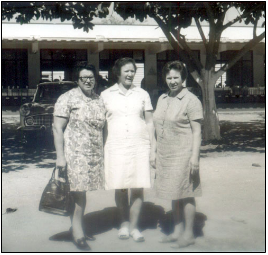
\includegraphics[width = 0.6\linewidth]{9/tias-1.png}
\caption{Tia Imaculada, Tia Glória e Tia Antonieta, num passeio de domingo.}
\end{figure}

Um belo dia, Tio Ângelo quis que elas fossem visitá-lo no Rio.
Ele tinha construído uma enorme casa na praia de Sepetiba como contrapartida à remoção do centro de umbanda da sua mulher para aquele subúrbio e aproveitou para estender o convite a toda a família.
Passaríamos o Natal lá, naquele tempo uma idílica colônia de pescadores, ainda.
Devíamos ir todos, desde o recém-nascido Joãozinho, meu irmão, até Tio Zé e Tia Yolanda, sempre arredios.


O comboio partiu de Araraquara com uma semana de antecedência.
À frente ia a nossa Kombi, porque Papai era um bom conhecedor das estradas, levando nossa família, Tia Imaculada, Tia Glória, Tia Neta e uma parte substancial da merenda, para nossa alegria.
No meio, seguia o caminhão do Tio Totó carregando sacos de frutas, de arroz, de feijão, de milho-verde, engradados de frangos, porcos e cabritos vivos, tudo envolto num inacreditável amarrado de lona que não podia ser muito fechado para não sufocar os animais, mas, ao mesmo tempo, devia ocultar suficientemente a carga para não causar embaraços com a polícia rodoviária, que certamente não acreditaria quando dissessem que tudo aquilo se destinava a mitigar os gastos dos anfitriões com a alimentação daquele bando de glutões.
Desse arranjo resultou que logo no primeiro solavanco da estrada de terra (o asfalto só começava cerca de uma centena de quilômetros antes de São Paulo), parte da lona se desprendeu e para garantir que ela não voasse de vez, assentaram sobre a carga os cento e trinta quilos do Tio Bepe, o que teve a vantagem adicional de desapertar a cabine onde se espremiam Tio Totó e Tia Albina, outra gordinha.
Como Tio Bepe estava ficando careca, amarraram-lhe sobre o cocuruto um lenço à moda dos paisanos da velha Itália, com nós nas quatro pontas para um melhor ajuste anatômico.
E lá seguiu a geringonça, lona enfunada qual uma caravela sobre rodas, ornada no topo pela imensa figura na qual se misturavam em estranha combinação a elegância do terno, de que Tio Bepe jamais abria mão, mais o lenço branco arrematando aquele carão arroxeado pelo maçarico de um sol de dezembro.

Fechando o cortejo, arfando, seguia a ``ximbica'' do Tio Zé, um Fordinho 29 na versão utilitária que um dia, como se depreendia das pequenas manchas visíveis aqui e acolá entre as grandes extensões de tinta de fundo, fora de um belo azul-celeste.
Esta viatura caracterizava-se por ser um primor da criatividade cabocla que o Tio Zé tão bem representava.
A ignição, eu me lembro, era dada por meio de uma chave elétrica dessas montadas numa base de cerâmica, como as que ligavam as máquinas do meu pai, na fábrica.
Era uma adaptação de que Tio Zé se orgulhava por superar em muito, de acordo com ele, a rasteira eficiência das partidas originais de fábrica.
O assoalho, que de há muito apodrecera de ferrugem, fora habilidosamente substituído por tábuas de madeira por cujos vãos se acompanhava a passagem da estrada sob as rodas, vantagem que compensava de sobra os banhos que a tia levava quando atravessavam as poças de água ou lama.
Os faróis também mereceram um importante melhoramento resultante de horas de pesquisa daquele gênio matuto.
Por via das dúvidas, decidiu-se não viajar à noite, porque embora o Tio gabasse a qualidade indiscutível daqueles holofotes adaptados, a verdade é que eles não iluminavam mais do que velas de sebo.
Havia muitas outras intervenções que a minha pouca familiaridade com a mecânica de carros me impedia de alcançar na época, muito embora Tio Zé não se importasse de explicá-las didaticamente a quem se interessasse e até demonstrasse um enorme prazer em fazê-lo.
Mas o mais preocupante de tudo era ele mesmo, o motorista.
Tio Zé tinha inexplicável atração por barrancos.
Tinha o vezo de por nada, assim que divisava lá longe a aproximação de um carro na direção contrária, arremeter para fora do caminho, o que acabou por conferir à pobre “ximbica” aquele aspecto de camuflada.
As consequências só não eram mais catastróficas porque ela rodava muito devagar em virtude de outra criação do Tio Zé destinada a economizar combustível.
Ela quase não gastava, mas também não andava.
Assim, a cada trecho, parávamos no acostamento e rezávamos contritamente por cerca de quarenta minutos até que percebíamos no horizonte aquele pontinho negro movendo-se como cavalo passarinheiro para lá e para cá na estrada.
Aliviados íamos adiante, seguros de que eles ainda nos seguiam.
A todas essas, Tia Yolanda, sentada ao lado do marido, mantinha a dignidade de uma dama inglesa a bordo do seu Rolls-Royce.

É bem verdade que o caminhão do Tio Totó também não era grande coisa.
Meu tio era famoso pela displicência com seus veículos.
Um farol apenas lhe bastava, freio de mão era supérfluo porque ele nunca se lembrava de acioná-lo quando parava num lugar qualquer da sua Boa Esperança.
Estacionar também estava fora de questão.
Quando lhe dava na telha, apeava no meio da rua, como quem desmontasse de um cavalo e nem se dava ao trabalho de fechar a porta, ou retirar as chaves.
O que facilitava para os munícipes a tarefa de deter o carro quando começava a rolar rua abaixo.
Seu genro conta que ele encheu de leitõezinhos vivos para levar para a fazenda, um sedã retirado um dia antes da concessionária, novinho em folha.
Na rodovia que o levava da cidade à fazenda, mal se pilhava numa reta, adormecia.
Acordava-o um cutucão da Tia Albina ou, se ele estivesse sozinho, o solavanco do carro saindo da pista para o acostamento.
Repunha o carro no prumo e voltava a dormir.
Quando íamos com ele para a fazenda, as tias nos instruíam a fazer todo o barulho possível para evitar os cochilos.
Contudo, milagrosamente, Tio Totó só sofreu dois acidentes de monta em toda sua vida: um, quando dormindo, como sempre, errou a ponte e focinhou no rio Jacaré e outro, o acidente que o matou, já nonagenário, quando, ao que tudo indica, enfartou dirigindo.

 
Em Aparecida do Norte, meio da viagem, mais ou menos, fizemos um pouso.
As tias queriam conhecer a basílica da santa milagrosa.
A visita nos tomou a manhã do dia seguinte, de modo que resolvemos almoçar por ali.
O pedido no restaurante foi exagerado, mesmo pelos padrões dos Filpi, e assim sobraram três frangos assados que Tio Bepe mandou embrulhar e que, tão logo reassumiu seu posto sobre a carroceria do caminhão, pôs-se a saborear calmamente, a pretexto de que o tinham apressado demais durante a refeição.
E, por falar em exagero, Pepone parece ter achado excessiva também a gorjeta que meu pai e Tio Totó deixaram sobre a mesa, de modo que, deixando-se ficar por último à saída, tratou de corrigir o despropósito, metendo no bolso dois terços das cédulas.
Quando retornamos à estrada, suponho que intrigado com o aspecto esquisitíssimo da carga mal ajambrada, encimada por aquela paquidérmica criatura de terno atracada aos seus frangos, um guarda fez sinais frenéticos para que o caminhão parasse.
Tio Totó, porém, avançou impavidamente, lona a todo o pano, largando para trás o sujeito espumando de ódio impotente.

Ao fim da viagem, já ao anoitecer, fomos festivamente recebidos pelos tios à porta da casa que mais parecia um pequeno hotel.
Eram catorze quartos cheios de beliches e fartamente abastecidos com ventiladores e bombas de inseticida.
Três horas depois, banhados, jantados e finalmente adormecidos, descobrimos o porquê das medidas preventivas: acordamos sob o ataque do mais formidável exército de pernilongos que eu jamais experimentei em toda minha vida, em qualquer canto desse país.
 Isso em meio a um lago de suor que nos ensopava os pijamas e os lençóis.
Um suplício completo.
Onde estavam os ventiladores, perguntávamos de quarto em quarto, nos debatendo entre as nuvens daquelas minúsculas e sanguinárias feras e o cheiro intenso do veneno espalhado pelo ar.
Tinham misteriosamente desaparecido.
Ninguém conseguia mais ficar na cama.
Apenas um quarto, entre todos, permaneceu fechado: o do Tio Bepe.
Invejosos da insensibilidade daquele bruto que conseguia dormir naquele inferno, passamos o resto da noite a caminhar e a nos abanar até que, pelo amanhecer, decidimos ir deitar na areia da praia.
Na volta, encontramos Tia Neta furibunda: fora arrumar a cama do gordo e, acreditem, ao redor da cama dele ainda funcionavam a plena carga todos os ventiladores desaparecidos! 

\begin{figure}[H]
\centering
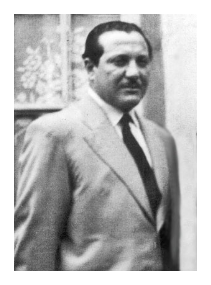
\includegraphics[width = 0.6\linewidth]{9/pepone.png}
\caption{O garboso Pepone, quando jovem.}
\end{figure}

E essa seria só mais uma das muitas gracinhas perpetradas por aquele folgado.
Em dois dias, como acontece desde sempre nas pequenas cidades praieiras do nosso país, o abastecimento de água entrou em colapso.
Tio Ângelo imediatamente contratou um caminhão pipa para encher os reservatórios da casa todas as manhãs.
Para beber, ele trazia engradados de água mineral, à tardinha, quando vinha do Rio.
Contudo, o caminhão pipa, dado o excesso de demanda, não era muito pontual e um dia, voltando da praia, mortos de sede naquele calor, descobrimos que não havia em toda a casa uma única gota de água.
Exceto num lugar, conforme voltou anunciando Tia Neta, que se afastara para investigar o fenômeno, já intuindo a causa: lá fora, num cercadinho improvisado em banheiro, um Tio Bepe feliz da vida acabava de enxaguar seu agora refrescado corpanzil com a última garrafa de água mineral dos dois engradados inteiros que usara para tomar seu banho matinal.
Língua de fora, tivemos que peregrinar de boteco em boteco da vilazinha atrás de água para beber, até que Tio Ângelo chegasse à noite com um novo suprimento.

Nunca entendi porque, mas Tio Bepe, entre os irmãos, gozava de uma inimputabilidade de índio.
Tanto que por muito tempo pensei que ele fosse o mais novo.
Não era.
Aliás, estava entre os mais velhos.
Só não lhe achavam graça Tia Neta, a rebelde, e Tio Zico, esse sim, o caçula dos homens.
Tanto que, num outro dia, deparamo-nos com este último aos berros, apoplético, ameaçando beber o sangue daquele gordo parasita.
Pois ele, Zico, tinha trazido da famosa confeitaria Colombo, a peso de ouro, alguns quilos de uma azeitona espanhola recheada, com a intenção de servi-los aos irmãos como aperitivo para o almoço.
Para tanto, deixara a praia mais cedo, a tempo de certificar-se de que tudo estava preparado e as bebidas devidamente geladas.
Qual não foi sua indignação quando divisou Tio Bepe no terraço, refestelado na espreguiçadeira, ao lado do pote das preciosas azeitonas e cercado de garrafas vazias de cerveja.
Aquele Pantagruel tinha devorado quase todas as azeitonas sozinho e ainda reforçara o ato criminoso com uma verdadeira devastação no estoque de bebida gelada.
Daquela vez, Pepone escapou por pouco de ser lançado por cima da balaustrada.
Livrou-o a chegada dos irmãos que a custo seguraram o mais novo, tomado de ódio assassino.

Uma noite, um pouco antes do fim da temporada, Tia Mariazinha, a anfitriã, brindou-nos com uma sessão no seu recém-inaugurado centro de umbanda.
Exibição magnífica de ritmos e cores.
Lá pelas tantas, as entidades já incorporadas nos seus respectivos cavalos aproximaram-se dos visitantes para dar-lhes o passe de preceito.
Os irmãos Filpi foram enfileirados em ala e o que se seguiu foi para minha mãe a mais inesquecível recordação dessa viagem e a comprovação inequívoca e para sempre lembrada de tudo quanto ela dizia a respeito do gênio selvagem da família do marido: apenas iniciado o ritual, como pedras de um dominó, os caboclos foram caindo para trás duros e tesos, como que fulminados por raio.
Mamãe voou para a porta e foi estourar de riso lá fora, protegida pela escuridão.

\begin{figure}[H]
\centering
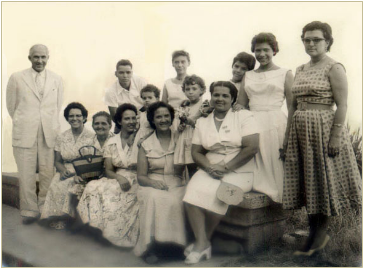
\includegraphics[width = 0.6\linewidth]{9/viagem-a-sepetiba.png}
\caption{Uma lembrança da viagem a Sepetiba: as tias, primos e nossos anfitriões, Tio Ângelo, de pé à esquerda e Tia Mariazinha, sentada à direita, de colar e costume branco.
Na extrema direita, Tia Ilka, a mulher do Tio Zico.}
\end{figure}


Passado o Ano Novo, voltamos para Araraquara e certamente ficou por muito tempo na memória dos caiçaras de Sepetiba a lembrança daqueles alienígenas que lhes consumiram toda a produção de peixe e camarão daqueles dias, pagando nababescamente por isso, bem como a estranha aparição dos tios fazendeiros, madrugadinha ainda, para acompanhar a saída dos barcos, entrando mar adentro de chapelão boiadeiro, camisa de mangas longas abotoada até o pescoço, calção, meias e botinas de elástico.
Todos os dias, enquanto lá estivemos.

As tias conheceram uma das suas poucas férias de Natal.
Porque enquanto puderam reunir os irmãos, era na casa delas que essa festa acontecia.
Da véspera do dia vinte e cinco de dezembro até o dia dois de janeiro, elas se revezavam num absurdo mutirão destinado a manter cheio o prato de no mínimo quatro ou cinco dezenas de pessoas que mal se levantavam da cadeira entre uma refeição e outra.
\chapter{}
As sempre lembradas festas de fim de ano da nossa família alcançaram seu apogeu quando as tias se mudaram para a sua nova casa, na Rua Carlos Gomes, por volta de mil novecentos e cinquenta e cinco ou seis, por aí.
A casa tinha um grande quintal calçado de pedras e uma cozinha nos fundos, equipada com um belo fogão a lenha.
Uma semana antes do Natal, quando os tios do Rio anunciavam sua iminente chegada, sob o comando do tio Bepe, uma grande barraca de lona era erguida no local.
Ao comprido dessa tenda, com tábuas e cavaletes, uma mesa extensa era preparada para receber umas cinquenta pessoas, pelo menos.
Então, tinha início a trabalheira.
Da fazenda, Tio Totó e Tio Zé traziam engradados de frangos, leitoas e cabritos, além de quartos de boi.
Papai se encarregava das bebidas.
Tia Yolanda vinha reforçar a brigada da cozinha aonde a lida ia do amanhecer ao anoitecer, sem parar.
Os animais eram abatidos, limpos, esquartejados e postos em vinha d’alhos.
Panetones, canarícoles, estrufules, bolos de especiarias, compotas, espalhavam seu perfume por todo o quarteirão.
Quilos de massa de trigo eram sovados pelos poderosos braços da Tia Glória, para fazer os pães e o macarrão que seriam consumidos em quantidades industriais.
Grosas de tomate maduro cozinhavam em panelões por horas a fio para fazer o molho do espaguete, do nhoque, dos raviólis, dos fuziles trabalhosamente enrolados um a um, com a ajuda de arame grosso.
Um enorme barril de chope era posto a gelar e era apenas o primeiro dos quatro ou cinco a serem esgotados até o início do novo ano.

Assim que os tios do Rio e respectivas famílias estacionavam à porta, a grande comemoração tinha início.
Meus avós maternos, assim como todos os outros parentes araraquarenses e os parentes dos parentes, noivos, namorados, amigos dos amigos, a partir desse momento tomavam na própria casa apenas o café da manhã.
Para o almoço, seguiam para a casa das tias e de lá só saiam no princípio da madrugada, gratos e empanzinados pela farta, alegre e incansável hospitalidade delas.

Hoje, não vejo como seria possível promover uma comilança daquela envergadura.
Contando, ninguém acredita.
Mas a verdade é que naqueles tempos em que não se discutia triglicérides e colesteróis, aquela gente entregava-se desbragadamente ao prazer de comer sem culpa e esse fato contribuía com parte considerável do sucesso da festa.
As tias percorriam léguas do fogão à mesa e de volta ao fogão, levando travessas cheias e trazendo de volta as vazias para enchê-las novamente.
Frituras crocantes, assados envernizados de gordura, massas nadando em molhos, doces lambuzados de mel, de calda de açúcar, de cremes, nada intimidava os animados convivas sempre capitaneados pelo Pepone cujo perfil, lá pelas tantas, começava estranhamente a assumir o contorno do barril de chope que ele cuidava de esvaziar em grandes e entusiasmados sorvos, dignos de um guerreiro viking.


Por volta da meia-noite da véspera do Natal, as tias desapareciam momentaneamente do cenário, não sem antes abastecer a mesa mais uma vez, para que ninguém ficasse desassistido enquanto elas corriam até a Matriz para a Missa do Galo.
Raras vezes alguém deu pela falta delas.


Início da madrugada, Pepone, já liberto de todas as amarras, dava início aos discursos e aos brindes.
Aos \textit{hip}, \textit{hip}, \textit{hurras!} e vira-viras que acompanhavam a competente ingestão de mais alguns canecos de chope, todos os presentes recebiam vivos agradecimentos pela honrosa presença e eram postos a par da tradição de hospitalidade que distinguia os Filpi desde Novi Veglia, na distante Salerno, até o momento em curso.
Nessa nostálgica trajetória, Tio Bepe, flutuando nos vapores do chope, ia se emocionando progressivamente até chegar à lembrança da ``nossa santa mãe'', referência que sempre fazia chegar lágrimas aos olhos de todos os machos da família, orador incluído.
Apenas meu pai se continha, consciente da expressão zombeteira que assomava ao rosto da minha mãe, sempre que os cunhados se punham a canonizar ``aquela virago''.
Nesta altura, Tio Totó intervinha e tomava a palavra, coisa que ele perceptivelmente desejava fazer desde o início, afinal o político ali era ele, e completava a elegia com merecidas homenagens ``às nossas santas {\large\bfseries ermãs}'', como ele dizia.
Mais alguns \textit{hip-hurras}, aplausos e Tio Bepe, já recuperado do surto emocional, mas não da bebedeira, bradava seu grito carnavalesco predileto -- \textit{“Alalaô, ooô, ooô! Mas que calor, ooô,ooô!”}, -- e arrastando todo mundo para o cordão de que ele assumia o comando logístico–musical, punha-se a evoluir pela casa até cair semi-desmaiado em algum canto.
Houve um ano em que se superando, ele concluiu sua performance exibindo-se num sapateado de elefante amestrado sobre o barril vazio, para assombro dos circunstantes.


\begin{figure}[H]
\centering
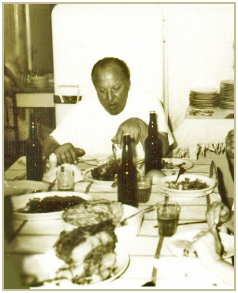
\includegraphics[width = 0.6\linewidth]{10/pepone-natal.png}
\caption{Pepone presidindo a mesa de Natal.}
\end{figure}

Ano após ano, ainda que soubéssemos que o enredo era sempre o mesmo, por nada perdíamos as festas de fim de ano na casa das tias.
Enquanto as quatro juntas puderam agüentar aquela verdadeira maratona culinária com a mesma disposição e a mesma generosa alegria, ninguém ali pensou em desfrutar o final do ano em outro lugar.

Quando Tia Glória, a última das irmãs a ir-se deste mundo, estava próxima da morte, eu a visitava diariamente.
A tia já há anos vivia imobilizada na sua poltrona, mas continuava lúcida e, nesse final de vida, tornara-se sábia, não obstante ter passado a maior parte dos seus oitenta e dois anos à beira de um fogão.
Numa tarde telefonou-me, pedindo que especialmente naquele dia não deixasse de ir vê-la, pois tinha um pedido a fazer.
Fui.
A tia estendeu-me um caderno onde estavam anotadas as receitas que por dezenas de anos tinham feito a fama da sua cozinha.
Queria que eu a ajudasse a selecionar aquelas mais fáceis e saborosas para reuni-las num livrinho que pudesse enviar às sobrinhas do Rio.
\textit{``-- Você pode fazer isso bem organizadinho no seu computador, não pode?''}, quis saber ela.

Disse que podia.
Então, ela justificou o pedido mais ou menos assim:
\textit{``-- Filha, você e suas primas daqui conviveram conosco, aprenderam a cozinhar direitinho e sabem da importância de reunir a família em torno de uma mesa, partilhando uma comida bem feita, gostosa.
Foi assim que mantivemos nossa gente unida por tanto tempo.
Tem quem possa achar que eu fui infeliz, dedicando a minha vida toda a cozinhar para vocês.
Mas hoje, olhando para trás, penso que essa foi uma missão que me destinaram e sou feliz por tê-la cumprido direito.
Fico preocupada com essas sobrinhas lá longe, vivendo numa cidade tão grande e tão difícil.
Sabe-se lá se têm tempo de preparar alguma coisa para os maridos e os filhos.
Essas receitas elas poderão fazer em poucos minutos, sem perigo de errar.
Todas foram testadas muitas vezes por mim.
Assim morro sossegada, sabendo que elas também poderão reunir sua gente em volta da mesa, como sempre foi na nossa família.
Você pode mandar junto com o livrinho uma carta, explicando isso tudo?''}

\begin{figure}[H]
\centering
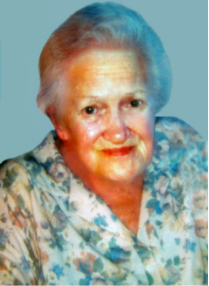
\includegraphics[width = 0.6\linewidth]{10/tia-glória.png}
\caption{Tia Glória aos 81 anos.}
\end{figure}

E foi dessa maneira que, naquela tarde, ajudei Tia Glória a lavrar o que, me parece, foi seu único testamento, ou, melhor dizendo, sua confissão de fé.
 

\chapter{}
Quando morávamos junto da Fábrica do meu pai, no quarteirão defronte, num canto do terreno ocupado pelo almoxarifado da Prefeitura, instalavam-se os parques de diversão e circos mambembes que passavam pela cidade.
Num tempo em que ainda não se ouvia falar de \textit{playcenters}, \textit{playgrounds} e \textit{videogames}, a chegada de um deles punha a meninada em completo alvoroço.
Se era um circo, acompanhávamos dia após dia o descarregar dos caminhões, ansiosos para saber se era do tipo que trazia tigres, leões e elefantes, ou, mais empolgante ainda, o globo da morte com seus intrépidos motociclistas e suas máquinas barulhentas.
Na maior parte das vezes, porém, o que aparecia eram os chamados circos-teatro, quase indigentes, em que o ralo elenco, dono incluído, revezava-se nos malabares, no trapézio, na bilheteria e, ao grande final, subia ao palco para encenar o ponto alto do espetáculo, o drama em três atos sempre farto em suspense, lágrimas e punhaladas que encerrava a noite.
Mais divertido para nós, era descobrir, sob a pesada maquilagem, o palhaço agora travestido de pai cruel da infeliz mocinha em quem reconhecíamos a bailarina da corda bamba, chorando copiosamente de amor contrariado pelo galã, que pouco antes víramos a dar saltos mortais, pendurado às barras do trapézio.

Nesses circos-teatro em que o magro programa arrastava-se em perfeita consonância com a penúria do empresário e dos artistas, organizavam-se, nos intervalos entre um número e outro, concursos de cantores, de lutadores, de dançarinos, recurso infalível para acender a imaginação dos candidatos a celebridade e salvar a bilheteria do dia.


Uma vez, tinha eu sete ou oito anos, sabe-se lá por que, em absoluto segredo, inscrevi-me para cantar num desses concursos.
Eu fazia parte do orfeão da escola e era elogiada pela minha afinação.
O concurso seria na matinê de domingo.
Aproveitando que meus pais sempre tiravam uma soneca após o almoço desse dia, saí despercebida de casa, encarei a batalha de vencer a timidez e a pouca confiança na minha aparência mais do que rechonchuda e me apresentei ao organizador do concurso, na coxia.
Ao seu sinal, subi ao palco e assim que anunciado meu nome, comecei a cantar um bolero, imaginem só.
Foi aí que lá de cima, olhando aquele monte de desconhecidos me fitando, dei-me conta do ridículo e do descabido da situação.
Vacilei e pior, nesse momento o palhaço aproximou do meu rosto o seu carão brilhante de suor e alvaiade e, no susto, minha voz foi sumindo num fio e desapareceu por completo.
E eu nem sabia que nessa altura meus pais, alertados pelo som do meu nome no alto-falante, tinham acordado e, estupefatos, procuravam entender como sua tímida e roliça pata-choca decidira tentar o estrelato.
Saí debaixo de vaias e aplausos de consolação.
Se bem me lembro, papai e mamãe tiveram a gentileza de não aprofundar o assunto diante do meu furioso silêncio.
Já o mano e seus amiguinhos da rua não deixaram passar a oportunidade, fazendo do meu vexame a manchete da semana.
Agüentei calada.
Achei que merecia.
 Contudo, eu logo teria uma meia vingança.


Quando pouco depois nos mudamos para a casa nova, do outro lado da cidade, coincidentemente estendia-se diante dela um imenso terreno baldio, também de propriedade da Prefeitura e para o qual, a partir dessa época, seria transferida a montagem de parques e circos de passagem pela cidade.
Um dia, um vizinho, rindo, veio chamar meu pai para espiar seu promissor rebento, Reginaldo, de tabuleiro pendurado ao pescoço, vendendo amendoim torrado nas arquibancadas.
Meu irmão tinha arrumado o negócio com o pipoqueiro, em troca de entrar todo dia no circo, de graça.
Por pouco, não tomou uma coça.
Foi poupado pelo espírito de iniciativa que revelou, o que, no meu caso, ninguém levou em consideração.
Bem, pelo menos não tomei pito como ele.

O que eu gostava mesmo era dos parques de diversão com seus carrinhos coloridos, a roda gigante, as barracas de tiro ao alvo, de jogo de argolas, de pescaria, que me faziam sonhar com a boneca de vestido rodado ou o urso de pelúcia oferecidos como prêmio.

Eu não me arriscava nos brinquedos que giravam vertiginosamente provocando náusea, ou ameaçavam precipitar a gente no vazio.
Nunca compreendi onde está a graça de associar diversão à tortura.
O brinquedo de que mais gostava eram uns barquinhos, dentro dos quais, puxando uma corda passada em torno de uma roldana suspensa, a gente conseguia balançar cada vez mais forte, cada vez mais alto, dependendo só da força dos nossos braços.
Pelo preço do ingresso, o dono do brinquedo nos deixava ficar lá por uns quinze minutos, o que sempre me parecia pouco demais.
Bom mesmo era quando o sujeito se engraçava por uma daquelas mocinhas que flanavam por ali e, empenhado na conquista, esquecia-se do tempo.
Os minutos de lambuja que ganhávamos dessa maneira pareciam os melhores.
Um olho na corda, outro no namoro, eu tratava de ir cada vez mais alto e o medo de que o homem acordasse para o prejuízo e empurrasse para baixo do meu barco aquele calço de borracha que decretava o fim da brincadeira, chegava a dar um frio na barriga, de tanta tensão.

Muitas vezes, quando penso na Morte, o que me vem inevitavelmente à lembrança, como irresistível analogia, é aquele momento de agônica ansiedade durante o qual eu espreitava o tal sujeito, temendo ver seu olhar indiferente voltar-se na minha direção e, sem nem se importar com minha expressão de súplica, meter por baixo do meu barquinho aquele naco de pneu que, por mais que eu puxasse a corda com todas as minhas forças, ia inexoravelmente segurando-o, segurando-o, até detê-lo por completo.
Ah, se ela se distraísse por um instante e me deixasse brincar só um pouquinho mais\dots
\chapter{}

\begin{figure}
\centering
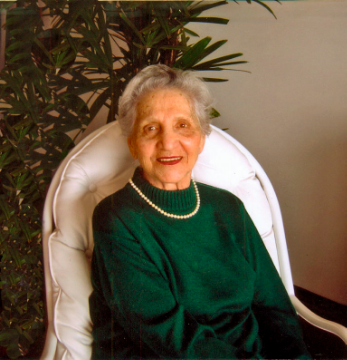
\includegraphics[width=0.6\linewidth]{12/odila.png}
\caption{Tia Odila.}
\end{figure}

Quem conheceu Tia Odila, a irmã mais velha da mamãe, acha que eu me pareço mais com ela do que sua própria filha, Maria Sílvia.
Talvez porque como eu, Tia Odila sempre tenha sido uma mulher grande e forte, obesa até, durante os anos mais difíceis da vida dela.
O corpo generoso, mas bem feito, combinado a uma postura ereta e altaneira comunicava tal impressão de autoridade que ela parecia maior do que de fato era.
Uma gorda elegante.
Mesmo nos seus últimos dias, debilitada pelos sucessivos colapsos do coração, recostada numa poltrona para que o ar não lhe faltasse, esforçou-se por manter a cabeça erguida durante nossa breve conversa e o roupão que envolvia seu corpo definhado ainda era envergado como se fosse arminho.
Ai de mim, essa pose um tanto imperial que a caracterizava, mais de uma vez foi apontada como outro dos traços que nos faziam parecidas.
Mesmo Paulo manifestou muitas vezes o temor de que a semelhança fosse muito além da mera aparência.
Mas, embora admitindo que, como acontecia com ela, muitas vezes minha postura sugeriu às pessoas certo autoritarismo, a identificação nunca existiu além da superfície.
Porque, no meu caso, a atitude servia apenas à causa de vencer a timidez e disfarçar o andar inseguro, mas, no caso dela, havia uma história a justificá-la.

Como Tia Yolanda, Tia Odila foi originalmente educada para voos mais altos do que o árduo e mesquinho caminhar que a vida lhe impôs.
Cedo demonstrou talento para o piano e chegou mesmo a sonhar com uma carreira de concertista, depois que, levada à presença da afamada pianista Antonieta Rudge, ouviu desta os mais calorosos incentivos.
Os estudos lhe custaram sacrifício e paciência porque pianos eram caros e só muito tempo depois de praticar em instrumentos alheios, Tia Odila conquistou o seu.
Já então começara a dar aulas de música para ajudar em casa.
Havia o curso de normalista a pagar no Colégio Mackenzie, pois a Vovó fazia das tripas coração, mas as filhas tinham que estudar em escola particular, na companhia dos rebentos das melhores famílias da cidade.
E havia as duas irmãs menores para vestir e calçar.
Tia Maria Angelina, a caçula, sempre mencionou com gratidão os vestidos e sapatos que a Tia Odila lhe comprava nas melhores casas da cidade, pagando com os magros rendimentos da sua dupla jornada de professora primária e professora de piano.
Já minha mãe não teve essa sorte.
Porque mamãe cresceu em meio à penúria que se seguiu à falência da Mobiliadora que Vovô assumira após a morte do cunhado e, à crise de 1929, que agravou ainda mais a situação da família, jogando o coitado na vala dos desempregados por longos anos.
Durante esse tempo, foi Tia Odila quem assumiu a tarefa de sustentar a casa, secundada pela Vó Didi que dizia rindo, mais tarde, que nesses dias amargos fez de tudo, só não “fez a vida”, eufemismo que ela usava para designar a atividade do meretrício.
Vovó Didi, todos conhecemos a história, fez sabão, linguiça e pão para vender, deu pensão, costurou para fora, mas nunca sobrava para os vestidos novos com que minha mãe sonhava e muito menos para levar adiante a naufragada carreira de concertista da Tia Odila.
Até o piano teve que ser vendido.

Uma esperança surgiu quando se enrabichou por Odila o belo filho do Coronel Juca Custódio, um dos poderosos da cidade, dono de muitas terras de café.
Cornélio, assim se chamava o jovem herdeiro, era bonito, mulherengo e estroina.
Passava os dias no clube, jogando cartas e as noites nos cabarés da cidade.
Tia Odila tomou a peito, como era bem próprio dela, a tarefa de fazer dele um homem.
Com apoio integral da sogra, Dona Cornélia, lançou-se à missão antes mesmo de subir ao altar.
Mas a empreitada seria muito mais longa e difícil do que supunha.
Sucessivos e variados negócios foram montados antes e depois do casamento na tentativa de conseguir que Tio Cornélio se tornasse um adulto responsável.
Sem sucesso.
Por variadas e sempre muito bem explicadas razões, os empreendimentos não prosperavam.
E tia Odila era quem mais caprichava na defesa do companheiro.
Era mesmo falta de sorte ou conspiração de despeitados.
Nunca alguém ouviu dela, pela vida inteira, qualquer palavra que desabonasse o marido, por mais que os fatos falassem por si.
Tia Odila aprendeu a engolir as decepções e a erguer o queixo voluntarioso na direção inversamente proporcional à frustração que lhe descia goela abaixo.
Dona Cornélia, a sogra, uma aristocrática senhora que eu conheci e que muito me impressionou com seu perfil de camafeu realçado pelo fichú de rendas e coroado por alvos cachos, ensinou-a a cultivar maneiras de uma grande dama.
As bonitas mãos de pianista resumiram toda a sua vaidade e foram sempre cuidadas com devoção e orgulho.
Embora na maior parte do tempo não pudesse contar com o luxo de uma empregada, Tia Odila era capaz realizar todo o trabalho doméstico com maestria, sem riscar sequer o esmalte das unhas impecavelmente manicuradas.
Como professora, foi igualmente competente.
Organizada ao extremo, caminhava pela casa e pela sala de aula com a serenidade e a segurança de quem portasse uma varinha de condão.
E tudo que saía das suas mãos era perfeito.


Tia Odila foi mais um dos meus modelos de ser humano.
Sob muitos aspectos não me identifiquei com suas posições de vida e até discordei, e muito, de algumas delas.
No entanto, aprendi a admirá-la pelo que ela teve de herdeira legítima da garra e da força das mulheres Credidio.
Na defesa dos seus era capaz de ir a extremos de esforço e sacrifício.
Se pecou, foi por excesso.
Os jesuítas ensinam que o mal das árvores que projetam muita sombra é que sob elas nenhuma outra planta prospera.
Com Tia Odila aconteceu assim.
Guerreira e determinada, tomou para si, desde cedo, a missão de lutar pela felicidade dos que a cercavam, marido, filhos, parentes, doentes, carentes, quem quer que ela decidisse necessitar de ajuda.
Por cima de paus e pedras, a favor da corrente ou contra, se preciso fosse.
Mas acabou aprendendo que a Vida é sempre maior, quando esta lhe impôs algumas e severas derrotas.

No que toca ao tio Cornélio demorou, mas tia Odila venceu.
Ele acabou por se tornar, afinal, um chefe de família exemplar.
Um dominado pela mulher, opinava a maioria dos parentes.
Pessoalmente, discordo.
Era um menino que nunca amadureceu.
Tia Odila proporcionou-lhe dignidade e o carinho e o respeito dos filhos.
Nomeado tesoureiro da companhia de transportes urbanos de São Paulo, a CMTC, por empenho da mulher, rendeu-se finalmente ao trabalho que realizou honesta e pontualmente até aposentar-se, orgulhoso, aliás, da sua grande responsabilidade.
Vinha almoçar trazendo algemada ao pulso uma pasta que tia Odila solenemente retirava e punha em segurança.
À nossa imaginação de crianças, isso sugeria encargos misteriosos e secretos, impressão que Zé Vicente, seu filho e nosso primo, tratava de reforçar esclarecendo que as algemas eram necessárias porque o conteúdo da tal pasta era tão importante que deveria ser defendido até mesmo com a própria vida pelo pai.
Diante dos nossos olhos arregalados, Tio Cornélio sorria envaidecido.


Por toda sua existência, fora do trabalho, o tio acomodou-se à situação de deixar-se cuidar e orientar docilmente pela companheira.
Ela o chamava de “Menino Jesus” e vigiava-lhe minuciosamente os atos e os passos.
O que bebia, comia, vestia e fazia.
E ele se submetia.
Foram felizes assim.
Os machos da família torciam o nariz.
Mas não sei se, sozinho, algum dia ele se tornaria alguém.
Será?

Como mãe, tia Odila manteve-se fielmente atrelada à convicção de sempre saber o que era melhor para os filhos e, baseada nisso, a tomar decisões por eles.
Nunca pude concordar com essa postura, embora até a entendesse.
A frustração de não ter conseguido realizar os sonhos que alimentara para si, sublimou-a através de um projeto sólido de alçar Maria Sílvia e José Vicente aos patamares mais altos que pudessem alcançar.
Ela o faria por eles, como uma dádiva.

Silvinha, como a chamávamos, foi linda desde menina.
Moça, fez-se alta, magra, dona de grandes olhos ambarinos e de um porte de princesa.
Ah, Tia Odila queria seu futuro nas colunas sociais, com direito a tudo que a sua beleza fazia por merecer, a começar por um casamento cinematográfico, com um noivo lindo, educado e rico.


Tia Odila era muito engraçada e a peça de resistência das suas performances cômicas era o relato do seu próprio casamento, espinho cravado na memória da sua mocidade.
Ouvi-a contá-lo inúmeras vezes e ri até as lágrimas em todas.
Além de terem que se casar às seis e meia da manhã por causa do horário do trem em que partiriam para a lua de mel, fato que levou Tio Cornélio, na hora das alianças, a apresentar ao padre, por engano, a escova de dentes que apressadamente enfiara no bolso, havia a história do vestido e da festa.
O vestido, dada a penúria dos pais da noiva, fora presente da Tia Angelina, modista afamada.
Mamãe sustentava que não por sovinice, mas porque era moda então, o vestido tinha uma cauda tão mínima que, dizia Tia Odila, metia-se-lhe por entre as pernas enquanto ela caminhava em direção ao altar.
Para aumentar-lhe a agonia, dos pés lhe subia ao nariz o cheiro de óleo de banana, base da tinta de purpurina que Tia Lúcia, irmã da Vó Didi e dona da funerária da cidade, usava para enfeitar seus caixões de defunto e que, providencialmente, serviu para transformar um par de sapatos usados nos argênteos sapatinhos da noiva.
Para arrematar o arranjo todo, à guisa de tiara e fazendo as vezes de buquê, flores de sabugueiro, garantia Tia Odila.

{\itshape -- ``Mentira, sua exagerada! Eram botões de laranjeira''}, rebatia minha mãe.

Após a cerimônia, a recepção aos convidados restringiu-se a um modesto e apressado café da manhã, porque o trem não esperava.
Tia Odila jamais se conformou.
Bradava, raiando a fúria, que com a filha não seria assim.
Silvinha se casaria com tiara de estrasses e, quando chegasse ao altar, a cauda e o véu ainda se arrastariam à entrada da igreja, haviam de ver, nem que ela tivesse que deixar de comer para realizar esse sonho.
E a festa seria de arromba.
Com bufê e garçons, para toda a família.
Fazia questão.

E assim, foi.
Silvinha se casou com um jovem bonito, educado e rico.
Levando um enxoval de rainha que custou à tia Odila dois anos de economia insana.
Foi a única vez nesse mundo em que alguém a viu usando meias de seda remendadas.
Mas, chegado o dia, Silvinha pisou o tapete vermelho como que saída de um conto de fadas.
Magnífica.
Arrastando uma cauda enorme e ostentando, sobre a cabeça, uma minúscula coroa a segurar o longo véu.
Nas mãos, orquídeas.


No altar, uma mãe realizada.
E vingada, como confessaria logo depois, olhos ainda marejados de emoção.

O sonho, porém, não durou.
Muito de acordo com a tradição das Credidio, o marido, um príncipe, como gostava de dizer Tia Odila, revelou-se um fraco, um clássico caso de filho único criado com todo o mimo e totalmente despreparado para a vida.
Morto o pai que o orientava e acudia, os negócios foram por água abaixo, levando de cambulhada os bens da mãe viúva e dos sogros que haviam avalizado muitos dos títulos jamais resgatados.
Mãe de três filhos ainda pequenos, minha prima teve que trabalhar duro e como brava representante da estirpe, fez um pouco de tudo: vendeu jóias, cosméticos e roupas, de porta em porta.
Até manifestar os primeiros sinais de Alzheimer, ao  aproximar-se  dos setenta e tantos anos, não encontrou descanso.
Tia Odila teve que vender o apartamento que adorava e mudar-se para um pequenino, que ela odiou até morrer.
Mas nunca deixou de ajudar a filha e ainda teve a satisfação de contribuir para vê-la instalada, ela sim, num bom apartamento para cuja decoração a mãe concorreu com tudo que lhe sobrara de mais precioso.

Já o filho, José Vicente, esse foi desde menino a grande fonte das suas preocupações.
Todos nós o achávamos perfeitamente normal, boa praça, e muito divertido.
Estava longe, é verdade, de devotar-se aos estudos com o afinco que Tia Odila imaginava necessário para torná-lo um doutor como os Ópice, esse era o outro grande sonho dela.
 Contudo, não havia quem resistisse à bondade, simpatia e vivacidade do garoto.
Aos doze anos começou a crescer aceleradamente.
Aos quinze, passara de um metro e noventa.
 Quando parou de crescer, finalmente, alcançara dois metros e seis centímetros.
Tia Odila fez daquilo um drama.
José Vicente era tratado como se feito de porcelana.
Ninguém na família se esquece dela caminhando diariamente até o quartel onde ele prestou o serviço militar, levando uma maleta cheia de comida para o maxi-recruta, temerosa de que reduzido apenas ao rancho, ficasse anêmico.
De quebra, ia lá dentro também o fortificante.
Quando Zezo, era esse seu apelido, passava férias conosco em Araraquara, ela e Tio Cornélio telefonavam todos os dias para saber se ele tinha tomado banho, se tinha limpado as orelhas, se estava calçado e agasalhado.
A todas essas, minha mãe respondia afirmativamente, muito séria, contemplando ao longe um José Vicente imundo, suado de correr atrás da bola num calor saariano, no campinho de terra que havia em frente da nossa casa.


Pois José Vicente tornou-se homem, driblando com carinho e bom humor as investidas da mãe sobre o seu destino.
Não chegou a doutor.
Contentou-se em ser contador, para desgosto dela.
Tentou adotar a política do pai.
Foi trabalhar na Companhia de Energia Elétrica do Estado de São Paulo, como escriturário, e em casa dizia amém, sem contestar.
Mas, um belo dia, não aguentou mais.
Fugiu.
Com sua futura mulher.
Uma colega de trabalho, moça muito simples, bem mais velha e, pior, nem um pouco bonita.
Tia Odila quase enlouqueceu.
Durante uma semana, procurou-se esse rapaz por todos os cantos.
Até uma cartomante foi convocada.
Quando foi encontrado, já era tarde.
Estava casado.
De papel passado.
Não havia para Tia Odila o que fazer a não ser engolir, mais uma vez.
 O diabo é que a tia tentou, mas tenho certeza de que a coisa nunca lhe passou pela garganta.
A situação como um todo e, mais especificamente, a nora.
O filho não se tornara doutor e a segunda oportunidade de chegar a algum lugar, através de casamento vantajoso, também lá se fora, desperdiçada.
Mais do que simples, Teresa, a esposa, era simplória.

Diga-se, a bem da verdade, que todos nós ficamos um pouco decepcionados com a escolha do Zezo.
Ele se tornara um belo homem, com toda aquela altura, encorpado, sorriso cativante.
Por que Teresa?
 
Foi fácil encontrar a resposta, apenas a conhecemos melhor.
Para ela, José Vicente era, é e será sempre o mais talentoso, o mais competente, o mais brilhante indivíduo deste lado do planeta.
Não vê outro que lhe chegue aos pés.
Repete como um mantra que não sabe por que ele nunca se candidatou a deputado.
Também merecem sua admiração os filhos, os amigos e os parentes que tiveram a gentileza de acolhê-la.
Tem uma capacidade genuína e inigualável de empolgar-se com tudo que passa pelo seu campo de visão.
Dizem que quando um casal se diverte junto, encontrou a chave da felicidade eterna.
Pois José Vicente ri o tempo todo com a mulher.


Tendo Teresa por companheira, José Vicente finalmente concluiu os estudos superiores que Tia Odila fez questão de custear.
Formou-se em Administração de Empresas.
Foi, conforme ouvimos de hóspedes que o conheceram, um eficiente administrador dos hotéis da CESP instalados em Jupiá e Ilha Solteira.
Aposentou-se, como o pai, em condições de proporcionar uma vida confortável e sem sobressaltos à esposa, deixando uma excelente impressão seja na lembrança dos superiores, seja na dos subordinados.

Presenciei, não faz muito tempo, toda a família do meu primo reunida.
São três filhos, hoje moços e casados e, como educadora, não pude deixar de admirar a maneira bonita como se relacionam entre si e com os pais.
Três vidas, três trajetórias totalmente diferentes, sortes diferentes e nenhuma inveja, nenhum traço de ciúme ou rivalidade.
Afeto legítimo, alegria autêntica e uma absoluta solidariedade mútua.

Acho e espero que, no fim da vida, tenha se dissipado a bruma do preconceito que por tantos anos impediu minha tia de ver seu filho como realmente ele era e de desfrutar a companhia dessa nora e desses netos sem ressentimentos, de alma lavada e feliz.
Acredito que isso aconteceu, porque foi esse filho quem mais cuidou dela nos seus últimos dias, trazendo-a para a casa dele inclusive, muitas vezes.

 
Quando todos estes revezes aconteceram à minha tia, eu já estudava e morava em São Paulo.
Fui testemunha das suas misérias e da sua grandeza.
Durante a prolongada crise que se instalou com a falência do Artur, marido da Maria Sílvia, toda quarta-feira, se não me falha a memória, ela empreendia uma penosa jornada de ônibus até a Lapa, onde eles moravam, carregando duas sacolas pesadas de verduras, frutas e mantimentos para abastecer-lhes a despensa vazia.
Algumas vezes eu a acompanhei, para ajudá-la.
Tia Odila fez isso durante muito tempo, para que nada faltasse aos netos.
Foram-se as jóias, foi-se o apartamento comprado com as economias de toda uma vida, o da Alameda Franca, com a larga varanda dos fundos e sala com vista para um bonito jardim em terraços.
Sobrou-lhe um quarto-e-sala na Rua Frei Caneca, sobre uma padaria, através de cuja janela, já inválida, ela olhava melancolicamente o prédio da frente.
Porém dela, ninguém ouviu uma queixa.
Nem as irmãs.
Quem a conhecia, percebia que havia dias em que o queixo se levantava mais alto e os lábios se cerravam com mais força.
E era só.
 

Pelo muito que errou e pelo outro tanto que acertou, Tia Odila foi uma grande lição.
Se a Deus agrada aquele que toma a vida nas mãos, vencendo os obstáculos por um esforço de superação aguerrido e contínuo, sem acovardar-se nunca, ela há de estar lá em cima num bom lugar.
Ao qual ela fez jus, principalmente, pelo excedente considerável de boas ações, das caridades que fez motivada por um espírito que me é particularmente caro porque a cada dia vai se fazendo mais e mais raro e que, a meu ver, ombreava-a com a gente do meu pai: o espírito do acolhimento ao outro, da hospitalidade generosa.
A casa da tia Odila, como a das tias Filpi, era uma casa para onde sempre se podia ir, porque ela sempre estava lá, de porta e braços abertos para você, não importa se ela o aprovasse ou não como ser humano.
Se a procurasse, não ficaria sem acolhimento.
E seria tratado como um rei.


Um dia, ela me ensinou: 
{\itshape``-- Quando se mudar para um lugar novo, procure saber e guardar o nome de todos: do leiteiro, do padeiro, do açougueiro, dos vizinhos; chame-os todos pelo nome, dos humildes aos poderosos; trate-os com gentileza; dê mostras todo o tempo de que os reconhece, um a um.
Verá como tudo ficará muito mais fácil.''}

\chapter{}

\begin{figure}
\centering
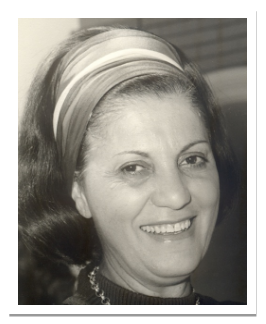
\includegraphics[width=0.7\linewidth]{13/mamãe.png}
\caption{Mamãe, por volta dos cinquenta anos.}
\end{figure}

Minha mãe tinha ideias muito claras sobre o que deveria ser uma preparação eficiente para uma vida de mulher bem sucedida.
Aprendidas ao longo da sua experiência de menina pobre e prudentemente ajustadas aos valores predominantes em nosso meio.
O modelo se desenhava a partir de três orientações básicas: ter ótima aparência, ser uma impecável dona-de-casa e estudar o suficiente para garantir desembaraço social e uma pequena, mas honrosa margem de independência financeira.
O bastante ``para os alfinetes'', para usar uma expressão de época.
O objetivo final do programa, como não podia deixar de ser, era chegar a um casamento assentado sobre uma desejável e sólida base material e afetiva.
Nessa ordem.
A novidade, em relação a tempos anteriores, é que as mulheres do pós-guerra começavam a ter ambições de um tratamento mais igualitário face aos homens.
Tomando cuidado, porém, para não perder as vantagens inerentes à decantada fragilidade do sexo.
Assim, ensinou-me ela que nascer bonita não era essencial, mesmo porque nem todas têm essa sorte, mas, com jeito, simpatia e bom gosto, pode-se parecer bonita e isso, afinal, é o que importa.
Dominar as competências domésticas era imprescindível, mas apenas para saber orientar e governar as empregadas, pois, mesmo sendo de origem humilde, minha mãe acompanhava a crença generalizada de que o trabalho doméstico era degradante.
Embora Hollywood divulgasse a visão encantadora da dona de casa de aventalzinho, feliz na sua cozinha planejada, entre seus eletrodomésticos de última geração, as brasileiras preferiam agradecer a Deus a felicidade de terem nascido numa terra onde não havia nada disso, mas a criadagem era farta e barata.
Quanto a adquirir uma profissão, o aconselhável era escolher uma atividade ``mais feminina'' como o magistério, por exemplo, que pela afinidade evidente com os deveres de uma mãe de família, preenchia o quesito de prover a mulher de um dinheirinho extra para os seus supérfluos, sem comprometer o cumprimento das suas obrigações prioritárias com o lar, o marido e os filhos.
O esforço intelectual exagerado também não era recomendável.
Mamãe dizia que homem nenhum quer mulher metida a sabichona.
Concedia-se, a título de consolo, que as muito feias ou desajustadas que não conseguissem casar, buscassem com mais afinco realizar-se numa profissão.
Mas, se ousassem se destacar além da conta, sobretudo nos estudos, passariam fatalmente à condição de ``esquisitas''.
Muita leitura, muito estudo acabam amolecendo os miolos, era outro dos axiomas que mamãe assimilara do ambiente e gostava de recitar.

Ocorreu, porém, no meu caso, que os belos planos da minha mãe foram frustrados por dois fatores: dos nove aos dezoito anos eu não consegui permanecer magra por mais do que uns poucos meses, o que reduziu em muito minhas possibilidades no mercado casamenteiro e, a partir de certo momento, eu decidi eleger Tia Maria Angelina, a irmã caçula dela, em meu modelo predileto de desenvolvimento pessoal.


Olhando minha adolescência em retrospectiva, é possível entender de que maneira esses fatores se interligaram de modo a formar uma barreira muito sólida atrás da qual me pus a salvo de um destino que inconscientemente eu rejeitava.
Tia Maria Angelina parecia aos meus olhos de menina o suprassumo da modernidade: era bonita, alta, de uma elegância sóbria, casual, personalíssima.
Tocava violão, cantava, tinha um monte de amigos e amigas e parecia levar uma vida bem mais divertida que a das outras mulheres que eu conhecia.
Vez ou outra me levava com ela no seu \textit{Studebaker} azul, outra ousadia, um carrão que ela guiava desafiadoramente pela cidade.
E, incrível, sua irresistível vocação para sacudir aquele mundinho provinciano levou-a a abandonar um noivo praticamente ao pé do altar, ato justificado perante toda a família com o mais cândido argumento:
{\itshape``-- Perdão, mas eu não consigo me ver como dona-de-casa pelo resto dos meus dias, fazendo comidinha, cuidando do maridinho e dos filhinhos.
Sinto muito!''}

Eu não podia avaliar, então, o tamanho da comoção causada por esse gesto.
Mas, acho que de algum modo ela compreendeu que encerrara suas possibilidades de permanecer na cidade.
Em pouco tempo mudou-se para São Paulo, levando com ela Vô João e Vó Didi.

\begin{figure}
\centering
\includegraphics[width=0.7\linewidth]{13/manina+lygia+glória.png}
\caption{Manina e suas amigas, Lygia e Góia (Maria da Glória).}
\end{figure}

Eu resistia o quanto podia ao projeto que mamãe reservara para o meu futuro.
Tive que estudar piano com um professor que eu odiava tanto quanto ao instrumento.
Acho que se me fosse dado escolher, preferia dançar a tocar.
Mas não fui consultada.
Minha primeira apresentação em público foi um fiasco.
Esqueci a música tão longamente ensaiada.


Minha obesidade e minhas pernas tortas receberam um tratamento que incluía ginástica, natação, regimes sucessivos com sucessivos médicos e uns malditos sapatos ortopédicos que, além de divertir muito meu irmão, só resultaram em duas torturantes unhas encravadas e um andar de quem tinha urgência de ir ao banheiro.
Definitivamente, eu estava longe de ser a beldade que a minha mãe sonhava fazer debutar no Clube Araraquarense.

Ah, e havia o nariz: eu herdara do meu pai um nariz de batata que no rosto dele reforçava certa rusticidade máscula, mas em mim, eu sabia, exercia um efeito devastador.
Mesmo que Tia Maria Angelina me assegurasse que meus olhos e minha boca eram lindos, eu não me convencia de que uma coisa compensasse a outra.

A contenda entre mim e minha mãe estendeu-se por toda a minha adolescência e assumiu, em alguns momentos, proporções bastante dramáticas.
Mamãe não se conformava com minha aparência e minhas raras incursões sociais lhe davam total razão.
Refugiei-me mais e mais nos livros e iniciei um movimento de resistência passiva que sugeria o mais completo conformismo e levava minha pobre mãe à exasperação.
Comecei, secretamente, a traçar para mim um caminho que nada tinha a ver com as preocupações das outras garotas da minha idade.
Uma vez que eu não me ajustava aos padrões, optei por cultivar as diferenças e buscar uma individualidade própria que se estabeleceria a partir de uma decisão central: a de jamais me casar e escolher uma profissão que me desse, além de realização pessoal, total independência econômica.
O primeiro e essencial passo nessa direção era ir embora da cidade.
De mansinho, aos poucos, fui conquistando o conceito de ``sensata e amadurecida'' que me conferiu certa liberdade de ação e inibiu um pouco as investidas maternas.
Ia sempre que possível para São Paulo, nas férias e, com Tia Maria Angelina, sempre ela, comecei a aprender a me vestir, pentear e comportar-me de um jeito menos provinciano.
Comecei a desenhar minhas próprias roupas.

\begin{figure}
\centering
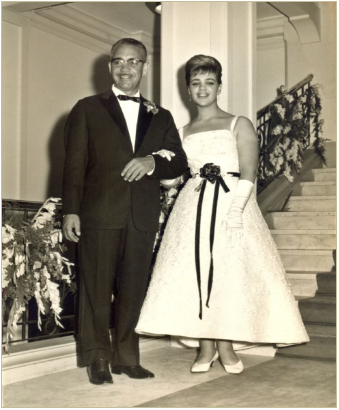
\includegraphics[width=0.7\linewidth]{13/debutando.png}
\caption{Debutando no Araraquarense.}
\end{figure}

Nem tudo eram flores, porém.
As festinhas de colégio continuavam a ser uma provação que me exigia elevada dose de estoicismo e teatral indiferença frente às minhas coleguinhas que exibiam seus corpinhos de ninfas em acrobáticos passos de \textit{rock n' roll} e \textit{hully-gully}.
Claro que a nenhum garoto ocorria convidar-me para uma empreitada dessa natureza.
Daí que, vagando ao largo das pistas de dança, acabei descobrindo pelos cantos, entre as vítimas do chamado ``chá-de-cadeira'', gente surpreendentemente interessante.
Um dia, essa descoberta se transformaria na certeza de que numa cidade tradicional e conservadora como a minha, é exatamente à margem que você vai encontrar as melhores figuras.
Também devo a essa fase outro importante aprendizado: meninos eram capazes de engrenar boas conversas quando, fora de um contexto de sedução, permitiam-se expor à vontade seus medos e inseguranças.
E, principalmente, suas opiniões e visões sobre o comportamento das garotas.
Essa iniciação no universo masculino foi especialmente útil no sentido de reforçar minha decisão de rejeitar firmemente o modelo feminino em voga, além de me despertar para o fato de que os rapazes eram, de longe, interlocutores bem mais estimulantes do que as moças.


Aos dezessete anos, terminado o Colegial, consegui meu primeiro grande triunfo: meus pais aceitaram que eu fizesse faculdade na Capital.
Confiando nos elogios que as minhas redações escolares sempre mereceram e acreditando nos efeitos do trabalho em que vinha me aplicando, ou seja, a construção da minha persona, escolhi fazer Jornalismo.
Mas a vitória tinha um preço: minha mãe queria me ver estudando no Sedes Sapientiae, faculdade agregada à Pontifícia Universidade Católica de São Paulo, conhecida por abrigar algumas dezenas de herdeiras das mais antigas famílias da sociedade paulistana.
Tal sonho começara a ser alimentado muitos anos antes, quando um extravagante italiano mudou-se para a minha cidade e, após construir um casarão de estilo florentino uma esquina abaixo da minha casa, lá acomodou-se com a mulher e uma filha que só aparecia nas férias.
Quando essa filha linda, suave e elegante, numa das suas habituais passagens por sob a nossa janela, contou a Dona Lectícia que cursava a Sedes Sapientiae, não houve mais quem tirasse da cabeça da mamãe que aquelas adoráveis maneiras se deviam à educação ministrada pelas Cônegas Agostinianas, dirigentes e proprietárias do tal estabelecimento.
Portanto, eu poderia fazer Jornalismo, se quisesse, mas teria que ser como opção secundária.
Porque do Sedes Sapientiae ela não arredava pé.
Concordei em candidatar-me lá ao curso de História.
Afinal, imaginei, cultura geral não seria demais para uma futura jornalista.

Ainda uma vez fui levada a um endocrinologista, o último e o mais sensato e ele me garantiu que, longe das pressões familiares, a embriaguez da liberdade certamente superaria os encantos da comida.
Preparei-me para deixar o casulo.
Poucos meses antes de embarcar, comecei a emagrecer.
Até arrumei um namorado.
Lindo.
Mas com uma voz ridícula, em falsete.
Livrei-me dele sem piedade.
Tinha coisas mais importantes em que pensar.

\chapter{}
Manina, ou Tia Maria Angelina, dezesseis anos mais velha que eu, foi como já disse, erigida em estrela-guia da minha penosa viagem através da adolescência.
A bem da verdade, sem jamais ter postulado tal distinção, pois, por toda a minha infância, muito mais frequentemente eu recebia atenção das amigas dela, sobretudo da meiga Lygia, do que dela própria.
Quando lhe falei, muitos anos depois, sobre o importante papel que desempenhara em minha vida, reagiu com divertido assombro.
Com certeza, em razão do fato de que, assumidamente e sob mais de um aspecto, ela jamais superou a própria adolescência.
Um Peter Pan de saias foi o que ela representou para mim.

Ao mudar-se com Vovô e Vovó para uma São Paulo infinitamente menor, com ares elegantes de metrópole europeia, titia começou a realizar suas aspirações de uma vida glamourosa e cosmopolita, batizada com algumas pitadas de discreta ousadia, impossível de ser vivida na acanhada Araraquara.
Manina se pretendia um tanto boêmia, amante da boa música que se ouvia pelos barzinhos da moda, dos bons filmes, dos espetáculos teatrais, sempre que possível desfrutados na companhia de homens de classe, atraentes e muito bem vestidos, atributos que, conquanto raros, só os autorizava a candidatar-se a uma relação pouco mais que platônica, como rapidamente descobriam.
Qualquer tentativa de avançar além disso, empacava diante de um bem amarrado nó górdio: o casamento não era uma opção válida para ela e outra alternativa seria inadmissível enquanto os pais vivessem.
Ela jamais daria aos pobres velhinhos esse desgosto.
Estabelecido o impasse, o admirável era que, nesse ponto, ela conseguia sair da encrenca, na maioria das vezes, convertendo o pretendente em amigo.
Mas, é claro, só me inteirei dessas estranhas particularidades da vida amorosa da tia já mocinha, quando fui estudar em São Paulo e, aí sim, tornei-me companhia constante dela e sua confidente, até.
Para a adolescente interiorana que eu fora até esse momento, ela sempre parecera o mais acabado exemplo de feminilidade moderna, independente, irresistível.


Para melhorar o modesto salário de funcionária pública, Tia Maria Angelina dava aulas de violão.
Como suas irmãs, tinha uma bela voz e uma sensibilidade intuitiva para a boa música.
Um dia, uma das suas alunas de violão, casada com um tal Alfredo Borba, diretor artístico da gravadora Odeon, cujo elenco reunia alguns dos mais festejados ídolos musicais da época, quis apresentá-la ao marido.
Bem impressionado, o sujeito propôs a ela gravar um disco simples, de 78 rotações, uma bolacha de acetato na qual eram impressas apenas duas canções, uma de cada lado.
Manina foi às nuvens.
E ali deu início a uma carreira ainda inédita na família -- a de compositora e cantora de música popular brasileira.

\begin{figure}
\centering
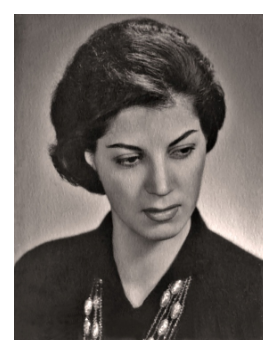
\includegraphics[width=0.7\linewidth]{14/manina-odeon.png}
\caption{Manina em foto artística para a gravadora Odeon.}
\end{figure}

Como acontecia com seus namoros, sua passagem pelo estrelato caracterizou-se pela fulguração meteórica.
Em poucos meses foi ao topo das paradas de sucesso, apresentou-se em boates famosas, em programas de rádio e televisão e, quando o sucesso começou a exigir as habituais contrapartidas em viagens, noitadas e contratos a serem cumpridos em vários lugares do país, Manina entrincheirou-se, mais uma vez, atrás de Vovó e Vovô.
Apresentando como desculpa o argumento de que já eram idosos e que ficavam apreensivos com as tentações do meio e de que ela não queria lhes causar preocupação, Deus-me-livre, etc., etc., ela voltou ao conforto seguro do anonimato.

Na carreira de funcionária pública, Manina comportou-se com diligência exemplar.
Talvez por isso não lhe faltou incentivo.
Ela chegou a ser chefe de seção na Secretaria da Fazenda e, anos depois, foi até transferida, a pedido, para a Casa Militar, no Palácio do Morumbi.
Os acréscimos de rendimento decorrentes dessas promoções e muita economia viabilizaram alguns outros sonhos que lhe eram caros: viajar para a Europa que, para ela, resumia-se praticamente à Itália, comprar um Fusquinha zero quilômetro e, mais tarde, adquirir um apartamento simples, mas bem situado, no Guarujá.

Houve uma vez em que o governo, oferecendo como estímulo a promessa de postos mais elevados e salários mais vantajosos, convidou seus funcionários a melhorar sua qualificação, facilitando-lhes o ingresso em cursos noturnos de faculdades públicas.
A maioria aderiu, entusiasmada.
Menos titia, que pretextou não poder voltar para casa tarde da noite, deixando Vovó, já então viúva, sozinha à espera.

Aos poucos, conhecendo Manina mais intimamente, comecei a me dar conta de estar na presença de uma personalidade, senão moderna e arrojada como eu julgara, pelo menos um bocado original, muito além do que supunha minha vã filosofia, para dizer o mínimo.

Uma vez um escritor, não lembro qual, declarou-se integrante da restrita parcela da humanidade capaz de ser feliz pela simples razão de ter a noção do que lhe é suficiente.
Pois, Tia Maria Angelina, estou certa, ocupou lugar de honra nessa confraria.
Foi um dos atributos que melhor a definiram e aquele que eu mais aprendi a admirar nela.
Sabia, com absoluta segurança, o que lhe convinha e não ambicionava um grama a mais.
Também não aceitava menos.
Em hipótese alguma.
Tudo quanto queria e fazia, tinha sua exata medida, não importando o que os outros dissessem.
Por isso, foi imune à inveja.
Alegrava-se genuinamente com o triunfo de parentes e amigos quando exibiam seus carrões, suas mansões ou falavam de viagens desfrutadas em \textit{resorts} deslumbrantes e restaurantes estrelados.
Porém, continuava a agradecer a Deus a felicidade proporcionada por suas próprias conquistas: o apartamentozinho do Guarujá, o seu adorado fusquinha e suas viagens econômicas para Roma.

Paradoxalmente, entretanto, gostava de ser vista como alguém familiarizado com luxo e sofisticação.
Era capaz de entrar no \textit{Copacabana Palace} e, fingindo displicência, pedir que lhe servissem um suco de laranja sob a pérgula.
Fez coisas assim muitas vezes e em variados lugares.
Sua aparência de manequim e elegância casual, na maioria das vezes, tornavam o teatrinho verossímil.
Essa mesma privilegiada aparência também lhe servia para navegar impávida em festas e \textit{vernissages}, desfilando trajes que ela se habituara a garimpar em liquidações e pontas de estoque, sem se sentir minimamente diminuída frente às joias e grifes carésimas exibidas pelas habituais frequentadoras desses ambientes.
Até gostava de alardear, com satisfação, quanto havia pago pela roupa, bolsa ou sapato, sempre que recebia elogios.


Entre suas contradições mais notórias, figurava um absoluto desinteresse por conhecer o Brasil, muito embora se declarasse patriota ardorosa, amante do samba, torcedora apaixonada do Corinthians e uma emocionada admiradora do Presidente Lula.
Contudo, sempre que chegava das suas viagens à Europa, nunca deixava de lamentar a feiura da nossa gente e das nossas cidades.
Até morrer, só abria exceção para o Rio de Janeiro.
Zona Sul, bem entendido.

Toda a independência e a quase ousadia que eu lhe atribuí ao longo da minha meninice, reduziram-se, quando a conheci melhor, à rebeldia de uma jovenzinha que, em presença do adulto, teimava em marcar posição.
Porque era engraçado como oscilava entre atitudes de aparente maturidade e objetividade frente aos problemas cotidianos e reações de insegurança e fragilidade muitas vezes infantis.
Aliás, muito embora fosse bastante alta para uma mulher da sua geração, media mais de um metro e setenta e cinco (nunca revelou quanto) e calçava número quarenta (particularidade também jamais admitida), para perplexidade das irmãs e sobrinhos, sempre teimou em comprar tudo pequeno para si: fusquinha, apartamentozinho, bicicletinha, panelinhas e sapatos invariavelmente um número menor.
E qualquer um que a presenteasse com roupas podia contar que ela haveria de sentar-se à máquina de costura para reformá-las ao seu jeito: vestidos seriam impiedosamente cortados até transformarem-se em casaquetos e mangas e golas reduzidas à metade.
Entre inconformada e zombeteira, minha mãe comentava que se alguém lhe desse um colete ela havia de dar um jeito de transformá-lo em boné! 

Enxergava-se emocionalmente como uma garotinha e quando as coisas ameaçavam ficar feias para o seu lado, refugiava-se num linguajar de criança, encolhendo-se e mostrando-se frágil demais para ser maltratada.

Contudo, encontrando brecha, nunca perdeu o gosto por desafiar.
Sempre adorou provocar os machos da família discutindo futebol ou política, assuntos que evidentemente estava bem longe de dominar.
O que não a impedia de defender seus estrábicos pontos de vista com veemência e por horas, até que só restasse aos sobrinhos e cunhados a alternativa de se dar por vencidos, para não ceder aos ímpetos de esganá-la.
Se houve uma coisa que nunca aceitou, foi ser alijada de uma discussão por ser mulher ou por não entender do assunto.


A despeito de ser totalmente egotista, duas grandes qualidades da Manina foram saber cultivar amizades e ter aversão à maledicência.
Tinha horror quase supersticioso de falar mal de quem quer que fosse.
Sua dedicação aos amigos nunca ultrapassava os limites da própria conveniência, mas era pródiga em pequenas atenções: telefonemas, lembrancinhas trazidas de viagens, convites eventuais para um cinema, uma peça de teatro, um almoço.
E mesmo quando esse ou aquele não lhe caía lá muito na simpatia, recorria ocasionalmente a uma espécie de compaixão genérica pela humanidade e convidava o infeliz para algum passeio.
Assim acontecia com a pobre Mariazinha, sua prima, uma implicante solteirona com quem se envolvia em calorosos arranca-rabos, mas que ela nunca deixou de chamar vez ou outra para sair, com pena do isolamento em que a deixavam irmãos, cunhadas e sobrinhos.

Tornava-se insuportável quando se deixava tomar de admiração por alguém, artista, político, jogador de futebol, não importa quem.
Beirava o fanatismo.
O sujeito imediatamente se revestia de todas as virtudes e que ninguém tentasse apontar no dito cujo um ou outro traço menos favorável de caráter que ela era bem capaz de avançar sobre o caluniador às unhadas.
 
Outra grande qualidade dela era saber ser grata.
Nunca esqueceu um favor recebido.
Nem desaforo, mas o sentimento causado por esse último, ela sabia disfarçar como ninguém.
Mesmo, por exemplo, quando a ofensa em questão recaia sobre o sofrido tempo vivido por João e Didi quando da falência da Mobiliadora, seu trauma maior.
Nada a feria mais fundo do que a suspeita de que houve algo de intencional no modo desastrado como Vovô conduziu o negócio.
Todavia, ainda assim, mesmo que lhe viessem lágrimas aos olhos quando ouvia insinuações de um Ópice ou outro, de que deviam ao Vovô a perda da fortuna paterna, engolia a dor.
Os primos sempre a ajudaram muito, justificava.
Mas, amargurava-se.
Porque Tia Maria Angelina idolatrava o pai, mais do que a mãe.
Morto Vovô, ela passou a vida a procurá-lo em todos os homens que conheceu.
Foi esse o segredo de polichinelo que desvendei, tão logo passei a conviver com ela.
Ela nunca quis um namorado, amante ou marido.
Ela queria um pai.
Mas tinha que ser aquele pai: o João, doce, amoroso, submisso.

A meu ver, entretanto, a coisa mais fantástica a respeito da Manina foi sua visão religiosa.
Daí lhe veio, sem dúvida, a tranquilidade e a confiança com que se permitiu fazer tudo o que bem entendeu nessa vida, sem embargo de ter sido, pela vida toda, não mais que uma reles funcionária pública, num país em que ser funcionária pública é o passaporte certo para uma vida de mediocridade sem esperança.
Manina parecia acreditar, com ingênua convicção, que tinha o Céu a seu serviço na maior parte do tempo.
Sentia-se especialmente protegida e abençoada e nem lhe passava pela cabeça perguntar-se quais eram suas credenciais para tão notória preferência.
Era assim e pronto.
A Virgem, os anjos e os santos, quando não o próprio Deus, em pessoa, livravam-na dos desastres, das doenças, dos assaltos e providenciavam o sol e o céu azul onde quer que ela chegasse.
E o pior é que, às vezes, a gente era quase obrigada a acreditar.
Pois, se houve um terremoto no país onde ela estava, Manina já ia longe, nem ficou sabendo.
Enchente, tornado, terrorismo? Só se foi depois que ela passou! Foi sempre econômica ao extremo e mesmo com seu mísero salário, após a morte da Vovó, manteve dois apartamentos, o carro, e ainda viajou várias vezes à Europa, aos Estados Unidos e à Argentina, graças às suas aplicações.
``-O meu macro'', como ela dizia, com ares de entendida.
Por influência do primo Rubens, um Ópice diretor de banco, a tia conseguiu taxas um pouco melhores para a aplicação das suas economias junto ao Banco Bradesco, nos tempos da inflação galopante dos anos 70.
Desde então, considerava-se uma privilegiada e, não importava quantos planos e sustos tivessem sacudido o país depois disso, ela nunca perdeu uma noite de sono sequer.
Tinha o seu ``macro...''

Passou por uma cirurgia séria no coração aos 68 anos e ao deixar a U.T.I, toda a queixa manifestada aos sobrinhos que, do lado de fora, esperavam por uma grave depressão pós-cirúrgica, foi a respeito do arroz ``muito empapado'' que lhe foi servido.
De resto, Deus foi bom, os médicos e enfermeiras muito atenciosos, quase não sentiu dor e ainda pôde acompanhar a novela todos os dias.

Em Cananéia, um dia, feliz porque acabara de comprar por uma ninharia uma blusa que vinha procurando há tempos, contou que entrou na igreja e, dirigindo-se ao Senhor, amorosamente censurou-o: 
{\itshape``-- Meu Deus, obrigada por ter-me feito encontrar assim tão baratinho a blusa que eu tanto queria.
Mas sabe, eu nem queria que o Senhor se preocupasse com uma coisa tão pequena! Às vezes o Senhor exagera!''}

Aos oitenta e dois anos, Tia Maria Angelina teve que refazer sua operação do coração.
A válvula instalada na cirurgia anterior esgarçou-se na aventura de uma excursão à Terra Santa, da qual havia chegado há apenas um mês.
Levei-a à emergência do hospital com pneumonia e um edema agudo de pulmão.
Um mês e uma semana depois, trouxe-a de volta para casa, de válvula nova, sã e salva.

Manina gostava de proclamar, orgulhosamente, ter poupado quantia suficiente para proporcionar a cada sobrinho, quando ela se fosse desse mundo, uma passagem de ida e volta à Europa.
E eu sempre retrucava, afirmando preferir barganhar a minha parte no tal espólio em troca da única coisa que realmente me interessava herdar dela: o seu Anjo da Guarda.

Aos noventa anos, Tia Manina já vira partir desse mundo, um a um, suas irmãs, seus amigos e experimentava a solidão e a amargura de viver sozinha em São Paulo, uma megalópolis impiedosa com os idosos.
A cada dez ou quinze dias, eu vinha de Cananéia para levá-la ao médico, fazer as compras da casa, dos remédios, atender, enfim às necessidades e problemas que a afligiam.
Não era suficiente.
Manifestando os primeiros sinais de demência senil a que se somou uma surdez irreversível, foi preciso encetar uma batalha dolorosa para derrubar o último e mais adorado bastião da sua autonomia: enviamos para Araraquara o seu fusquinha, o amado e sucateado Tatinho, que se tornara uma ameaça não só para ela própria  como para os vizinhos, transeuntes, bens e propriedades que se situassem no perímetro por onde ela circulava ao volante, olimpicamente  indiferente às buzinadas, xingamentos e expressões entre incrédulas e aterrorizadas dos circunstantes.
A essa seguiu-se outra luta, não menos cruel: acabamos por ter que enviar ela própria para Araraquara.
Paulinho, o sobrinho construtor, disponibilizara uma casa num dos seus condomínios, onde ela ficaria confortável e melhor assistida e, de lambuja, teria de volta, na garagem, completamente recuperado, o seu Tatinho!
Ainda assim, ela resistiu bravamente.
Num raro momento de lucidez, durante uma conversa na qual, pela enésima vez, eu argumentava que em Araraquara ela estaria melhor, mais segura, cercada dos sobrinhos e dos sobrinhos-netos, ela, pousando a mão sobre meu braço, interrompeu-me dizendo:
``-Teresa, eu não quis me casar, abri mão de ser mãe, de ter uma família.
Sempre soube que o preço seria terminar meus dias sozinha.''
Não obstante sua resistência, a deterioração acelerada das suas condições de saúde tornou a decisão de levá-la embora, inadiável.
Ainda viveu, como última alegria, o reencontro com seu fusquinha, novo como saído de fábrica e, mais que isso, pode dirigi-lo ainda algumas vezes nas ruas desertas do mais novo empreendimento do Paulinho, ainda em fase de implantação.
Faleceu à noite, sozinha como pressentira, numa clínica para idosos, para onde fora levada pouco tempo antes, quando já não havia como mantê-la longe de uma supervisão médica permanente.
Foi embora, deixando como lição maior para todos os que a conheceram, noventa e dois anos de uma existência que não perseguiu glória, nem fortuna, mas empenhou-se tão somente em fazer da Vida uma experiência que valeu a pena viver! 

\chapter{}
Cerca de seis meses depois de chegar a São Paulo, tranquei matrícula no curso de Jornalismo.
Como acontece com a maioria dos jovens, minhas fantasiosas expectativas sobre a profissão demonstraram ser totalmente equivocadas.
Como equivocada também estava minha auto-avaliação relativa à disposição para encarar a rotina de um ``foca'', naquela época.


A pioneira Faculdade de Jornalismo criada pelo jornal ``A Gazeta'' na qual eu fora admitida, era uma incipiente tentativa de dar a essa atividade um cunho mais profissional.
Até então, escrever para jornal era possível para políticos, advogados, literatos que juntassem prestígio ao domínio da língua ou, no caso do repórter, quando acaso, necessidade e oportunidade se juntavam para forjar um.
Jornalistas veteranos e bem conhecidos do público foram postos a nos dar aulas e pareciam perplexos e confusos diante da obrigação de nos transmitirem a ``técnica'' de escrever em jornal, algo sobre o que a maioria deles jamais teve tempo ou a iniciativa de pensar.
Escreviam e pronto.
{\itshape``-- Como é que se ensina vocação ou talento?''}, pareciam se perguntar.
Por esse motivo, as aulas resultavam, quase sempre, em longas digressões sobre as experiências de cada um, ou suas aventuras como correspondentes em lugares exóticos e situações extraordinárias.
Divertido, mas pouco produtivo.
Vendo que a coisa parecia não caminhar para lado algum, alguém da Direção deve ter concluído que o melhor era mesmo apelar para a boa e velha prática.
Assim, logo no princípio do segundo semestre, comunicaram-nos que teria início uma indispensável experiência para nossa adequada formação.
Um a um, fomos designados para um programa de estágio noturno nas delegacias de polícia da cidade de São Paulo, para colher notícias do palpitante submundo da Capital.
 Mesmo agraciada com a gentileza do meu orientador que, levando em conta minha pouca idade e minha condição feminina, destinou-me a uma delegacia mais ou menos central, à beira do Anhangabaú, o efeito sobre mim foi traumático.
Era demais para uma filha de Mathias Filpi, a vida inteira tão protegida do contato com o lado negro da realidade.
Nem cheguei a conhecer o tal antro.
Saí fora.
Decidi dedicar-me de corpo e alma ao meu curso na Sedes e, pior, para alegria da mamãe, substituí a Cásper Líbero pela mais burguesa das escolas, a EAD, ou seja, Escola de Artes e Decoração, uma escola alternativa para patricinhas desocupadas.
Diga-se, a meu favor, que não aguentei muito tempo aquele amontoado de pretensão e futilidade.
Mas, como qualquer saber acaba por ter alguma função, aprendi lá um pouco de História da Arte, pessimamente abordada na faculdade e desenvolvi certa habilidade para harmonizar móveis com tapetes e cortinas.
Mas, principalmente, convenci-me de que ninguém tem o direito de dizer a ninguém como deve morar.
E passei a execrar os decoradores.

O pensionato das Irmãs de São Vicente de Paula, congregação conhecida pelo alvo, engomado e medievalesco arranjo em forma de tricórnio que suas freiras usavam, ficava ao lado da Sedes Sapientiae, numa travessa da Rua Caio Prado.
A casa abrigava cerca de seis dezenas de universitárias, todas vindas do interior, como eu.
Preferi ficar num dos quartos individuais, na realidade celas da antiga clausura, pequenos e desconfortáveis, porém mais caros pelo luxo da privacidade, porque era bem do meu feitio me assegurar do terreno antes de sair fazendo novas relações.
Mas, meu isolamento não duraria muito.
Havia na casa um quarto com três camas, ocupado por apenas duas garotas inconformadas em dividir o ônus pela vaga vazia.
Uma delas, Ana Beatriz, sem nenhum constrangimento, tomou a peito a ingrata tarefa de conquistar minha simpatia e resolver o problema, fazendo de mim a terceira integrante do grupo.
Com seu sotaque limeirense e um sorriso invencível, postou-se à porta que eu mal entreabria à sua chegada, durante uma semana a fio, até convencer-me a acompanhá-la.
Fui apresentada então à sua colega de quarto, uma mineira neurótica, divertida e esguia como um galgo, estudante de Psicologia que à época, ou logo depois, não sei, namorou o Paulo, meu futuro marido.
Juntei-me a elas e aquele quarto, sabe-se lá por que, virou o ponto de encontro predileto da turma.
Todo mundo passava por ali quando voltava das aulas ou aos sábados, domingos e feriados.
Ali se sabia de tudo e de todos e eu reencontrei o prazer de conhecer e estudar a natureza humana.


Naquele tempo, ao chegarem a São Paulo, as ``mocinhas de família'' do interior, pois só mesmo espécimes dessa variedade de juventude feminina aceitariam se submeter às regras disciplinares tão rígidas quanto extemporâneas das Irmãs de São Vicente, experimentavam a um só tempo a emoção de se descobrirem relativamente livres da vigilância familiar e a de tomarem contato com a revolução cultural dos anos 60, cuja bandeira mais vistosa era a da liberação sexual proporcionada pelo advento da pílula.
Cinema Novo, Beatles, Bossa Nova, Existencialismo, Socialismo, Amor Livre, a juventude fervilhava em meio a uma catadupa de novas tendências e idéias, exacerbadas pela agitação política do período que haveria de desembocar no fechamento do regime e nos anos de chumbo da ditadura militar.
E tínhamos, para viver e digerir tudo isso, o tempo que ia das sete da manhã às nove da noite quando, impreterivelmente, nossas inefáveis hospedeiras cerravam as portas do pensionato e apagavam todas as luzes.
Aos sábados, é preciso reconhecer, as irmãs generosamente dilatavam o horário de recolhimento para as vinte e duas horas.
Quem tinha parentes em São Paulo escapava para a casa deles sempre que podia.
Por sorte, pouco tempo antes da minha chegada, Vó Didi, já então viúva, e Tia Maria Angelina tinham se mudado para seu novo apartamento, a duas quadras dali, na Rua Augusta.
Mas, sair do jugo das freiras para cair sob a guarda de avós, tios e primos não acrescentava grande coisa ao nosso projeto de libertação pessoal.
De modo que a participação de boa parte de nós, as mocinhas do pensionato, nos acontecimentos que marcaram a grande revolução dos costumes dos anos sessenta, ficou mesmo em nível de discussão, apenas.

Do mesmo modo, nossa contribuição política aos fatos que antecederam a chamada ``Redentora'', isto é, o golpe militar de 64, assim como aos movimentos de agitação e repressão que o sucederam, foi bastante contida pela vigilância dos parentes e pelos cuidados maternais das freiras, mas, neste caso, não aquelas do pensionato, mas das cônegas agostinianas, que as pobres Irmãs de S.Vicente não tinham alcance para entender o que se passava  além dos muros da clausura.
Já as cônegas agostinianas, uma exceção no universo feminino da Santa Madre Igreja, pois sua formação igualava-se às das mais cultas congregações masculinas, estas tomaram parte ativa nos acontecimentos da época, havendo até algumas delas, como Madre Cristina e Madre Mariângela, respectivamente a diretora do curso de Psicologia e a diretora da minha faculdade de História, que chegaram a merecer a atenção do DOPS, o sinistro aparelho policial da ditadura.
Éramos orientadas e incentivadas por elas a marchar nas passeatas de protesto que mobilizavam a classe estudantil ao longo daqueles anos, mas não deixava de ser ridícula a nossa preparação para tão arriscada empreitada: devíamos ir, sim, mas munidas do arsenal de segurança habitual, lencinhos molhados e ``carvãozinho'', um comprimido negro que trancava os intestinos blindando-os contra os efeitos das chamadas bombas de efeito moral e, o mais importante, vestidas em nossos \textit{tailleurzinhos} à Jackie Kennedy, meias de seda e salto alto (era assim que a maioria de nós frequentava as aulas).
Assim que a polícia atacasse, devíamos entrar nas lojas demonstrando convincente e extasiado interesse pelas vitrines, à feição de modernas Marias Antonietas, indiferentes ao tumulto que nos circundava.
E o engraçado era que funcionava mesmo.
Não era raro que os meganhas nos escoltassem para fora da confusão.

Aconteceu, entretanto, que pouco adiante do Sedes Sapientiae, situava-se a Rua Maria Antonia, campo de batalha onde se digladiavam os alunos do Mackenzie, direitistas fanáticos, acusados de acolher em suas hostes o famigerado CCC (Comando de Caça aos Comunistas) e os mais politizados estudantes da USP: aqueles da Escola de Sociologia e Política, da Faculdade de Economia e da Faculdade de Arquitetura e Urbanismo, ardorosos defensores das correntes de pensamento situadas à esquerda.
As escaramuças iniciais entre uns e outros evoluíram para batalhas verbais, em que palavras de ordem e acusações gritadas ao megafone cruzavam de um lado para outro da rua e chegaram à violência explícita num dia em que coquetéis molotov explodiram, provocando o incêndio do histórico prédio-sede da Universidade de São Paulo.
A repressão baixou com ferocidade e, a partir daí, o governo decidiu apressar a transferência da tradicional instituição pública para o então distante campus do Butantã.
Desalojados, os cabeças do movimento estudantil encontraram na insuspeitada Sedes Sapientiae, aos olhos dos militares uma inofensiva escola ``espera-marido'' conduzida por freirinhas meio subversivas, é verdade, mas, freirinhas, apesar de tudo, o lugar ideal para prosseguir com suas articulações, confiados na inibição que o hábito e a origem aristocrática das nossas monjas imporiam ao governador Abreu Sodré e seus sabujos fardados.
O estratagema funcionou durante algum tempo, o que nos possibilitou a todas um emocionante contato ao vivo e a cores com os lendários e desassombrados líderes do movimento estudantil: Wladimir Palmeira, Paeco, José Serra, José Dirceu (desde então já visto como bonitinho, mas nada confiável) e mais um monte de artistas e intelectuais engajados na luta contra a ditadura.
Lembro-me de um memorável show organizado de improviso no salão nobre da faculdade, a pedido de um hirsuto líder sindical anunciado pelo breve apelido de Lula e que, subindo ao palco, com voz rouca e língua presa, explicou-nos o motivo da iniciativa: arrecadar fundos em benefício dos operários em greve da Nitroquímica.
 Arrebanhadas às pressas pela cidade, uma a uma, foram chegando celebridades como Paulo Autran, Sérgio Ricardo e talentos ainda em cueiros como Chico Buarque, Toquinho e Taiguara.
Lembrança indelével me ficou de uma figura dramaticamente impressionante de menina esculpida em bronze, magra e séria, que cantou uma áspera canção, ``Carcará'', como se incorporasse o pequeno gavião da caatinga, prestes a voar sobre a platéia com seu nariz adunco, os dedos em garra, o olhar duro e brilhante de predador.
Maria Bethânia.


Por várias vezes, nossas salas de aula foram palco de assembleias- relâmpago exaltadas, inflamadas, prementes, da União Estadual dos Estudantes (U.E.E.) e da União Nacional dos Estudantes (U.N.E.).
Numa delas, vencendo a timidez, a inibição interiorana, desfeita numa gelatina trêmula, pedi a palavra e falei, nem me lembro o que, tomada pelo clima emocional, pela convicção imperante, absoluta e contagiosa de que nos cabia salvar o Brasil, e quiçá o mundo, da voracidade do imperialismo norte-americano.
A partir daí criei coragem, saí em campo, fui inscrita como segunda ou terceira secretária numa chapa da U.E.E concorrente a eleições adrede proibidas pelos militares, atirei-me com entusiasmo às passeatas, corri dos policiais na Rua Pinheiros e me refugiei numa padaria onde tive que ouvir desaforos de trabalhadores cansados e exasperados pelo transtorno que os impedia de voltar para casa, enquanto lá fora as bombas explodiam com estardalhaço.
E numa das mais assustadoras experiências deste período louco, vi-me trancada, um dia, com mais três centenas de estudantes no convento dos dominicanos, no célebre cerco que opôs a um bando de frades e àquele punhado de adolescentes, um contingente do II Exército armado até os dentes, capaz de fazer amarelar qualquer liderança do tráfico dos morros cariocas.
Após horas de laboriosas negociações entre Igreja e Estado que avançaram pela tarde e entraram pelo início da noite, nos permitiram sair, afinal, um a um, famintos e assustados, esgueirando-nos através de um corredor polonês de escudos e cassetetes, portando nossos livros e nossas únicas armas - guarda-chuvas, porque chovia até não poder mais naquele dia em São Paulo.

De outra vez, numa das últimas e mais reprimidas passeatas de estudantes, intelectuais e operários paulistas, marchávamos da Praça da República, enveredando pela Barão de Itapetininga em direção ao centro velho de São Paulo, quando os militares nos cercaram, ostentando o melhor do seu aparato bélico, em que se destacavam a cavalaria do exército, a polícia marítima e seus gigantescos porretes, cães, tanques, urutus e brucutus.
Orientados a isolar a cabeceira da multidão, onde supostamente estavam as lideranças do movimento subversivo, os soldados cortaram o desfile ao meio, o que nos permitiu a nós, que caminhávamos na retaguarda, buscar refúgio nos prédios próximos.
Com algumas amigas, pernas bambas de terror, fui parar, sei lá como, no décimo segundo andar de um daqueles edifícios, num minúsculo quarto-e-sala cujo morador, um senhor de idade, piedosamente nos abriu a porta.
 Escapamos por um triz.
Minha futura cunhada, colega de sala e de pensionato, Sila Maria, que estava mais à frente, teve que agachar-se no asfalto, tomou algumas bordoadas e foi metida num camburão.
Mesmo de \textit{tailleur} e salto alto.
Livrou-a da cana e de coisa muito pior, quem sabe, o parentesco com general estrelado.


Passado o perigo, já no início da noite, voltei para casa matutando sobre a conveniência de abandonar minha recém iniciada carreira de militante política.
Uma das regras fundamentais do meu código pessoal de conduta sempre foi a de não me meter \textbf{deliberadamente} em situações cujas consequências eu não pudesse enfrentar, por minha conta e risco.
E, definitivamente, olhando cara a cara a brutalidade e o despropósito da reação do governo aos que se opunham à ditadura recém instalada no país e, por outro lado, testemunhando atitudes emocionais e atabalhoadas de muitos amigos e conhecidos cujas vidas promissoras e mal despontadas os porões da repressão trituraram e devolveram em cacos, ou simplesmente ceifaram sem piedade, decidi que era hora de parar.
Havia pontos obscuros na história toda.
A ditadura era intolerável, isto era certo.
Mas, pelo quê mesmo íamos substituí-la?  Isto já não parecia tão claro.
Ou, pelo menos, algumas das propostas anunciadas sobre os palanques improvisados não me pareciam merecedoras dos riscos suicidas a que nos expúnhamos, fosse pela inexequibilidade face às circunstâncias, fosse pela radicalidade algo suspeita.


No ano seguinte terminei meu curso.
Tinha decidido militar, sim, por um mundo melhor, mas do modo como sabia e podia.
Exercendo minha profissão.
Indo além do mister de ensinar História.
Sendo educadora.
Mas, como tantas vezes comentei com meus alunos, provavelmente não teria chegado a desenvolver uma consciência política tão clara do meu papel na sociedade, se não tivesse feito parte dessa geração que viveu o que seria, por muitas décadas, o canto do cisne da militância política juvenil e idealista neste país.
 Ainda não surgiu outra.
Sem o fio condutor de um ideal, o fantástico potencial de realização dos jovens vem se perdendo em desordem pelo ambiente.
Desperdiçado no vandalismo e na violência gratuita das gangues, consumido pelas drogas, desviado para o consumismo obsessivo, para a rebeldia sem causa, para o culto tão exagerado quanto fútil ao próprio corpo.
É uma pena.
Queira Deus lhes seja restituído tão cedo quanto possível o direito de sonhar utopias, a ventura de repensar o mundo com a onipotência, a ousadia, a vitalidade e a paixão algo irresponsável que só na mocidade nos é permitido viver.


\chapter{}

\begin{figure}
\centering
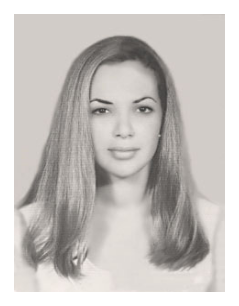
\includegraphics[width=0.7\linewidth]{16/carteira-de-trabalho.png}
\caption{Foto da minha primeira carteira de trabalho.}
\end{figure}

Aos vinte e um anos, obediente às recomendações da minha mãe, mesmo não sendo bonita eu \textbf{\textit{parecia}} sê-lo, após anos de aprendizado de como devia vestir-se, pentear-se, maquilar-se e comportar-se uma moça em sociedade.
Porque tal como predissera minha mãe, muito acertadamente, a convivência com as abonadas pupilas das cônegas agostinianas constituíra-se numa verdadeira escola de bom gosto e sofisticação.
Aprendizado reforçado pela assessoria da Tia Maria Angelina e das amigas de pensionato.
Os cabelos, agora longos, clareados e bem tratados, emolduravam um rosto mais harmônico, onde se destacava o nariz esculpido pelas hábeis mãos do Dr.
Fabrini, um renomado cirurgião plástico carioca.
Magra, ou pelo menos tão magra como jamais voltaria a ser, eu começava a achar divertida a situação de provocar admiração no público masculino.
Pela aferição das ruas, baseada em observações tão cruas quanto espontâneas de motoristas, pedreiros e \textit{office-boys}, eu me incluía entre as chamadas “boazudas”: alta, pernas grossas, quadris roliços e cintura fina.
A situação me era totalmente inusitada: provocar olhares à minha passagem, ser confundida com estrelinha de televisão, ver-me notada e seguida por rapazes, era uma novidade sem precedentes na minha vida.
Por sorte, paralelamente, havia trabalhado duro para superar minha timidez, melhorar minha capacidade de comunicação e conseguia com relativa facilidade impor-me frente à maioria das situações.
Em nenhum momento inebriei-me com essa admiração que eu, mais do que ninguém, sabia que resultava de pura ilusão ótica.
Não sou bonita, nunca fui, mas estava segura de produzir o efeito que uma vez um velho fazendeiro creditou à tia Odila: sem saber como definir o bem-estar que a sempre afirmativa presença dela lhe provocava, saiu-se com esta: “- Dona Odila, dá gosto ver a senhora assim, sempre tão \textbf{saudível e calorífera}!”.
É isso, tinha certeza de não ser bonita, mas desde a minha mocidade e até hoje, venho me empenhando em produzir a impressão de uma personalidade “saudível e calorífera”.
É o que pessoalmente designo como dever ecológico, isto é, a obrigação de contribuir para tornar o mundo um lugar mais agradável, exibindo uma aparência que tem menos a ver com elegância ou beleza e mais com certo jeito de ser.
No entanto, a descoberta de que podia exercer algum poder sobre o gênero superficial e tolo dos garanhões de plantão, tenho que admitir, encantou-me durante algum tempo e me manteve a salvo de interessar-me verdadeiramente por alguém.
Claro que para isso concorria também o fato de me conservar firme na disposição de jamais me casar.
Foi por essa altura que apareceu Paulo.

O ano que sucedeu à minha formatura, 1969, foi marcado pela derrubada de mais algumas fantasias que eu alimentava a meu próprio respeito.
Eu não queria voltar para Araraquara e procurava ansiosamente uma maneira de permanecer na Capital às minhas próprias custas.
Sabia que andava exigindo do meu pai mais do que era justo pretender.
Eu era a mais velha de cinco, já tinha passado da hora de saltar do berço.
Porém, sustentar-me com o salário de professora, em São Paulo só seria possível se eu tivesse coragem e iniciativa para aceitar trabalho onde aparecesse, o que podia significar tomar ônibus de manhã cedinho e voltar à noite, depois de enfrentar colégios públicos de periferia e renunciar às roupinhas, sapatinhos de moda e mais alguns adereços importantes para o meu recém-adquirido \textit{status} de beldade.
Na verdade, eu avançara muito pouco na direção da tão sonhada autonomia.
Na essência, continuava a mesma burguesinha assombrada por receios provincianos de enfrentar a selva da cidade grande e, mais do que isso, de viver por minha própria conta e risco, sem depender da mesada do papai.


Entrementes o governo, depois de longo tempo, decidiu promover em meados do ano um concurso para prover cargos de professores nas escolas públicas de todo o Estado de São Paulo.
Era a deixa que meu pai esperava para por fim à minha interminável, infrutífera e onerosa permanência em São Paulo.
Conformada, inscrevi-me, com a esperança de que até o concurso algum emprego aparecesse.
Estávamos em janeiro, ainda.

Um dia, andando pela faculdade, reencontrei Regina Pereira, minha antiga, esgalgada e neurótica companheira de quarto no pensionato.
Esfuziante, participou-me seu casamento no sábado seguinte e exigiu que eu me incluísse na comitiva de ex-colegas que se preparava para comparecer ao casório, em Poços de Caldas.
Fui.
No meio da festa, um rapaz sentou-se ao meu lado e não me largou mais.
Alto e magro, moreno como um árabe, olhos muito escuros, calado, não parecia nem um pouco divertido.
Ao contrário, era um tanto brusco e logo descobri que minhas táticas habituais de lidar com esse tipo de situação não funcionavam com ele.
Em pouco tempo desconstruiu todas e como costumava acontecer comigo quando me via desarmada e insegura, chorei.
Só então ele pareceu abrandar e decidiu ser gentil.
Comprou-me chocolates.
Ao voltar para São Paulo, estava decidida a esquecê-lo.
Ele me figurava uma ameaça.
Chamava-se Paulo e era um ex-namorado da noiva.
 
Dias depois, no Carnaval, fui para Araraquara porque participava de um bloco que desfilava no Clube todos os anos.
Estava eu lá, dançando na maior animação, quando uma amiga veio me avisar, um tanto preocupada, que um rapaz estava à minha espera no saguão.
A preocupação se justificava pelo fato de que minha família estava presente e meu pai, cujo gênio todos conheciam, já parecia sensivelmente alterado pelo uísque.
 Instintivamente, soube que era o Paulo.
Corri escada abaixo, disposta a despachá-lo para longe, evitando um previsível confronto.
Papai, desde alguns anos, vinha se convertendo num problema para todos nós.
Nunca soubemos se de alguma maneira pressentia a iminente doença cardíaca que o levaria ao túmulo, depois de limitar-lhe drasticamente a vida, ou se a aproximação da velhice e da decadência física lhe parecia intolerável porque mamãe, bem mais nova, estava no auge da sua disposição para a vida.
O fato é que papai vinha abusando sistematicamente da bebida e com isso se transformou numa versão particular de Dr.
JekiIl e Mr. Hyde: de dia, um homem equilibrado, sensato e bonachão; à noite, sob o efeito do álcool, um sujeito violento e imprevisível, capaz de atitudes de extrema agressividade e de completa falta de consideração por quem quer que fosse.
Como costuma acontecer nessas circunstâncias, evitávamos ao máximo levar amigos ou namorados em casa, eu mais do que os outros.
Mas, Paulo não era homem de se assustar com isso.
Eu ainda não sabia que, em matéria de loucura familiar, ele já conhecia tudo.
Não arredou pé e eu tremi sob os olhares arrevesados que meu pai lançava a intervalos sobre nós dois.
Consegui que Paulo concordasse em me levar para casa para afastá-lo dali, mas ainda nos despedíamos diante da porta quando o carro do meu pai virou a esquina acelerado, passou chispando por nós e invadiu a garagem sem reduzir a marcha.
Freou, guinchando, a centímetros da parede.
Gelada, ouvi, às minhas costas os argumentos desesperados da minha mãe, tentando fazer um alterado Mathias entrar sem dar vexame.
 Minha irmã, que chegara com eles no carro, através da janela entreaberta do nosso quarto, fazia sinais aflitos para eu entrar.
Finalmente, para meu alívio, Paulo decidiu ir embora.
Pulando a janela para não passar pela porta do quarto dos meus pais, onde a discussão prosseguia acalorada, estendi-me como um cadáver na cama, envolta na túnica, nas pulseiras e colares da minha fantasia tribal africana.
Acordei, na manhã seguinte, com minha mãe assustada pedindo que eu me levantasse e me arrumasse, porque “aquele moço” estava na varanda conversando com meu pai e, pelo que ela tinha entendido, os dois estavam saindo para ir ao clube tomar umas cervejas e conversar.
 Foi assim que Paulo entrou na minha vida para nunca mais sair.

\begin{figure}
\centering
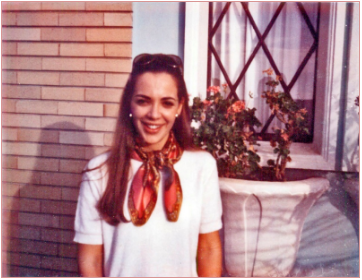
\includegraphics[width=0.7\linewidth]{16/eu-quando-paulo.png}
\caption{Eu, em 1969, quando conheci Paulo.}
\end{figure}

Ao longo das periódicas crises que o evoluir de um casamento propõe à gente, muitas vezes me perguntei se cheguei ao casamento por vontade própria ou se me deixei vencer pela tenacidade indomável do Paulo e pela capacidade extraordinária que ele tinha de reduzir a pó todo o meu tão bem arrumadinho sistema de defesa.
A verdade é que, com seu temperamento, ele expunha toda a frágil arquitetura da minha personalidade, tão cuidadosamente edificada ao longo dos anos para encobrir minhas inseguranças.
Eu levaria um longo tempo para entender que o que me punha em cheque era a exigência de verdade, de autenticidade que nele é permanente e intransigente.
Os traumas decorrentes da sua história familiar provocavam nele reações surpreendentes de intolerância a qualquer forma de manipulação ou jogo, por inocente que fosse.
Acostumei-me a compará-lo a um animal mal domesticado, cujo instinto alerta para a condição de ter no homem um inimigo natural e que, por uma folha que se agita, pode atirar-se sobre o dono, atacando-o.
Custei muito a aprender a lidar com esse jeito dele e a sensação constante de estar indefesa resultou na desconfiança de ter me tornado, eu sim, manipulável.

Hoje, passados muitos anos, inclino-me a concluir que ambos fomos envolvidos numa espécie de irresistível conspiração cósmica.
De outra maneira, como poderiam ter se juntado duas criaturas tão pouco propensas a acreditar em quem quer que fosse?

\chapter{}
Como filha mais velha de um casamento problemático, com fama de sensata e precocemente amadurecida, assumi, durante a adolescência, o papel de algodão entre cristais para amenizar o clima em casa.
Não por delegação de alguém, mas porque é sempre o que acaba naturalmente acontecendo.
Só que isto ficou muito pesado e, a partir de certo tempo, intuí que inútil, também.
Comecei a achar até que quanto mais depressa meus pais se vissem sozinhos, maior seria a possibilidade de eles recomporem sua relação.
Esse era um dos motivos de eu não querer voltar a morar em casa.
O outro, só vim a compreender com clareza muito mais tarde, e nada tinha a ver com a situação familiar, ao menos não diretamente – era a minha inconformidade com o medo que parece impregnar todo o modo araraquarense de ser: o medo de ser diferente e o medo de parecer igual; o medo de fracassar, mas também o de destacar-se pela vitória; o medo de tentar e o de deixar passar a oportunidade; o medo de tomar a frente que só se compara ao de ficar para trás; o medo, sempre o medo paralisante de tudo, que vai reduzindo as pessoas, secando-lhes a alma e a vontade, até transformá-las em zumbis.
Nem todas têm esse destino, é preciso admitir; apenas aquelas que se submetem ao imperativo ``de ser como todo mundo''.
As que se recusam a adequar-se, naquele ambiente de maledicência agressiva, têm que resignar-se a circular à margem ou migrar para outros ares.
É tema freqüente de conversa entre os que ficam, a enumeração de quantos araraquarenses tornaram-se pessoas reconhecidas depois que se mudaram da terra.
Mas, só depois que se mudaram da terra.

Quando conheci Paulo, duas coisas me despertaram imediata admiração: ele parecia não ter medo de nada e definitivamente se negava a ser ``como os outros''.
Seus caminhos nunca eram os convencionais e tudo o que causava receio nesta araraquarense para ele era ``bobagem''.
Parecia o antídoto perfeito para os males que me assombravam.
E, com outra característica absolutamente nova e surpreendente para mim que tinha crescido numa cultura de ``machões'': ele manifestava seu afeto com naturalidade e entrega, sem nenhum receio de parecer frágil.

Sempre que percorria a rodovia a caminho da capital, olhando pela janela do ônibus, eu me punha a imaginar para onde levariam aquelas estradinhas de terra que fugiam pelo meio das montanhas, buscando lugares quem sabe idílicos entre plantações e regatos, casas brancas e simples de cujas soleiras à noite se podia contar as estrelas como eu fazia na minha infância, e me vinha a desconfiança de que o sentido da Vida devia ser buscado lá, nos lugares para onde levavam essas estradinhas.
Algum tempo depois de conhecer Paulo, comecei a acreditar que se existia alguém nesse mundo em cuja companhia eu tentaria essa aventura, esse alguém era ele.


Prestei o concurso para professora, fui aprovada e quando chegou o momento da escolha, tinha à minha disposição as melhores vagas de Araraquara.
Só eu tinha logrado aprovação entre os candidatos da cidade.
No salão nobre da minha ex-escola, onde fui convocada a me apresentar para esta etapa do concurso, estavam presentes papai, mamãe e, firme ao meu lado, Paulo.
Havia uma vaga próxima a Piracicaba, onde ele fazia o último ano da faculdade de Agronomia, que ele havia pesquisado ``in loco'' e me pressionava a aceitar.
Desde os três meses de namoro, Paulo me cobrava casar com ele.
A idéia do casamento continuava a me parecer indigesta.
O exemplo de casa não me autorizava fazer bom juízo de tal instituição.
Mas, nos últimos tempos, a cobrança vinha se fazendo mais insistente e até exasperada.
 Agora eu estava presa numa armadilha: se escolhesse Araraquara, a reação do Paulo seria imprevisível; se escolhesse Piracicaba, seria duro flagrar a decepção dos meus pais.
Só consegui me resolver quando me conscientizei de que estava me decidindo, na verdade, pelo meu projeto de vida.
E meu projeto de vida passava longe de Araraquara.
Escolhi Piracicaba ou, melhor dizendo, Rio das Pedras, pouco mais que um vilarejo, próximo de lá.

Mais uma vez, meus pais me surpreenderam.
A mágoa foi inevitável, pude vê-la claramente na fisionomia dos dois.
Mas, de alguma maneira, parecem ter se dado conta de que a partir dali eu passava a trilhar meu próprio caminho.
E que nele eu andaria ao lado do Paulo, perceberam-no mesmo antes de mim.
Se alguma insegurança resultou disso, um receio de que eu me desse mal, nenhuma palavra me foi dita sobre isso.
Para todos os efeitos, eu tive a clara certeza de que acabara de ser emancipada.

\begin{figure}[H]
\hfill
\centering
\begin{subfigure}[h]{0.4\linewidth}
\centering
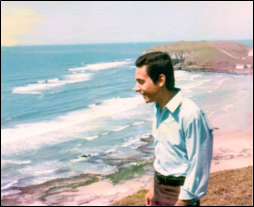
\includegraphics[width=\linewidth]{17/paulo-casamento.png}
\end{subfigure}
\hfill
\begin{subfigure}[h]{0.4\linewidth}
\centering
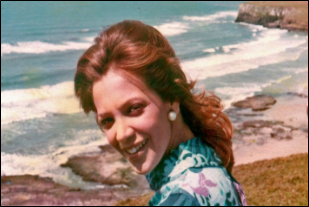
\includegraphics[width=1\linewidth]{17/teresa-casamento.png}
\end{subfigure}
\caption{Paulo e eu, aos vinte e seis anos, quando nos casamos.}
\end{figure}


\chapter{}

\begin{figure}
\centering
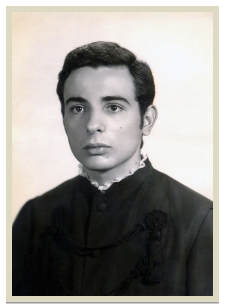
\includegraphics[width=0.8\linewidth]{17/paulo-formatura.png}
\caption{Paulo no dia da formatura.}
\end{figure}

Paulo formou-se em meados do ano de 1971 e foi trabalhar no Mato Grosso, na cidade de Campo Grande, num escritório de planejamento agrícola.
Marcamos nosso casamento para outubro daquele mesmo ano.
Transferi-me de volta para Araraquara, para ajudar minha mãe nas providências necessárias, uma vez que ela já estava envolvida com o casamento da minha irmã, marcado para apenas três meses antes do meu.


Não importa o que se diga a respeito do casamento, da sua sobrevivência enquanto instituição, a verdade inegável é que a cerimônia ainda é um momento de sonho na vida da maioria das mulheres.
Decidi que ia vivê-lo em toda sua plenitude e quis parecer bonita nesse dia como nunca antes.
Escolhi cuidadosamente cada item da festa, do vestido ao cardápio, passando pela música e pela decoração da pequena capela.
Paulo e eu queríamos uma cerimônia discreta, para poucas pessoas, para alívio dos meus pais.
O casamento da minha irmã assumiu proporções orientais, uma vez que ambas as famílias eram radicadas em Araraquara há muito tempo e por isso não houve como escapar de convidar meio mundo.

Ao anoitecer do dia dez de outubro de mil novecentos e setenta e um, ao entrar pelo braço do meu pai naquela capelinha e ouvir o murmúrio de admiração das pessoas ali reunidas, comecei a flutuar em direção ao altar.
Senti-me no centro de um palco iluminado.
Tudo o resto era figuração.
Inclusive o noivo, como confessei a ele mais tarde, depois da festa.


\begin{figure}[H]
\centering
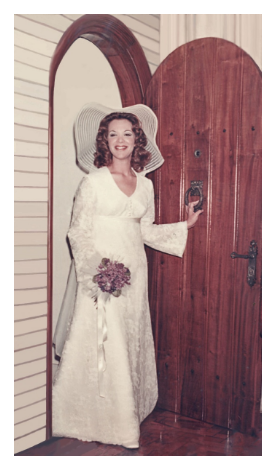
\includegraphics[width=0.5\linewidth]{17/vestida-casar.png}
\caption{Vestida para casar.}
\end{figure}

Em toda a minha história de vida naquela cidade, minhas aparições públicas tinham sido repetidamente um desastre.
Eu sempre fui o tipo de pessoa que escorrega no degrau, derruba a louça, esbarra nos móveis, pisa no pé do parceiro e esquece o discurso.
Na minha derradeira atuação, na formatura do curso colegial, tropecei no fio do microfone e, levando o dito cujo de cambulhada, ameacei varrer da mesa de honra todos os diplomas ali empilhados, na tentativa de me segurar, até que consegui finalmente me agarrar à mão de quem?  Dele mesmo, do meu algoz, o esquálido professor de Matemática que por pouco não rolou comigo num abraço solidário, palco abaixo.
A assistência foi ao delírio.
 

Mas, no dia do meu casamento, se, ao invés daquela minúscula nave, eu tivesse que palmilhar os tapetes de Westminster, eu o faria, com certeza, sem baixar o olhar uma única vez.
Ao longo da vida tenho recomendado às mocinhas que não dispensem a cerimônia de casamento.
Talvez não tenham outra oportunidade de se sentirem tão lindas como nesse dia.

\begin{figure}[H]
\centering
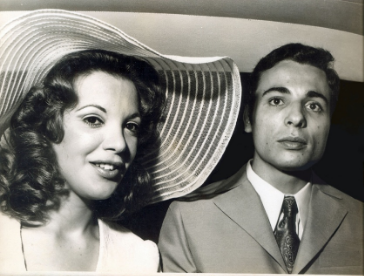
\includegraphics[width=0.75\linewidth]{17/no-carro.png}
\caption{No carro, já casados, a caminho da recepção.}
\end{figure}

Terminada a festa, partimos em lua de mel para o Rio Grande do Sul e, de lá, para Campo Grande, onde se desenrolaria a etapa inicial da nossa vida de casados.

Paulo tinha alugado um pequeno apartamento no centro, próximo ao escritório onde trabalhava.
Ganháramos um bocado de presentes e certa quantia em dinheiro da família dele, de modo que pude deixar tudo bem bonitinho, até com cortinas e todo o necessário para uma rotina doméstica confortável e aconchegante.
Descobri que tomar conta de casa me dava um insuspeitado prazer.
Gosto disso até hoje.
Só não contava com a inquietação do Paulo.

\chapter{}
Tenho a forte impressão de que a infância do meu marido transcorreu numa espécie de quarto escuro afetivo.
Seus pais se separaram quando ele era ainda muito pequeno para entender o que se passava.
Certa vez, almoçando com ele num pequeno restaurante da Rua Pinheiros, em São Paulo, fui surpreendida com uma das suas escassas memórias.
Lembrou que aquela era a casa onde sua família morou pouco antes da separação e, apontando para um canto do que tinha sido a sala, acrescentou: 
\textit{``-- Ali, depois de uma gritaria danada, vi minha mãe, do alto da escada, atirar sobre o meu pai um quadro, acho que até de um artista famoso.
O quadro afundou-lhe pescoço abaixo, deixando-o entalado na moldura, como naquelas comédias de pastelão.'' }

Quando perguntado sobre o que se passara antes ou depois do divórcio dos pais sempre se esquivou, dizendo que não havia muito que valesse a pena recordar.
Só contava que eles brigavam muito e que sua mãe vivia entrando e saindo de sucessivas internações em clínicas psiquiátricas, o que o deixava, na maior parte do tempo entregue a babás, empregadas e parentes.
Sua irmã referiu-se ao hábito dele de fugir de casa, desde pequeno.
Em outra de suas poucas lembranças, ele confirmou o que ela me disse, contando que um dia, ainda moleque, acompanhou um pipoqueiro conhecido nas suas andanças pela cidade o dia todo, só voltando para casa ao anoitecer.

Não gostava de comer.
Sua mãe dizia que vê-lo rolar o alimento na boca de uma bochecha para outra, interminavelmente, sem engolir, dava-lhe nos nervos e ela acabava entregando-o a uma paciente babá portuguesa.
Acabou anêmico e teve que ser levado ao médico porque tinha dificuldade de sustentar-se sobre as pernas.
Quando o conheci, se tivesse coisa mais interessante a fazer, era capaz de passar o dia inteiro com um sanduíche, esquecendo-se de se alimentar direito.

D. Yolanda, sua mãe, foi uma mulher bonita, elegante e inusitadamente culta para sua época.
Órfã de mãe muito cedo, sua vida foi sempre marcada pela convivência com tragédias.
Após a morte da mãe, de parto, ela e o irmão foram levados para viver a infância e a adolescência na casa dos tios, os Steidel, vitimados, também eles, pela trajetória de vergonha e sofrimento que culminou no suicídio do pai, Ernesto Steidel, injustamente acusado de desfalque na firma onde trabalhava.
A família e o episódio adquiriram notoriedade quando, instado pela mãe a provar a inocência do íntegro Ernesto, um dos filhos, Frederico Steidel, veio a se tornar um dos mais eminentes juristas desse país.
Nesse ambiente adulto, culturalmente elevado, mas obcecado pela ideia da restauração da honra familiar, as duas crianças, cujo pai constituiria uma nova família após passar uma longa temporada na Alemanha para aperfeiçoar seus estudos em Medicina Pediátrica, foram afetivamente compensadas com a satisfação indiscriminada de todas as vontades.
Sobretudo Yolanda, por natureza rebelde e geniosa.
À crônica de dramas familiares vivida pelos dois irmãos, um dia se somaria mais um.
O pai de ambos, o jovem e elegante Dr. José Augusto de Toledo Filho, que ao voltar da Europa abrira um consultório no centro da cidade, foi assassinado a tiros pelo marido enciumado de uma cliente.
Dessa história de vida, muito provavelmente, resultaram o espírito ágil e brilhante, mas também a neurose, a indisciplina e a infelicidade permanente da mãe de Paulo e sua tendência para a autodestruição.
E, como se não bastasse, tudo isso potencializado e agravado pelo casamento com José Ignácio, o pai do Paulo.

Conheci José Ignácio no auge da sua fama de intratável.
Foi antipatia à primeira vista.
Talvez até nem recíproca.
Porque, tenho que admitir, sempre recebi do meu sogro surpreendente e respeitosa consideração.
Que eu cautelosamente nunca pus à prova, mantendo até o fim, na presença dele, uma postura indevassável de índia do altiplano.
Ele era detentor de tal arrogância, de tão injustificada prepotência e de tão duvidoso senso de humor, que me espanta até hoje ele nunca ter sido moído a pauladas por um dos seus incontáveis desafetos.
Com o tempo, acabei até por entender um pouco a natureza estranha da desagradável criatura porque, ao final da sua vida, pude conhecê-lo melhor.
Quando adoeceu para morrer, coube ao Paulo cuidar dele e, dispondo-me a ajudá-lo nisso, descobri que José Ignácio era antes de tudo um medroso de marca maior.
Ele era afetado pelo maior de todos os medos, um medo doentio e absoluto de viver.
Não confiava em nada e em ninguém.
Muito menos em si mesmo, pois, por baixo de todos aqueles rompantes de poder, escondia um sentimento infantil de insuficiência.
Parecia ter necessidade de afirmar-se a todo instante para acreditar que existia.
Jamais se expressava com naturalidade; decretava, dissertava, perorava, parecendo encantar-se com o som da própria voz e com a extensão dos seus conhecimentos.
Sempre desconfiei de ciência que não se incorpora ao modo de ser do seu portador, capacitando-o a lidar melhor com a vida.
Pois José Ignácio era um típico caso desses.
Tinha uma memória prodigiosa capaz de acumular uma montanha de informações que ele, fluente em inglês e muito viajado, trazia dos quatro cantos do mundo, ou mandava buscar através de livros, revistas e publicações diversas.
Depois de memorizá-las, adorava despejá-las sobre o próximo, num monólogo delirante que deixava ao interlocutor apenas a tediosa função de emprestar-lhe os ouvidos e aplaudir no fim.
Um chato, em suma.
Mas essa capacidade de acumular e repetir o que lia, numa época em que memória e capacidade de aprender eram confundidas, erigiu-o em prodígio de inteligência para a família e, principalmente para os filhos, o que deu origem a previsíveis problemas para estes.
Eles nunca tiveram um pai, afetivamente falando, mas tinham um mito a respeitar, reverenciar e emular.

Uma outra característica do meu sogro marcou negativamente seus filhos.
Como ele, ao que parece, jamais conseguiu desenvolver uma personalidade adulta consistente, seus negócios nunca chegavam a bom termo.
Da sua busca insaciável por informações, sempre trazia engatilhadas ideias ainda não pensadas cá na província para grandes e inéditos investimentos destinados a produzir lucros fantásticos, o que lhe granjeou a fama adicional de homem de visão.
Ganhar muito dinheiro era outra das suas obsessões, compreensível para um sobrevivente da derrocada das elites cafeeiras.
Era o que eu chamava ``psicose da redenção''.
O problema, contudo, era que ele não conseguia tornar operativas tais ideias.
Montava o negócio, prosperava, enriquecia e então, em algum momento, tudo desmoronava, fosse pela sua incapacidade infantil de planejar e executar um empreendimento em bases reais, fosse pela dificuldade insuperável de relacionar-se com as pessoas.
Disso resultou que a vida de Paulo, seus irmãos e sua mãe foi sempre financeiramente imprevisível, instabilidade tornada ainda mais crítica pelos vários casamentos do pai e pela guerra instalada entre ele e Yolanda.


Paulo é, sem dúvida, entre os filhos, o mais parecido com a mãe.
Não só fisicamente, mas também no caráter indomável e afeito à liberdade.
Se isso o tornou claramente o predileto dela, por outro lado, acarretou-lhe a hostilidade permanente do pai.
A separação litigiosa de Yolanda e José Ignácio foi daquelas em que os filhos são usados como dardos atirados alternadamente contra um ou o outro contendor.
Inúmeras vezes, nas fases de aperto financeiro que atravessamos, atendi telefonemas de José Ignácio nos quais, ao mesmo tempo em que anunciava o envio de alguma ajuda, atribuía ao filho toda sorte de defeitos herdados da mãe que, no entender dele, condenavam Paulo ao eterno fracasso.
Isso só piorava o conceito já muito ruim que eu tinha do meu sogro.
No entanto, mesmo detestando-o, chamava-me a atenção aquela espécie de intuição que o levava, após longos meses de ausência, a ressurgir nesses momentos.
Parecia que de longe, permanentemente, ele monitorava a vida desse filho que teimava em fugir ao seu controle.
Porque Paulo, no final da adolescência, cansado daquela loucura familiar sem remédio e sem fim, um belo dia, no dizer de Yolanda, ``enrolou seu colchãozinho e se foi de casa para nunca mais voltar''.
Amparou-o um meio-irmão da mãe, Roberto, que vivia da atividade de comprar bois para grandes frigoríficos.


Esse tio era um indivíduo grande, machista, falastrão e engraçado, uma figura típica de uma fase legendária da pecuária brasileira, a das comitivas e do desbravamento do centro-oeste.
Ficou rico nessa atividade, sobrevoando no seu avião as fazendas de criação de gado das então remotas regiões do Pantanal mato-grossense e adjacências, organizando comitivas que de caminhão ou a passo, pelas estradas boiadeiras, traziam as reses para serem abatidas em São Paulo.
Essa vida aventurosa e meio nômade que fascinava pelo contato com lugares e tipos extraordinários, com certeza vinha de encontro às mais caras aspirações do Paulo: fuga e libertação.
E o melhor, Roberto parecia confiar nele para muito além do que do que sua idade e pouca experiência autorizavam.
Coisa que o pai jamais fez.
Roberto ainda bancou por um bom tempo a sua faculdade, coisa que o pai também declarou que não faria no momento mesmo em que o filho foi comunicar-lhe a sua aprovação no vestibular para a Escola Superior de Agronomia Luís de Queiroz, em Piracicaba.
Roberto gostava de ensinar ao sobrinho: \textit{``-- Nunca se meta em negócios pequenos.
Negócios pequenos quebram.
Negócios grandes apenas trincam.''}

\begin{figure}
\centering
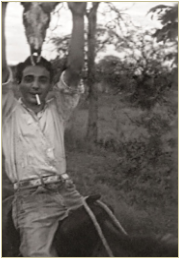
\includegraphics[width=0.6\linewidth]{19/no-pantanal.png}
\caption{Paulo no pantanal.}
\end{figure}

\begin{figure}
\centering
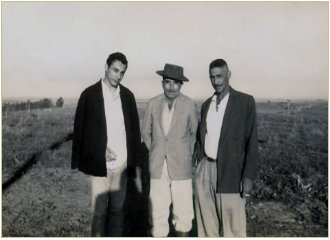
\includegraphics[width=0.85\linewidth]{19/comitiva.png}
\caption{Com os companheiros de comitiva.}
\end{figure}


\begin{figure}
\centering
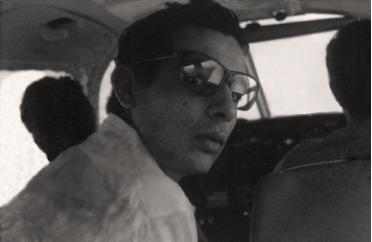
\includegraphics[width=0.85\linewidth]{19/voando+roberto.png}
\caption{Voando com Tio Roberto.}
\end{figure}

Não conheci outras pessoas cuja influência tenha sido decisiva na vida do Paulo.
Deve ter havido, mas não as conheci.
Mas, Yolanda, José Ignácio e Roberto conheci o suficiente para identificar de que maneira marcaram o seu jeito de ser.


Em comum, José Ignácio e Yolanda tinham a falta de limites e a dificuldade em orientar-se no mundo real.
Ela, por um ``panache'' que lhe era natural, não tinha medo de coisa alguma e não se curvava a nada.
A coragem nela era autêntica.
Mostrava ser, nos seus raros momentos de paz, uma grande entendedora da alma humana, lúcida e profunda, mas, nas fases de transtorno psíquico, seu humor e ironia, habitualmente tão sutis quanto divertidos, tornavam-se violentos e demolidores.
Então, não respeitava ninguém, fossem filhos, parentes, vizinhos, conhecidos, quem quer que se opusesse às suas vontades.


Era uma artista, fazia gravuras, delicadas pinturas e escrevia com graça e estilo.
Suas traduções do inglês, com as quais reforçava o orçamento após separar-se do marido, estão entre as melhores que já li.
Entretanto, tinha grande dificuldade em lidar com a realidade cotidiana e, principalmente, com as restrições que a vida de mãe de três filhos, separada de um marido psiquicamente desequilibrado e financeiramente instável, lhe impunham.
Tinha gostos sofisticados e, com alguma frequência torrava sua mesada quase instantaneamente com chás importados, bolos e queijos finos.
Além de montanhas de livros, claro.
Paulo conta que fazia coisas como receber a pensão do ex-marido, dinheiro que vez ou outra ela tinha de ir buscar na justiça, e contratar um táxi para levá-la ao litoral porque estava com vontade de velejar.
 

\begin{figure}
\centering
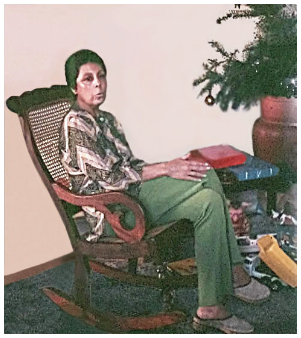
\includegraphics[width=0.8\linewidth]{19/d-yolanda.png}
\caption{D.Yolanda, por volta dos sessenta anos}
\end{figure}

Quando meus filhos eram pequenos e ela vinha visitar-nos, não conseguia conformar-se em ver-me enterrada naquela rotina de lecionar e cuidar dos meninos e da casa, entre fraldas e mamadeiras.
Dizia achar essa vida o cúmulo da mediocridade emburrecedora e andava atrás de mim, insistindo o tempo todo para que eu me sentasse para conversar sobre leituras e filmes.


Na sua própria casa, quando deixou José Ignácio e atravessou muitas fases de quase penúria, minha cunhada Marina conta, imitando-lhe o gesto refinado de sentar-se e acender um cigarro, que ela perguntava aos filhos, com cômica casualidade: - ``O que vocês acham de a gente abrir um bistrô?'' Sem levar em conta nem a falta de capital para tanto e nem o fato de que embora fizesse com certo domínio alguns pratos, cozinhava quando lhe dava na telha e sem muito critério.
Por exemplo, gostava de fazer um cozido português e o fazia bem.
Só que, quando isso acontecia, as crianças tinham que se preparar para comer o tal cozido a semana inteira, pois era só o que teriam até que ele acabasse.
Em José Inácio, a falta de limites e a valentia não me pareciam tão naturais e eu chego a acreditar que, embora lendárias, suas exibições em ambas as modalidades eram bastante seletivas -- só aconteciam quando ele se sentia seguro de que as circunstâncias, a surpresa ou a fraqueza do outro tornavam o revide improvável.
No fundo, constituíam-se apenas num \textit{mis-em-scène} destinado a obter para ele o reconhecimento de que carecia, orientado por um discutível senso de humor.
Porque a verdade é que José Ignácio era formalista ao extremo, reverenciava o poder e era grande apreciador das convenções sociais.
Gostava de vestir-se bem, era socialmente cavalheiresco no trato com as damas e revelava enorme apreço pelas tradições.
Era um cultor entusiasmado da genealogia paulista e suas origens familiares fincadas no bandeirantismo eram alardeadas \textit{ad nauseam}.
A desintegração da fortuna familiar que o atingiu na adolescência marcou-lhe fortemente a personalidade, com a adicional contribuição de uma mãe ``carola, ressentida e pouco iluminada'', conforme descrição da nora Yolanda.
Esta senhora, segundo minha sogra, descendente de tradicional família paulistana, enfrentou a perda do patrimônio na crise do café fazendo doces, quitandas e embutidos, com a ajuda das parentes, que mandava vender nas vizinhanças.
E José Ignácio, molecote ainda, era o escolhido para entregar as encomendas nas casas dos antigos colegas de brincadeiras e de escola.
Essa história de ter entregado, de porta em porta, as linguiças que a mãe fazia era recorrente nas suas reminiscências e parece ter contribuído para o sentimento de inadequação que dificultava sua relação com as pessoas.
Não que esse fosse um fato extraordinário numa época como aquela, de derrocada generalizada da aristocracia cafeeira.
O que, segundo minha sogra, marcou esse período a fogo na memória de José Ignácio foi a revolta sempre presente na fala, nos gestos e na expressão da mãe, D. Noêmia, inconformada por ver-se reduzida àquela condição.
É de se supor, também, que muita reza, muito conversa de culpa e castigo tenham sido ouvidas sob o teto daquela casa.
Porque Noêmia, sempre segundo Yolanda, responsabilizava o marido pela situação toda e atribuía a uma condenação divina as agruras que atormentavam a família.
Dois fatos testemunhados por mim, dão razão à minha sogra: o primeiro diz respeito à imensa quantidade de livros de oração antigos e muito manuseados pelas mulheres da família que eu vi na casa da irmã mais velha dele, Maria, logo após o falecimento dela e que eram representativos de uma rígida visão doutrinária, contemporânea da Contra Reforma ibérica; o outro, a menção constante que meu sogro fazia, nos seus últimos dias de vida, a punições e ao fogo do inferno e que surpreendia, numa pessoa informada como ele era, pelo que traduzia de uma visão física, concreta, da danação eterna instalada no seu inconsciente.
A relação culpa-castigo era muito firmemente plantada no ideário de José Ignácio.
Muito antes que as sucessivas isquemias fossem lhe restringindo a fala e os movimentos, a cada vez que morriam conhecidos ou parentes, ele costumava arrematar sua habitualmente cáustica análise da biografia do falecido, sentenciando: 
\textit{``-- Aqui se faz, aqui se paga!''}.

\begin{figure}
\centering
\includegraphics[width=0.8\linewidth]{19/yolanda+josé.png}
\caption{Yolanda e José Ignácio, recém-casados, passeando no Viaduto do Chá.}
\end{figure}

Arrisco-me a conjeturar que esta mentalidade seja a explicação plausível para o estoico silêncio com que suportou sua agonia final.
Ninguém conseguiu arrancar dele uma única queixa ou expressão de revolta.
Apenas ouvíamos o nome do filho, Paulo, chamado a toda hora como que para assegurar-se de tê-lo por perto, e curtos, e intensos gritos intermitentes que ele negava serem de dor.

\begin{figure}
\centering
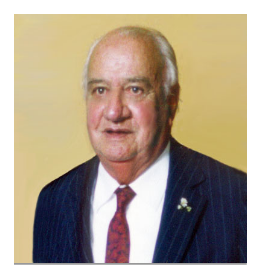
\includegraphics[width=0.8\linewidth]{19/josé.png}
\caption{José Ignácio, aos oitenta anos.}
\end{figure}

Ainda hoje, quarenta e um anos passados do dia em que conheci Paulo, posso dizer que ele esconde muitos enigmas que ninguém ainda desvendou.
Acredito que nem ele.
Porque Paulo parece não gostar de olhar para dentro de si mesmo e nem gosta de ser examinado de perto.
Sua permanente ansiedade trai medo e insegurança constantes cuja origem é fácil adivinhar, quando se conhece um pouco da sua história.
No entanto, disso mesmo provém sua grandeza.
Desconheço alguém que ao longo da vida tenha demonstrado tamanha coragem e persistência em enfrentar a própria fragilidade.
E, para mim, essa é a única medida que conta quando se avalia um ser humano.
Considerar a partir de onde e em que condições lançou-se na vida e verificar até onde conseguiu chegar.
Paulo, à meu ver, foi jogado no mundo sem a única defesa eficiente com a qual um indivíduo precisa contar -- a de ser reconhecido na infância, que permite a alguém saber quem de fato é.
Levando, além disso, na parca bagagem, instruções e mapas pouco confiáveis.
Aprendeu com a vida, literalmente.
Quase sozinho, por ensaio e erro.
E sobreviveu.
Foi longe, abriu caminhos, ousou, caiu e levantou.
Várias vezes.
Merece respeito.
Conseguiu ser o pai que ele nunca teve e, com sua experiência, pôde dar aos filhos o impulso necessário para que avancem até muito longe e com a serenidade e a confiança que ele próprio nunca experimentou.


\begin{figure}[H]
\centering
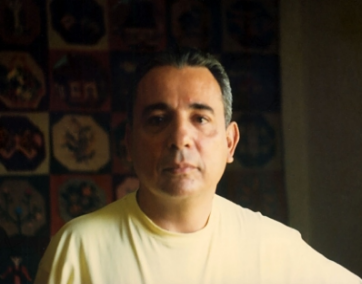
\includegraphics[width=0.9\linewidth]{19/paulo.png}
\caption{Paulo aos cinquenta anos.}
\end{figure}
\end{document}